%&preformat-disser
\RequirePackage[l2tabu,orthodox]{nag} % Раскомментировав, можно в логе получать рекомендации относительно правильного использования пакетов и предупреждения об устаревших и нерекомендуемых пакетах
% Формат А4, 14pt (ГОСТ Р 7.0.11-2011, 5.3.6)
\documentclass[a4paper,14pt,oneside,openany]{memoir}

%% Режим черновика
\makeatletter
\@ifundefined{c@draft}{
  \newcounter{draft}
  \setcounter{draft}{0}  % 0 --- чистовик (максимальное соблюдение ГОСТ)
                         % 1 --- черновик (отклонения от ГОСТ, но быстрая сборка итоговых PDF)
}{}
\makeatother

%% Использование в pdflatex шрифтов не по-умолчанию
\makeatletter
\@ifundefined{c@usealtfont}{
  \newcounter{usealtfont}
  \setcounter{usealtfont}{1}    % 0 --- шрифты на базе Computer Modern
                                % 1 --- использовать пакет pscyr, при его наличии
                                % 2 --- использовать пакет XCharter, при наличии подходящей версии
}{}
\makeatother

%%% Использование в xelatex и lualatex семейств шрифтов %%%
\makeatletter
\@ifundefined{c@fontfamily}{
  \newcounter{fontfamily}
  \setcounter{fontfamily}{1}  % 0 --- CMU семейство. Используется как fallback;
                              % 1 --- Шрифты от MS (Times New Roman и компания)
                              % 2 --- Семейство Liberation
}{}
\makeatother

%% Библиография

%% Внимание! При использовании bibtex8 необходимо удалить все
%% цитирования из  ../common/characteristic.tex
\makeatletter
\@ifundefined{c@bibliosel}{
  \newcounter{bibliosel}
  \setcounter{bibliosel}{1}           % 0 --- встроенная реализация с загрузкой файла через движок bibtex8; 1 --- реализация пакетом biblatex через движок biber
}{}
\makeatother

%%% Предкомпиляция tikz рисунков для ускорения работы %%%
\makeatletter
\@ifundefined{c@imgprecompile}{
  \newcounter{imgprecompile}
  \setcounter{imgprecompile}{0}   % 0 --- без предкомпиляции;
                                  % 1 --- пользоваться предварительно скомпилированными pdf вместо генерации заново из tikz
}{}
\makeatother
            % общие настройки шаблона
%%% Проверка используемого TeX-движка %%%
\RequirePackage{ifxetex, ifluatex}
\newif\ifxetexorluatex   % определяем новый условный оператор (http://tex.stackexchange.com/a/47579)
\ifxetex
    \xetexorluatextrue
\else
    \ifluatex
        \xetexorluatextrue
    \else
        \xetexorluatexfalse
    \fi
\fi

\newif\ifsynopsis           % Условие, проверяющее, что документ --- автореферат

\RequirePackage{etoolbox}[2015/08/02]               % Для продвинутой проверки разных условий
\providebool{presentation}

%%% Поля и разметка страницы %%%
\usepackage{pdflscape}                              % Для включения альбомных страниц
\usepackage{geometry}                               % Для последующего задания полей

%%% Математические пакеты %%%
\usepackage{amsthm,amsmath,amscd}   % Математические дополнения от AMS
\usepackage{amsfonts,amssymb}       % Математические дополнения от AMS
\usepackage{mathtools}              % Добавляет окружение multlined

%%%% Установки для размера шрифта 14 pt %%%%
%% Формирование переменных и констант для сравнения (один раз для всех подключаемых файлов)%%
%% должно располагаться до вызова пакета fontspec или polyglossia, потому что они сбивают его работу
\newlength{\curtextsize}
\newlength{\bigtextsize}
\setlength{\bigtextsize}{13.9pt}

\makeatletter
%\show\f@size                                       % неплохо для отслеживания, но вызывает стопорение процесса, если документ компилируется без команды  -interaction=nonstopmode
\setlength{\curtextsize}{\f@size pt}
\makeatother

%%% Кодировки и шрифты %%%
\ifxetexorluatex
    \usepackage{polyglossia}[2014/05/21]            % Поддержка многоязычности (fontspec подгружается автоматически)
\else
   %%% Решение проблемы копирования текста в буфер кракозябрами
    \ifnumequal{\value{usealtfont}}{0}{}{
        \input glyphtounicode.tex
        \input glyphtounicode-cmr.tex %from pdfx package
        \pdfgentounicode=1
    }
    \usepackage{cmap}                               % Улучшенный поиск русских слов в полученном pdf-файле
    \ifnumequal{\value{usealtfont}}{2}{}{
        \defaulthyphenchar=127                      % Если стоит до fontenc, то переносы не впишутся в выделяемый текст при копировании его в буфер обмена
    }
    \usepackage{textcomp}
    \usepackage[T1,T2A]{fontenc}                    % Поддержка русских букв
    \ifnumequal{\value{usealtfont}}{1}{% Используется pscyr, при наличии
        \IfFileExists{pscyr.sty}{\usepackage{pscyr}}{}  % Подключение pscyr
    }{}
    \usepackage[utf8]{inputenc}[2014/04/30]         % Кодировка utf8
    \usepackage[english, russian]{babel}[2014/03/24]% Языки: русский, английский
    \ifnumequal{\value{usealtfont}}{2}{
        % http://dxdy.ru/post1238763.html#p1238763
        \usepackage[scaled=0.960]{XCharter}[2017/12/19] % Подключение русифицированных шрифтов XCharter
        \usepackage[charter, vvarbb, scaled=1.048]{newtxmath}[2017/12/14]
        \setDisplayskipStretch{-0.078}
    }{}
\fi

%%% Оформление абзацев %%%
\usepackage{indentfirst}                            % Красная строка

%%% Цвета %%%
\ifpresentation
\else
    \usepackage[dvipsnames, table, hyperref]{xcolor} % Совместимо с tikz
\fi

%%% Таблицы %%%
\usepackage{longtable,ltcaption}                    % Длинные таблицы
\usepackage{multirow,makecell}                      % Улучшенное форматирование таблиц

%%% Общее форматирование
\usepackage{soulutf8}                               % Поддержка переносоустойчивых подчёркиваний и зачёркиваний
\usepackage{icomma}                                 % Запятая в десятичных дробях

%%% Оптимизация расстановки переносов и длины последней строки абзаца
\ifluatex
    \ifnumequal{\value{draft}}{1}{% Черновик
        \usepackage[hyphenation, lastparline, nosingleletter, homeoarchy,
        rivers, draft]{impnattypo}
    }{% Чистовик
        \usepackage[hyphenation, lastparline, nosingleletter]{impnattypo}
    }
\else
    \usepackage[hyphenation, lastparline]{impnattypo}
\fi

%%% Гиперссылки %%%
\usepackage{hyperref}[2012/11/06]

%%% Изображения %%%
\usepackage{graphicx}[2014/04/25]                   % Подключаем пакет работы с графикой

%%% Счётчики %%%
\usepackage[figure,table]{totalcount}               % Счётчик рисунков и таблиц
\usepackage{totcount}                               % Пакет создания счётчиков на основе последнего номера подсчитываемого элемента (может требовать дважды компилировать документ)
\usepackage{totpages}                               % Счётчик страниц, совместимый с hyperref (ссылается на номер последней страницы). Желательно ставить последним пакетом в преамбуле

%%% Продвинутое управление групповыми ссылками (пока только формулами) %%%
\ifpresentation
\else
    \ifxetexorluatex
        \usepackage{cleveref}                           % cleveref корректно считывает язык из настроек polyglossia
    \else
        \usepackage[russian]{cleveref}                  % cleveref имеет сложности со считыванием языка из babel. Такое решение русификации вывода выбрано вместо определения в documentclass из опасности что-то лишнее передать во все остальные пакеты, включая библиографию.
    \fi
    \creflabelformat{equation}{#2#1#3}                  % Формат по умолчанию ставил круглые скобки вокруг каждого номера ссылки, теперь просто номера ссылок без какого-либо дополнительного оформления
    \crefrangelabelformat{equation}{#3#1#4\cyrdash#5#2#6}   % Интервалы в русском языке принято делать через тире, если иное не оговорено
\fi

\ifnumequal{\value{draft}}{1}{% Черновик
    \usepackage[firstpage]{draftwatermark}
    \SetWatermarkText{DRAFT}
    \SetWatermarkFontSize{14pt}
    \SetWatermarkScale{15}
    \SetWatermarkAngle{45}
}{}

%%% Исправление положения якорей подписей (под)рисунков %%%
% Без hypcap и патча, при клике по ссылке на подрисунок, просмотрщик pdf прыгает "к подписи" а не "к рисунку".
% Подробнее: https://github.com/AndreyAkinshin/Russian-Phd-LaTeX-Dissertation-Template/issues/238
% (!) Даже с патчем, если мешать в одной фиге разные типы подфиг (subbottom и subcaption) - ссылки всё равно будут работать неправильно  (см. https://www.overleaf.com/read/czmbmmtnqrrg ).
\ifpresentation
\else
    \usepackage[all]{hypcap}

    \makeatletter
    \ltx@ifclasslater{memoir}{2018/12/13}{
        % Предполагается, что в следующей версии класс будет исправлен
        \typeout{Assuming this version of memoir is free from the jumping-to-caption bug.}
    }{
        \RequirePackage{xpatch}

        \newcommand\mem@step@subcounter{\refstepcounter{sub\@captype}\@contkeep}

        \xpatchcmd{\@memsubbody}%
        {\refstepcounter{sub\@captype}\@contkeep}% search pattern
        {}% replacement
        {\typeout{@memsubbody is patched}}%
        {\typeout{@memsubbody is NOT patched}}%

        \xpatchcmd{\@memcontsubbody}%
        {\refstepcounter{sub\@captype}\@contkeep}% pattern
        {}% replacement
        {\typeout{@memcontsubbody is patched}}%
        {\typeout{@memcontsubbody is NOT patched}}%

        \xpatchcmd{\@memsubfloat}%
        {\vbox\bgroup}% search pattern
        {\vbox\bgroup\mem@step@subcounter}% replacement
        {\typeout{@memsubfloat patch is ok}}%
        {\typeout{@memsubfloat patch is NOT ok}}%

        \xpatchcmd{\subcaption}%
        {\refstepcounter{sub\@captype}}% search pattern
        {\H@refstepcounter{sub\@captype}}% replacement
        {\typeout{subcaption second patch is ok}}%
        {\typeout{subcaption second patch is NOT ok}}%
    }
    \makeatother
\fi

%%% Цитата, не приводимая в автореферате:
% возможно, актуальна только для biblatex
%\newcommand{\citeinsynopsis}[1]{\ifsynopsis\else ~\cite{#1} \fi}
         % Пакеты общие для диссертации и автореферата
\synopsisfalse                      % Этот документ --- не автореферат
%%% Прикладные пакеты %%%
%\usepackage{calc}               % Пакет для расчётов параметров, например длины

%%% Для добавления Стр. над номерами страниц в оглавлении
%%% http://tex.stackexchange.com/a/306950
\usepackage{afterpage}

%%% Списки %%%
\usepackage{enumitem}

\usepackage{tikz}                   % Продвинутый пакет векторной графики
\usetikzlibrary{chains}             % Для примера tikz рисунка
\usetikzlibrary{shapes.geometric}   % Для примера tikz рисунка
\usetikzlibrary{shapes.symbols}     % Для примера tikz рисунка
\usetikzlibrary{arrows}             % Для примера tikz рисунка
\ifnumequal{\value{imgprecompile}}{1}{% Только если у нас включена предкомпиляция
    \usetikzlibrary{external}   % подключение возможности предкомпиляции
    \tikzexternalize[prefix=Dissertation/images/] % activate! % здесь можно указать отдельную папку для скомпилированных файлов
    \ifxetex
        \tikzset{external/up to date check={diff}}
    \fi
}{}
    % Пакеты для диссертации
\usepackage{tabu, tabulary}  %таблицы с автоматически подбирающейся шириной столбцов
\usepackage{fr-longtable}    %ради \endlasthead
\usepackage{rest-api}    %api
% sidewaysfigure
\usepackage{rotating}
% Листинги с исходным кодом программ
\usepackage{fancyvrb}
\usepackage{listings}
\lccode`\~=0\relax %Без этого хака из-за особенностей пакета listings перестают работать конструкции с \MakeLowercase и т. п. в (xe|lua)latex

% Русская традиция начертания греческих букв
\usepackage{upgreek} % прямые греческие ради русской традиции

%%% Микротипографика
%\ifnumequal{\value{draft}}{0}{% Только если у нас режим чистовика
%    \usepackage[final, babel, shrink=45]{microtype}[2016/05/14] % улучшает представление букв и слов в строках, может помочь при наличии отдельно висящих слов
%}{}

% Отметка о версии черновика на каждой странице
% Чтобы работало надо в своей локальной копии по инструкции
% https://www.ctan.org/pkg/gitinfo2 создать небходимые файлы в папке
% ./git/hooks
% If you’re familiar with tweaking git, you can probably work it out for
% yourself. If not, I suggest you follow these steps:
% 1. First, you need a git repository and working tree. For this example,
% let’s suppose that the root of the working tree is in ~/compsci
% 2. Copy the file post-xxx-sample.txt (which is in the same folder of
% your TEX distribution as this pdf) into the git hooks directory in your
% working copy. In our example case, you should end up with a file called
% ~/compsci/.git/hooks/post-checkout
% 3. If you’re using a unix-like system, don’t forget to make the file executable.
% Just how you do this is outside the scope of this manual, but one
% possible way is with commands such as this:
% chmod g+x post-checkout.
% 4. Test your setup with “git checkout master” (or another suitable branch
% name). This should generate copies of gitHeadInfo.gin in the directories
% you intended.
% 5. Now make two more copies of this file in the same directory (hooks),
% calling them post-commit and post-merge, and you’re done. As before,
% users of unix-like systems should ensure these files are marked as
% executable.
\ifnumequal{\value{draft}}{1}{% Черновик
   \IfFileExists{.git/gitHeadInfo.gin}{
      \usepackage[mark,pcount]{gitinfo2}
      \renewcommand{\gitMark}{rev.\gitAbbrevHash\quad\gitCommitterEmail\quad\gitAuthorIsoDate}
      \renewcommand{\gitMarkFormat}{\rmfamily\color{Gray}\small\bfseries}
   }{}
}{}

% Мои пакеты
\usepackage{blindtext}
\usepackage{pdfpages}
\usepackage{longtable}
\usepackage{float}
\usepackage{placeins}
   % Пакеты для специфических пользовательских задач

%%%%%%%%%%%%%%%%%%%%%%%%%%%%%%%%%%%%%%%%%%%%%%%%%%%%%%
%%%% Файл упрощённых настроек шаблона диссертации %%%%
%%%%%%%%%%%%%%%%%%%%%%%%%%%%%%%%%%%%%%%%%%%%%%%%%%%%%%

%%% Инициализирование переменных, не трогать!  %%%
\newcounter{intvl}
\newcounter{otstup}
\newcounter{contnumeq}
\newcounter{contnumfig}
\newcounter{contnumtab}
\newcounter{pgnum}
\newcounter{chapstyle}
\newcounter{headingdelim}
\newcounter{headingalign}
\newcounter{headingsize}
\newcounter{tabcap}
\newcounter{tablaba}
\newcounter{tabtita}
\newcounter{usefootcite}
%%%%%%%%%%%%%%%%%%%%%%%%%%%%%%%%%%%%%%%%%%%%%%%%%%

%%% Область упрощённого управления оформлением %%%

%% Интервал между заголовками и между заголовком и текстом
% Заголовки отделяют от текста сверху и снизу тремя интервалами (ГОСТ Р 7.0.11-2011, 5.3.5)
\setcounter{intvl}{1}               % Коэффициент кратности к размеру шрифта

%% Отступы у заголовков в тексте
\setcounter{otstup}{0}              % 0 --- без отступа; 1 --- абзацный отступ

%% Нумерация формул, таблиц и рисунков
\setcounter{contnumeq}{0}           % Нумерация формул: 0 --- пораздельно (во введении подряд, без номера раздела); 1 --- сквозная нумерация по всей диссертации
\setcounter{contnumfig}{0}          % Нумерация рисунков: 0 --- пораздельно (во введении подряд, без номера раздела); 1 --- сквозная нумерация по всей диссертации
\setcounter{contnumtab}{0}          % Нумерация таблиц: 0 --- пораздельно (во введении подряд, без номера раздела); 1 --- сквозная нумерация по всей диссертации

%% Оглавление
\setcounter{pgnum}{0}               % 0 --- номера страниц никак не обозначены; 1 --- Стр. над номерами страниц (дважды компилировать после изменения)
\settocdepth{subsubsection}            % до какого уровня подразделов выносить в оглавление
\setsecnumdepth{subsubsection}         % до какого уровня нумеровать подразделы


%% Текст и форматирование заголовков
\setcounter{chapstyle}{0}           % 0 --- разделы только под номером; 1 --- разделы с названием "Глава" перед номером
\setcounter{headingdelim}{1}        % 0 --- номер отделен пропуском в 1em или \quad; 1 --- номера разделов и приложений отделены точкой с пробелом, подразделы пропуском без точки; 2 --- номера разделов, подразделов и приложений отделены точкой с пробелом.

%% Выравнивание заголовков в тексте
\setcounter{headingalign}{1}        % 0 --- по центру; 1 --- по левому краю

%% Размеры заголовков в тексте
\setcounter{headingsize}{0}         % 0 --- по ГОСТ, все всегда 14 пт; 1 --- пропорционально изменяющийся размер в зависимости от базового шрифта


%% Подпись таблиц
\setcounter{tabcap}{0}              % 0 --- по ГОСТ, номер таблицы и название разделены тире, выровнены по левому краю, при необходимости на нескольких строках; 1 --- подпись таблицы не по ГОСТ, на двух и более строках, дальнейшие настройки: 
%Выравнивание первой строки, с подписью и номером
\setcounter{tablaba}{2}             % 0 --- по левому краю; 1 --- по центру; 2 --- по правому краю
%Выравнивание строк с самим названием таблицы
\setcounter{tabtita}{1}             % 0 --- по левому краю; 1 --- по центру; 2 --- по правому краю
%Разделитель записи «Таблица #» и названия таблицы
\newcommand{\tablabelsep}{ }

%% Подпись рисунков
%Разделитель записи «Рисунок #» и названия рисунка
\newcommand{\figlabelsep}{~\cyrdash\ } % (ГОСТ 2.105, 4.3.1) % "--- здесь не работает

%%% Цвета гиперссылок %%%
% Latex color definitions: http://latexcolor.com/
%\definecolor{linkcolor}{rgb}{0.9,0,0}
\definecolor{citecolor}{rgb}{0,0,0}
\definecolor{urlcolor}{rgb}{0,0,1}
\definecolor{linkcolor}{rgb}{0,0,0} %black
%\definecolor{citecolor}{rgb}{0,0,0} %black
%\definecolor{urlcolor}{rgb}{0,0,0} %black      % Упрощённые настройки шаблона

% Новые переменные, которые могут использоваться во всём проекте
% ГОСТ 7.0.11-2011
% 9.2 Оформление текста автореферата диссертации
% 9.2.1 Общая характеристика работы включает в себя следующие основные структурные
% элементы:
% актуальность темы исследования;
\newcommand{\actualityTXT}{Актуальность темы.}
% степень ее разработанности;
\newcommand{\progressTXT}{Степень разработанности темы.}
% цели и задачи;
\newcommand{\aimTXT}{Целью}
\newcommand{\tasksTXT}{задачи}
% научную новизну;
\newcommand{\noveltyTXT}{Научная новизна:}
% теоретическую и практическую значимость работы;
%\newcommand{\influenceTXT}{Теоретическая и практическая значимость}
% или чаще используют просто
\newcommand{\influenceTXT}{Практическая значимость}
% методологию и методы исследования;
\newcommand{\methodsTXT}{Методология и методы исследования.}
% положения, выносимые на защиту;
\newcommand{\defpositionsTXT}{Основные положения, выносимые на~защиту:}
% степень достоверности и апробацию результатов.
\newcommand{\reliabilityTXT}{Достоверность}
\newcommand{\probationTXT}{Апробация работы.}

\newcommand{\contributionTXT}{Личный вклад.}
\newcommand{\publicationsTXT}{Публикации.}


%%% Заголовки библиографии:

% для автореферата:
\newcommand{\bibtitleauthor}{Публикации автора по теме диссертации}

% для стиля библиографии `\insertbiblioauthorgrouped`
\newcommand{\bibtitleauthorvak}{В изданиях из списка ВАК РФ}
\newcommand{\bibtitleauthorscopus}{В изданиях, входящих в международную базу цитирования Scopus}
\newcommand{\bibtitleauthorwos}{В изданиях, входящих в международную базу цитирования Web of Science}
\newcommand{\bibtitleauthorother}{В прочих изданиях}
\newcommand{\bibtitleauthorconf}{В сборниках трудов конференций}

% для стиля библиографии `\insertbiblioauthorimportant`:
\newcommand{\bibtitleauthorimportant}{Наиболее значимые \protect\MakeLowercase\bibtitleauthor}

% для списка литературы в диссертации и списка чужих работ в автореферате:
\newcommand{\bibtitlefull}{Список использованных источников} % (ГОСТ Р 7.0.11-2011, 4)
         % Новые переменные, для всего проекта

%%% Основные сведения %%%
\newcommand{\thesisAuthorLastName}{\todo{Фамилия}}
\newcommand{\thesisAuthorOtherNames}{\todo{Имя Отчество}}
\newcommand{\thesisAuthorInitials}{\todo{И.\,О.}}
\newcommand{\thesisAuthor}             % Диссертация, ФИО автора
{%
    \texorpdfstring{% \texorpdfstring takes two arguments and uses the first for (La)TeX and the second for pdf
        \thesisAuthorLastName~\thesisAuthorOtherNames% так будет отображаться на титульном листе или в тексте, где будет использоваться переменная
    }{%
        \thesisAuthorLastName, \thesisAuthorOtherNames% эта запись для свойств pdf-файла. В таком виде, если pdf будет обработан программами для сбора библиографических сведений, будет правильно представлена фамилия.
    }
}
\newcommand{\thesisAuthorShort}        % Диссертация, ФИО автора инициалами
{\thesisAuthorInitials~\thesisAuthorLastName}
%\newcommand{\thesisUdk}                % Диссертация, УДК
%{\todo{xxx.xxx}}
\newcommand{\thesisTitle}              % Диссертация, название
{\todo{Длинное название диссертационной работы, состоящее из~достаточно большого
количества слов, совсем длинное длинное длинное длинное название, из~которого
простому обывателю знакомы, в~лучшем случае, лишь отдельные слова}}
\newcommand{\thesisSpecialtyNumber}    % Диссертация, специальность, номер
{\todo{XX.XX.XX}}
\newcommand{\thesisSpecialtyTitle}     % Диссертация, специальность, название (название взято с сайта ВАК для примера)
{\todo{Технология обработки, хранения и~переработки злаковых, бобовых культур,
крупяных продуктов, плодоовощной продукции и~виноградарства}}
%% \newcommand{\thesisSpecialtyTwoNumber} % Диссертация, вторая специальность, номер
%% {\todo{XX.XX.XX}}
%% \newcommand{\thesisSpecialtyTwoTitle}  % Диссертация, вторая специальность, название
%% {\todo{Теория и~методика физического воспитания, спортивной тренировки,
%% оздоровительной и~адаптивной физической культуры}}
\newcommand{\thesisDegree}             % Диссертация, ученая степень
{\todo{кандидата физико-математических наук}}
\newcommand{\thesisDegreeShort}        % Диссертация, ученая степень, краткая запись
{\todo{канд. физ.-мат. наук}}
\newcommand{\thesisCity}               % Диссертация, город написания диссертации
{\todo{Город}}
\newcommand{\thesisYear}               % Диссертация, год написания диссертации
{\todo{20XX}}
\newcommand{\thesisOrganization}       % Диссертация, организация
{\todo{Федеральное государственное автономное образовательное учреждение высшего
образования <<Длинное название образовательного учреждения <<АББРЕВИАТУРА>>}}
\newcommand{\thesisOrganizationShort}  % Диссертация, краткое название организации для доклада
{\todo{НазУчДисРаб}}

\newcommand{\thesisInOrganization}     % Диссертация, организация в предложном падеже: Работа выполнена в ...
{\todo{учреждении с~длинным длинным длинным длинным названием, в~котором
выполнялась данная диссертационная работа}}

%% \newcommand{\supervisorDead}{}           % Рисовать рамку вокруг фамилии
\newcommand{\supervisorFio}              % Научный руководитель, ФИО
{\todo{Фамилия Имя Отчество}}
\newcommand{\supervisorRegalia}          % Научный руководитель, регалии
{\todo{уч. степень, уч. звание}}
\newcommand{\supervisorFioShort}         % Научный руководитель, ФИО
{\todo{И.\,О.~Фамилия}}
\newcommand{\supervisorRegaliaShort}     % Научный руководитель, регалии
{\todo{уч.~ст.,~уч.~зв.}}

%% \newcommand{\supervisorTwoDead}{}        % Рисовать рамку вокруг фамилии
%% \newcommand{\supervisorTwoFio}           % Второй научный руководитель, ФИО
%% {\todo{Фамилия Имя Отчество}}
%% \newcommand{\supervisorTwoRegalia}       % Второй научный руководитель, регалии
%% {\todo{уч. степень, уч. звание}}
%% \newcommand{\supervisorTwoFioShort}      % Второй научный руководитель, ФИО
%% {\todo{И.\,О.~Фамилия}}
%% \newcommand{\supervisorTwoRegaliaShort}  % Второй научный руководитель, регалии
%% {\todo{уч.~ст.,~уч.~зв.}}

\newcommand{\opponentOneFio}           % Оппонент 1, ФИО
{\todo{Фамилия Имя Отчество}}
\newcommand{\opponentOneRegalia}       % Оппонент 1, регалии
{\todo{доктор физико-математических наук, профессор}}
\newcommand{\opponentOneJobPlace}      % Оппонент 1, место работы
{\todo{Не очень длинное название для места работы}}
\newcommand{\opponentOneJobPost}       % Оппонент 1, должность
{\todo{старший научный сотрудник}}

\newcommand{\opponentTwoFio}           % Оппонент 2, ФИО
{\todo{Фамилия Имя Отчество}}
\newcommand{\opponentTwoRegalia}       % Оппонент 2, регалии
{\todo{кандидат физико-математических наук}}
\newcommand{\opponentTwoJobPlace}      % Оппонент 2, место работы
{\todo{Основное место работы c длинным длинным длинным длинным названием}}
\newcommand{\opponentTwoJobPost}       % Оппонент 2, должность
{\todo{старший научный сотрудник}}

%% \newcommand{\opponentThreeFio}         % Оппонент 3, ФИО
%% {\todo{Фамилия Имя Отчество}}
%% \newcommand{\opponentThreeRegalia}     % Оппонент 3, регалии
%% {\todo{кандидат физико-математических наук}}
%% \newcommand{\opponentThreeJobPlace}    % Оппонент 3, место работы
%% {\todo{Основное место работы c длинным длинным длинным длинным названием}}
%% \newcommand{\opponentThreeJobPost}     % Оппонент 3, должность
%% {\todo{старший научный сотрудник}}

\newcommand{\leadingOrganizationTitle} % Ведущая организация, дополнительные строки. Удалить, чтобы не отображать в автореферате
{\todo{Федеральное государственное бюджетное образовательное учреждение высшего
профессионального образования с~длинным длинным длинным длинным названием}}

\newcommand{\defenseDate}              % Защита, дата
{\todo{DD mmmmmmmm YYYY~г.~в~XX часов}}
\newcommand{\defenseCouncilNumber}     % Защита, номер диссертационного совета
{\todo{Д\,123.456.78}}
\newcommand{\defenseCouncilTitle}      % Защита, учреждение диссертационного совета
{\todo{Название учреждения}}
\newcommand{\defenseCouncilAddress}    % Защита, адрес учреждение диссертационного совета
{\todo{Адрес}}
\newcommand{\defenseCouncilPhone}      % Телефон для справок
{\todo{+7~(0000)~00-00-00}}

\newcommand{\defenseSecretaryFio}      % Секретарь диссертационного совета, ФИО
{\todo{Фамилия Имя Отчество}}
\newcommand{\defenseSecretaryRegalia}  % Секретарь диссертационного совета, регалии
{\todo{д-р~физ.-мат. наук}}            % Для сокращений есть ГОСТы, например: ГОСТ Р 7.0.12-2011 + http://base.garant.ru/179724/#block_30000

\newcommand{\synopsisLibrary}          % Автореферат, название библиотеки
{\todo{Название библиотеки}}
\newcommand{\synopsisDate}             % Автореферат, дата рассылки
{\todo{DD mmmmmmmm YYYY года}}

% To avoid conflict with beamer class use \providecommand
\providecommand{\keywords}%            % Ключевые слова для метаданных PDF диссертации и автореферата
{}
             % Основные сведения
%%% Кодировки и шрифты %%%
\ifxetexorluatex
    \setmainlanguage[babelshorthands=true]{russian}    % Язык по-умолчанию русский с поддержкой приятных команд пакета babel
    \setotherlanguage{english}                         % Дополнительный язык = английский (в американской вариации по-умолчанию)

    % Проверка существования шрифтов. Недоступна в pdflatex
    \ifnumequal{\value{fontfamily}}{1}{
        \IfFontExistsTF{Times New Roman}{}{\setcounter{fontfamily}{0}}
    }{}
    \ifnumequal{\value{fontfamily}}{2}{
        \IfFontExistsTF{LiberationSerif}{}{\setcounter{fontfamily}{0}}
    }{}

    \ifnumequal{\value{fontfamily}}{0}{                    % Семейство шрифтов CMU. Используется как fallback
        \setmonofont{CMU Typewriter Text}                  % моноширинный шрифт
        \newfontfamily\cyrillicfonttt{CMU Typewriter Text} % моноширинный шрифт для кириллицы
        \defaultfontfeatures{Ligatures=TeX}                % стандартные лигатуры TeX, замены нескольких дефисов на тире и т. п. Настройки моноширинного шрифта должны идти до этой строки, чтобы при врезках кода программ в коде не применялись лигатуры и замены дефисов
        \setmainfont{CMU Serif}                            % Шрифт с засечками
        \newfontfamily\cyrillicfont{CMU Serif}             % Шрифт с засечками для кириллицы
        \setsansfont{CMU Sans Serif}                       % Шрифт без засечек
        \newfontfamily\cyrillicfontsf{CMU Sans Serif}      % Шрифт без засечек для кириллицы
    }

    \ifnumequal{\value{fontfamily}}{1}{                    % Семейство MS шрифтов
        \setmonofont{Courier New}                          % моноширинный шрифт
        \newfontfamily\cyrillicfonttt{Courier New}         % моноширинный шрифт для кириллицы
        \defaultfontfeatures{Ligatures=TeX}                % стандартные лигатуры TeX, замены нескольких дефисов на тире и т. п. Настройки моноширинного шрифта должны идти до этой строки, чтобы при врезках кода программ в коде не применялись лигатуры и замены дефисов
        \setmainfont{Times New Roman}                      % Шрифт с засечками
        \newfontfamily\cyrillicfont{Times New Roman}       % Шрифт с засечками для кириллицы
        \setsansfont{Arial}                                % Шрифт без засечек
        \newfontfamily\cyrillicfontsf{Arial}               % Шрифт без засечек для кириллицы
    }

    \ifnumequal{\value{fontfamily}}{2}{                    % Семейство шрифтов Liberation (https://pagure.io/liberation-fonts)
        \setmonofont{LiberationMono}[Scale=0.87] % моноширинный шрифт
        \newfontfamily\cyrillicfonttt{LiberationMono}[     % моноширинный шрифт для кириллицы
            Scale=0.87]
        \defaultfontfeatures{Ligatures=TeX}                % стандартные лигатуры TeX, замены нескольких дефисов на тире и т. п. Настройки моноширинного шрифта должны идти до этой строки, чтобы при врезках кода программ в коде не применялись лигатуры и замены дефисов
        \setmainfont{LiberationSerif}                      % Шрифт с засечками
        \newfontfamily\cyrillicfont{LiberationSerif}       % Шрифт с засечками для кириллицы
        \setsansfont{LiberationSans}                       % Шрифт без засечек
        \newfontfamily\cyrillicfontsf{LiberationSans}      % Шрифт без засечек для кириллицы
    }

\else
    \ifnumequal{\value{usealtfont}}{1}{% Используется pscyr, при наличии
        \IfFileExists{pscyr.sty}{\renewcommand{\rmdefault}{ftm}}{}
    }{}
\fi
            % Определение шрифтов (частичное)
%%% Шаблон %%%
\DeclareRobustCommand{\todo}{\textcolor{red}}       % решаем проблему превращения названия цвета в результате \MakeUppercase, http://tex.stackexchange.com/a/187930, \DeclareRobustCommand protects \todo from expanding inside \MakeUppercase
\AtBeginDocument{%
    \setlength{\parindent}{2.5em}                   % Абзацный отступ. Должен быть одинаковым по всему тексту и равен пяти знакам (ГОСТ Р 7.0.11-2011, 5.3.7).
}

%%% Подписи %%%
\setlength{\abovecaptionskip}{0pt}   % Отбивка над подписью
\setlength{\belowcaptionskip}{0pt}   % Отбивка под подписью
\captionwidth{\linewidth}
\normalcaptionwidth

%%% Таблицы %%%
\ifnumequal{\value{tabcap}}{0}{%
    \newcommand{\tabcapalign}{\raggedright}  % по левому краю страницы или аналога parbox
    \renewcommand{\tablabelsep}{~\cyrdash\ } % тире как разделитель идентификатора с номером от наименования
    \newcommand{\tabtitalign}{}
}{%
    \ifnumequal{\value{tablaba}}{0}{%
        \newcommand{\tabcapalign}{\raggedright}  % по левому краю страницы или аналога parbox
    }{}

    \ifnumequal{\value{tablaba}}{1}{%
        \newcommand{\tabcapalign}{\centering}    % по центру страницы или аналога parbox
    }{}

    \ifnumequal{\value{tablaba}}{2}{%
        \newcommand{\tabcapalign}{\raggedleft}   % по правому краю страницы или аналога parbox
    }{}

    \ifnumequal{\value{tabtita}}{0}{%
        \newcommand{\tabtitalign}{\par\raggedright}  % по левому краю страницы или аналога parbox
    }{}

    \ifnumequal{\value{tabtita}}{1}{%
        \newcommand{\tabtitalign}{\par\centering}    % по центру страницы или аналога parbox
    }{}

    \ifnumequal{\value{tabtita}}{2}{%
        \newcommand{\tabtitalign}{\par\raggedleft}   % по правому краю страницы или аналога parbox
    }{}
}

\precaption{\tabcapalign} % всегда идет перед подписью или \legend
\captionnamefont{\normalfont\normalsize} % Шрифт надписи «Таблица #»; также определяет шрифт у \legend
\captiondelim{\tablabelsep} % разделитель идентификатора с номером от наименования
\captionstyle[\tabtitalign]{\tabtitalign}
\captiontitlefont{\normalfont\normalsize} % Шрифт с текстом подписи

%%% Рисунки %%%
\setfloatadjustment{figure}{%
    \setlength{\abovecaptionskip}{0pt}   % Отбивка над подписью
    \setlength{\belowcaptionskip}{0pt}   % Отбивка под подписью
    \precaption{} % всегда идет перед подписью или \legend
    \captionnamefont{\normalfont\normalsize} % Шрифт надписи «Рисунок #»; также определяет шрифт у \legend
    \captiondelim{\figlabelsep} % разделитель идентификатора с номером от наименования
    \captionstyle[\centering]{\centering} % Центрирование подписей, заданных командой \caption и \legend
    \captiontitlefont{\normalfont\normalsize} % Шрифт с текстом подписи
    \postcaption{} % всегда идет после подписи или \legend, и с новой строки
}

%%% Подписи подрисунков %%%
\newsubfloat{figure} % Включает возможность использовать подрисунки у окружений figure
\renewcommand{\thesubfigure}{\asbuk{subfigure}}           % Буквенные номера подрисунков
\subcaptionsize{\normalsize} % Шрифт подписи названий подрисунков (не отличается от основного)
\subcaptionlabelfont{\normalfont}
\subcaptionfont{\!\!) \normalfont} % Вот так тут добавили скобку после буквы.
\subcaptionstyle{\centering}
%\subcaptionsize{\fontsize{12pt}{13pt}\selectfont} % объявляем шрифт 12pt для использования в подписях, тут же надо интерлиньяж объявлять, если не наследуется

%%% Настройки гиперссылок %%%
\ifluatex
    \hypersetup{
        unicode,                % Unicode encoded PDF strings
    }
\fi

\hypersetup{
    linktocpage=true,           % ссылки с номера страницы в оглавлении, списке таблиц и списке рисунков
%    linktoc=all,                % both the section and page part are links
%    pdfpagelabels=false,        % set PDF page labels (true|false)
    plainpages=false,           % Forces page anchors to be named by the Arabic form  of the page number, rather than the formatted form
    colorlinks,                 % ссылки отображаются раскрашенным текстом, а не раскрашенным прямоугольником, вокруг текста
    linkcolor={linkcolor},      % цвет ссылок типа ref, eqref и подобных
    citecolor={citecolor},      % цвет ссылок-цитат
    urlcolor={urlcolor},        % цвет гиперссылок
%    hidelinks,                  % Hide links (removing color and border)
    pdftitle={\thesisTitle},    % Заголовок
    pdfauthor={\thesisAuthor},  % Автор
    pdfsubject={\thesisSpecialtyNumber\ \thesisSpecialtyTitle},      % Тема
%    pdfcreator={Создатель},     % Создатель, Приложение
%    pdfproducer={Производитель},% Производитель, Производитель PDF
    pdfkeywords={\keywords},    % Ключевые слова
    pdflang={ru},
}
\ifnumequal{\value{draft}}{1}{% Черновик
    \hypersetup{
        draft,
    }
}{}

%%% Списки %%%
% Используем короткое тире (endash) для ненумерованных списков (ГОСТ 2.105-95, пункт 4.1.7, требует дефиса, но так лучше смотрится)
\renewcommand{\labelitemi}{\normalfont\bfseries{--}}

% Перечисление строчными буквами латинского алфавита (ГОСТ 2.105-95, 4.1.7)
%\renewcommand{\theenumi}{\alph{enumi}}
%\renewcommand{\labelenumi}{\theenumi)}

% Перечисление строчными буквами русского алфавита (ГОСТ 2.105-95, 4.1.7)
\makeatletter
\AddEnumerateCounter{\asbuk}{\russian@alph}{щ}      % Управляем списками/перечислениями через пакет enumitem, а он 'не знает' про asbuk, потому 'учим' его
\makeatother
%\renewcommand{\theenumi}{\asbuk{enumi}} %первый уровень нумерации
%\renewcommand{\labelenumi}{\theenumi)} %первый уровень нумерации
\renewcommand{\theenumii}{\asbuk{enumii}} %второй уровень нумерации
\renewcommand{\labelenumii}{\theenumii)} %второй уровень нумерации
\renewcommand{\theenumiii}{\arabic{enumiii}} %третий уровень нумерации
\renewcommand{\labelenumiii}{\theenumiii)} %третий уровень нумерации

\setlist{nosep,%                                    % Единый стиль для всех списков (пакет enumitem), без дополнительных интервалов.
    labelindent=\parindent,leftmargin=*%            % Каждый пункт, подпункт и перечисление записывают с абзацного отступа (ГОСТ 2.105-95, 4.1.8)
}
           % Стили общие для диссертации и автореферата
%%% Переопределение именований, если иначе не сработает %%%
%\gappto\captionsrussian{
%    \renewcommand{\chaptername}{Глава}
%    \renewcommand{\appendixname}{Приложение} % (ГОСТ Р 7.0.11-2011, 5.7)
%}

%%% Изображения %%%
\graphicspath{{images/}{Dissertation/images/}}         % Пути к изображениям

%%% Интервалы %%%
%% По ГОСТ Р 7.0.11-2011, пункту 5.3.6 требуется полуторный интервал
%% Реализация средствами класса (на основе setspace) ближе к типографской классике.
%% И правит сразу и в таблицах (если со звёздочкой)
%\DoubleSpacing*     % Двойной интервал
\OnehalfSpacing*    % Полуторный интервал
%\setSpacing{1.42}   % Полуторный интервал, подобный Ворду (возможно, стоит включать вместе с предыдущей строкой)

%%% Макет страницы %%%
% Выставляем значения полей (ГОСТ 7.0.11-2011, 5.3.7)
\geometry{a4paper, top=2cm, bottom=2cm, left=2cm, right=1cm, nofoot, nomarginpar} %, heightrounded, showframe
\setlength{\topskip}{0pt}   %размер дополнительного верхнего поля
\setlength{\footskip}{12.3pt} % снимет warning, согласно https://tex.stackexchange.com/a/334346

%%% Выравнивание и переносы %%%
%% http://tex.stackexchange.com/questions/241343/what-is-the-meaning-of-fussy-sloppy-emergencystretch-tolerance-hbadness
%% http://www.latex-community.org/forum/viewtopic.php?p=70342#p70342
\tolerance 1414
\hbadness 1414
\emergencystretch 1.5em % В случае проблем регулировать в первую очередь
\hfuzz 0.3pt
\vfuzz \hfuzz
%\raggedbottom
%\sloppy                 % Избавляемся от переполнений
\clubpenalty=10000      % Запрещаем разрыв страницы после первой строки абзаца
\widowpenalty=10000     % Запрещаем разрыв страницы после последней строки абзаца
\brokenpenalty=4991     % Ограничение на разрыв страницы, если строка заканчивается переносом

%%% Блок управления параметрами для выравнивания заголовков в тексте %%%
\newcommand\myotstup{1.6}
\newlength{\otstuplen}
\setlength{\otstuplen}{\myotstup\parindent}
\ifnumequal{\value{headingalign}}{0}{% выравнивание заголовков в тексте
	\newcommand{\hdngalign}{\centering}                % по центру
	\newcommand{\hdngaligni}{}% по центру
	\setlength{\otstuplen}{0pt}
}{%
	\newcommand{\hdngalign}{}                 % по левому краю
	\newcommand{\hdngaligni}{\hspace{\otstuplen}}      % по левому краю
} % В обоих случаях вроде бы без переноса, как и надо (ГОСТ Р 7.0.11-2011, 5.3.5)

%%% Оглавление %%%
\renewcommand{\cftchapterdotsep}{\cftdotsep}                % отбивка точками до номера страницы начала главы/раздела

%% Переносить слова в заголовке не допускается (ГОСТ Р 7.0.11-2011, 5.3.5). Заголовки в оглавлении должны точно повторять заголовки в тексте (ГОСТ Р 7.0.11-2011, 5.2.3). Прямого указания на запрет переносов в оглавлении нет, но по той же логике невнесения искажений в смысл, лучше в оглавлении не переносить:
\setrmarg{2.55em plus1fil}                             %To have the (sectional) titles in the ToC, etc., typeset ragged right with no hyphenation
\renewcommand{\cftchapterpagefont}{\normalfont}        % нежирные номера страниц у глав в оглавлении
\renewcommand{\cftchapterleader}{\cftdotfill{\cftchapterdotsep}}% нежирные точки до номеров страниц у глав в оглавлении
%\renewcommand{\cftchapterfont}{}                       % нежирные названия глав в оглавлении

\ifnumgreater{\value{headingdelim}}{0}{%
	\renewcommand\cftchapteraftersnum{\space}       % добавляет точку с пробелом после номера раздела в оглавлении
}{}
\ifnumgreater{\value{headingdelim}}{1}{%
	\renewcommand\cftsectionaftersnum{.\space}       % добавляет точку с пробелом после номера подраздела в оглавлении
	\renewcommand\cftsubsectionaftersnum{.\space}    % добавляет точку с пробелом после номера подподраздела в оглавлении
	\renewcommand\cftsubsubsectionaftersnum{.\space} % добавляет точку с пробелом после номера подподподраздела в оглавлении
	\AtBeginDocument{% без этого polyglossia сама всё переопределяет
		\setsecnumformat{\csname the#1\endcsname.\space}
	}
}{%
	\AtBeginDocument{% без этого polyglossia сама всё переопределяет
		\setsecnumformat{\csname the#1\endcsname\quad}
	}
}

\renewcommand*{\cftappendixname}{\appendixname\space} % Слово Приложение в оглавлении

%%% Колонтитулы %%%
% Порядковый номер страницы печатают на середине верхнего поля страницы (ГОСТ Р 7.0.11-2011, 5.3.8)
\makeevenhead{plain}{}{}{}
\makeoddhead{plain}{}{}{}
\makeevenfoot{plain}{}{\thepage}{}
\makeoddfoot{plain}{}{\thepage}{}
\pagestyle{plain}

%%% добавить Стр. над номерами страниц в оглавлении
%%% http://tex.stackexchange.com/a/306950
\newif\ifendTOC

\newcommand*{\tocheader}{
	\ifnumequal{\value{pgnum}}{1}{%
		\ifendTOC\else\hbox to \linewidth%
		{\noindent{}~\hfill{Стр.}}\par%
		\ifnumless{\value{page}}{3}{}{%
			\vspace{0.5\onelineskip}
		}
		\afterpage{\tocheader}
		\fi%
	}{}%
}%

%%% Оформление заголовков глав, разделов, подразделов %%%
%% Работа должна быть выполнена ... размером шрифта 12-14 пунктов (ГОСТ Р 7.0.11-2011, 5.3.8). То есть не должно быть надписей шрифтом более 14. Так и поставим.
%% Эти установки будут давать одинаковый результат независимо от выбора базовым шрифтом 12 пт или 14 пт
\newcommand{\basegostsectionfont}{\fontsize{14pt}{16pt}\selectfont\bfseries}

\makechapterstyle{thesisgost}{%
	\chapterstyle{default}
	\setlength{\beforechapskip}{0pt}
	\setlength{\midchapskip}{0pt}
	\setlength{\afterchapskip}{\theintvl\curtextsize}
	\renewcommand*{\chapnamefont}{\basegostsectionfont}
	\renewcommand*{\chapnumfont}{\basegostsectionfont}
	\renewcommand*{\chaptitlefont}{\basegostsectionfont}
	\renewcommand*{\chapterheadstart}{}
	\ifnumgreater{\value{headingdelim}}{0}{%
		\renewcommand*{\afterchapternum}{\quad}   % добавляет точку с пробелом после номера раздела
	}{%
		\renewcommand*{\afterchapternum}{\quad}     % добавляет \quad после номера раздела
	}
	\renewcommand*{\printchapternum}{\hdngaligni\hdngalign\chapnumfont \thechapter}
	\renewcommand*{\printchaptername}{}
	\renewcommand*{\printchapternonum}{\hdngaligni\hdngalign}
}

\makeatletter
\makechapterstyle{thesisgostchapname}{%
	\chapterstyle{thesisgost}
	\renewcommand*{\printchapternum}{\chapnumfont \thechapter \linebreak}
	\renewcommand*{\printchaptername}{\hdngaligni\hdngalign\chapnamefont \@chapapp} %
}
\makeatother

\chapterstyle{thesisgost}

\setsecheadstyle{\basegostsectionfont\hdngalign}
\setsecindent{\otstuplen}

\setsubsecheadstyle{\basegostsectionfont\hdngalign}
\setsubsecindent{\otstuplen}

\setsubsubsecheadstyle{\basegostsectionfont\hdngalign}
\setsubsubsecindent{\otstuplen}

\sethangfrom{\noindent #1} %все заголовки подразделов центрируются с учетом номера, как block

\ifnumequal{\value{chapstyle}}{1}{%
	\chapterstyle{thesisgostchapname}
	\renewcommand*{\cftchaptername}{\chaptername\space} % будет вписано слово Глава перед каждым номером раздела в оглавлении
}{}%

%%% Интервалы между заголовками
\setbeforesecskip{\theintvl\curtextsize}% Заголовки отделяют от текста сверху и снизу тремя интервалами (ГОСТ Р 7.0.11-2011, 5.3.5).
\setaftersecskip{\theintvl\curtextsize}
\setbeforesubsecskip{\theintvl\curtextsize}
\setaftersubsecskip{\theintvl\curtextsize}
\setbeforesubsubsecskip{\theintvl\curtextsize}
\setaftersubsubsecskip{\theintvl\curtextsize}

%%% Блок дополнительного управления размерами заголовков
\ifnumequal{\value{headingsize}}{1}{% Пропорциональные заголовки и базовый шрифт 14 пт
	\renewcommand{\basegostsectionfont}{\large\bfseries}
	\renewcommand*{\chapnamefont}{\Large\bfseries}
	\renewcommand*{\chapnumfont}{\Large\bfseries}
	\renewcommand*{\chaptitlefont}{\Large\bfseries}
}{}

%%% Счётчики %%%

%% Упрощённые настройки шаблона диссертации: нумерация формул, таблиц, рисунков
\ifnumequal{\value{contnumeq}}{1}{%
	\counterwithout{equation}{chapter} % Убираем связанность номера формулы с номером главы/раздела
}{}
\ifnumequal{\value{contnumfig}}{1}{%
	\counterwithout{figure}{chapter}   % Убираем связанность номера рисунка с номером главы/раздела
}{}
\ifnumequal{\value{contnumtab}}{1}{%
	\counterwithout{table}{chapter}    % Убираем связанность номера таблицы с номером главы/раздела
}{}


%%http://www.linux.org.ru/forum/general/6993203#comment-6994589 (используется totcount)
\makeatletter
\def\formbytotal#1#2#3#4#5{%
	\newcount\@c
	\@c\totvalue{#1}\relax
	\newcount\@last
	\newcount\@pnul
	\@last\@c\relax
	\divide\@last 10
	\@pnul\@last\relax
	\divide\@pnul 10
	\multiply\@pnul-10
	\advance\@pnul\@last
	\multiply\@last-10
	\advance\@last\@c
	\total{#1}~#2%
	\ifnum\@pnul=1#5\else%
	\ifcase\@last#5\or#3\or#4\or#4\or#4\else#5\fi
	\fi
}
\makeatother

\AtBeginDocument{
	%% регистрируем счётчики в системе totcounter
	\regtotcounter{totalcount@figure}
	\regtotcounter{totalcount@table}       % Если иным способом поставить в преамбуле то ошибка в числе таблиц
	\regtotcounter{TotPages}               % Если иным способом поставить в преамбуле то ошибка в числе страниц
}

%%% Правильная нумерация приложений %%%
%% По ГОСТ 2.105, п. 4.3.8 Приложения обозначают заглавными буквами русского алфавита,
%% начиная с А, за исключением букв Ё, З, Й, О, Ч, Ь, Ы, Ъ.
%% Здесь также переделаны все нумерации русскими буквами.
\ifxetexorluatex
\makeatletter
\def\russian@Alph#1{\ifcase#1\or
	А\or Б\or В\or Г\or Д\or Е\or Ж\or
	И\or К\or Л\or М\or Н\or
	П\or Р\or С\or Т\or У\or Ф\or Х\or
	Ц\or Ш\or Щ\or Э\or Ю\or Я\else\xpg@ill@value{#1}{russian@Alph}\fi}
\def\russian@alph#1{\ifcase#1\or
	а\or б\or в\or г\or д\or е\or ж\or
	и\or к\or л\or м\or н\or
	п\or р\or с\or т\or у\or ф\or х\or
	ц\or ш\or щ\or э\or ю\or я\else\xpg@ill@value{#1}{russian@alph}\fi}
\makeatother
\else
\makeatletter
\if@uni@ode
\def\russian@Alph#1{\ifcase#1\or
	А\or Б\or В\or Г\or Д\or Е\or Ж\or
	И\or К\or Л\or М\or Н\or
	П\or Р\or С\or Т\or У\or Ф\or Х\or
	Ц\or Ш\or Щ\or Э\or Ю\or Я\else\@ctrerr\fi}
\else
\def\russian@Alph#1{\ifcase#1\or
	\CYRA\or\CYRB\or\CYRV\or\CYRG\or\CYRD\or\CYRE\or\CYRZH\or
	\CYRI\or\CYRK\or\CYRL\or\CYRM\or\CYRN\or
	\CYRP\or\CYRR\or\CYRS\or\CYRT\or\CYRU\or\CYRF\or\CYRH\or
	\CYRC\or\CYRSH\or\CYRSHCH\or\CYREREV\or\CYRYU\or
	\CYRYA\else\@ctrerr\fi}
\fi
\if@uni@ode
\def\russian@alph#1{\ifcase#1\or
	а\or б\or в\or г\or д\or е\or ж\or
	и\or к\or л\or м\or н\or
	п\or р\or с\or т\or у\or ф\or х\or
	ц\or ш\or щ\or э\or ю\or я\else\@ctrerr\fi}
\else
\def\russian@alph#1{\ifcase#1\or
	\cyra\or\cyrb\or\cyrv\or\cyrg\or\cyrd\or\cyre\or\cyrzh\or
	\cyri\or\cyrk\or\cyrl\or\cyrm\or\cyrn\or
	\cyrp\or\cyrr\or\cyrs\or\cyrt\or\cyru\or\cyrf\or\cyrh\or
	\cyrc\or\cyrsh\or\cyrshch\or\cyrerev\or\cyryu\or
	\cyrya\else\@ctrerr\fi}
\fi
\makeatother
\fi  % Стили для диссертации
% для вертикального центрирования ячеек в tabulary
\def\zz{\ifx\[$\else\aftergroup\zzz\fi}
%$ \] % <-- чиним подсветку синтаксиса в некоторых редакторах
\def\zzz{\setbox0\lastbox
\dimen0\dimexpr\extrarowheight + \ht0-\dp0\relax
\setbox0\hbox{\raise-.5\dimen0\box0}%
\ht0=\dimexpr\ht0+\extrarowheight\relax
\dp0=\dimexpr\dp0+\extrarowheight\relax 
\box0
}

\definecolor{jskeywords}{HTML}{E4D00A}% JavaScript keywords
\definecolor{jsextkeywords}{HTML}{FF6700}% JavaScript extended keywords

\definecolor{identifiers}{HTML}{645452} % identfiers
\definecolor{string}{HTML}{B57281} % string literals
\definecolor{allcomment}{HTML}{808080} % comment

\definecolor{nodejs}{HTML}{629755} % Nodejs keywords
\definecolor{testing}{HTML}{4169E1} % Node.js assert, jasmine
\definecolor{express}{HTML}{FF8C69} % Express.js
\definecolor{linenumber}{HTML}{996515} % line number
\definecolor{apricot}{HTML}{98777B} % numbers
\definecolor{linenofill}{HTML}{BEBEBE} % line number fill color
\definecolor{antiquefuchsia}{HTML}{915C83} % braces
\definecolor{ballblue}{HTML}{21ABCD} % braces

\definecolor{captioncolor}{rgb}{0.39, 0.33, 0.32} % caption color

\lstdefinelanguage{Go}
{
	  % Keywords as defined in the language grammar
	morekeywords=[1]{%
		break,default,func,interface,select,case,defer,go,map,%
		struct,chan,else,goto,package,switch,const,fallthrough,%
		if,range,type, continue,for,import,return,var},
	% Built-in functions
	morekeywords=[2]{%
		append,cap,close,complex,copy,delete,imag,%
		len,make,new,panic,print,println,real,recover},
	% Pre-declared types
	morekeywords=[3]{%
		bool,byte,complex64,complex128,error,float32,float64,%
		int,int8,int16,int32,int64,rune,string,%
		uint,uint8,uint16,uint32,uint64,uintptr},
	% Constants and zero value
	morekeywords=[4]{true,false,iota,nil},
	% Strings : "foo", 'bar', `baz`
	morestring=[b]{"},
	morestring=[b]{'},
	morestring=[b]{`},
	% Comments : /* comment */ and // comment
	comment=[l]{//},
	morecomment=[s]{/*}{*/},
	% Options
	sensitive=true
}
\lstdefinelanguage{JavaScript}{
	alsoletter={.},
	keywords={arguments,await,break,case,catch,class,const,continue,debugger,default,delete,do,else,enum,eval,export,extends,false,finally,for,function,if,implements,import,in,instanceof,interface,let,new,null,package,private,protected,public,return,static,super,switch,this,throw,true,try,typeof,var,void,while,with,yield}, % JavaScript ES6 keywords
	keywordstyle=\color{jskeywords}\bfseries,
	ndkeywords={add, apply, args, Array, Array.from, Array.isArray, Array.of , Array.prototype, ArrayBuffer, bind, Boolean, call, charAt, charCodeAt, clear, codePointAt, concat, constructor, copyWithin, DataView, Date, Date.now, Date.parse, Date.prototype, Date.UTC, decodeURI, decodeURIComponent, encodeURI, encodeURIComponent, endsWith, entries, Error, Error.prototype, EvalError, every, false, fill, filter, find, findIndex, Float32Array, Float64Array, forEach, FulfillPromise, Function, Function.length, get, getDate, getDay, getFullYear, getHours, getMilliseconds, getMinutes, getMonth, getSeconds, getTime, getTimezoneOffset, getUTCDate, getUTCDay, getUTCFullYear, getUTCHours, getUTCMilliseconds, getUTCMinutes, getUTCMonth, getUTCSeconds, has,hasInstance, hasOwnProperty, ignoreCase, includes, indexOf, indexOf, Infinity, Int8Array, Int16Array, Int32Array, isConcatSpreadable, isFinite, isNaN, IsPromise, isPrototypeOf, Iterable, iterator, join, JSON, JSON.parse, JSON.stringify, keys, lastIndexOf, lastIndexOf, length, localeCompare, map, Map, match, match, Math, Math.abs , Math.acos, Math.acosh, Math.asin, Math.asinh, Math.atan, Math.atan2, Math.atanh, Math.cbrt, Math.ceil, Math.clz32, Math.cos, Math.cosh,  Math.E, Math.exp, Math.expm1, Math.floor, Math.fround, Math.hypot, Math.imul, Math.LN2, Math.LN10, Math.log, Math.log1p, Math.log2, Math.LOG2E, Math.log10, Math.LOG10E, Math.max, Math.min, Math.PI, Math.pow, Math.random, Math.round, Math.sign, Math.sin, Math.sinh, Math.sqrt, Math.SQRT1_2, Math.SQRT2, Math.tan, Math.tanh, Math.trunc, message, multiline, name, NaN, NewPromiseCapability, next, normalize, null, Number, Number.EPSILON, Number.isFinite, Number.isInteger, Number.isNaN, Number.isSafeInteger, Number.MAX_SAFE_INTEGER, Number.MAX_VALUE, Number.MIN_SAFE_INTEGER, Number.MIN_VALUE, Number.NaN, Number.NEGATIVE_INFINITY, Number.parseFloat, Number.parseInt, Number.POSITIVE_INFINITY, Number.prototype, Object, Object, Object.assign, Object.create, Object.defineProperties, Object.defineProperty, Object.freeze, Object.getOwnPropertyDescriptor, Object.getOwnPropertyNames, Object.getOwnPropertySymbols, Object.getPrototypeOf, Object.is, Object.isExtensible, Object.isFrozen, Object.isSealed, Object.keys, Object.preventExtensions, Object.prototype, Object.seal, Object.setPrototypeOf, of, parseFloat, parseInt, pop, Promise, Promise.all , Promise.race, Promise.reject, Promise.resolve, PromiseReactionJob, propertyIsEnumerable, prototype, Proxy, Proxy.revocable , push, RangeError, reduce, reduceRight, ReferenceError, Reflect, Reflect.apply, Reflect.construct , Reflect.defineProperty, Reflect.deleteProperty, Reflect.enumerate, Reflect.get, Reflect.getOwnPropertyDescriptor, Reflect.getPrototypeOf, Reflect.has, Reflect.isExtensible, Reflect.ownKeys, Reflect.preventExtensions, Reflect.set, Reflect.setPrototypeOf, Reflection, RegExp, RegExp, RegExp.prototype, repeat, replace, replace, reverse, search, search, Set, set, setDate, setFullYear, setHours, setMilliseconds, setMinutes, setMonth, setSeconds, setTime, setUTCDate, setUTCFullYear, setUTCHours, setUTCMilliseconds, setUTCMinutes, setUTCMonth, setUTCSeconds, shift, slice, slice, some, sort, species, splice, split, split, startsWith, String, String.fromCharCode, String.fromCodePoint, String.raw, substring, Symbol, Symbol.for, Symbol.hasInstance, Symbol.isConcatSpreadable, Symbol.iterator, Symbol.keyFor, Symbol.match, Symbol.prototype, Symbol.replace, Symbol.replace, Symbol.search, Symbol.species, Symbol.split, Symbol.toPrimitive, Symbol.toStringTag, Symbol.unscopables, SyntaxError, then, toDateString, toExponential, toFixed, toISOString, toJSON, toLocaleDateString, toLocaleLowerCase, toLocaleString, toLocaleString, toLocaleString, toLocaleString, toLocaleTimeString, toLocaleUpperCase, toLowerCase, toPrecision, toPrimitive, toString, toStringTag, toTimeString, toUpperCase, toUTCString, TriggerPromiseReactions, trim, true, TypeError, Uint8Array, Uint8ClampedArray, Uint16Array, Uint32Array, undefined, unscopables, unshift, URIError, valueOf, WeakMap, WeakSet
	}, % JavaScript extended keywords
	ndkeywordstyle=\color{jsextkeywords}\bfseries,
	identifierstyle=\color{identifiers},
	sensitive=true,
	stringstyle=\color{string}\ttfamily,
	morestring=[b]",
	morestring=[d]',
	morestring=[s][\color{string}\ttfamily]{`}{`},
	commentstyle=\color{red}\itshape,
	morecomment=[l][\color{allcomment}]{//},
	morecomment=[s][\color{allcomment}]{/*}{*/},
	morecomment=[s][\color{allcomment}]{/**}{*/},
	emph={app.all, app.delete, app.disable, app.disabled, app.enable, app.enabled, app.engine, app.get, app.listen, app.locals, app.METHOD, app.mountpath, app.param, app.path, app.post, app.put, app.render, app.route, app.set, app.use, express, express.Router, express.static, req.acceptLanguages, req.accepts, req.acceptsCharsets, req.acceptsEncodings, req.app, req.baseUrl, req.body, req.cookies, req.fresh, req.get, req.hostname, req.ip, req.ips, req.is, req.method, req.originalUrl, req.param, req.params, req.path, req.protocol, req.query, req.range, req.route, req.secure, req.signedCookies, req.stale, req.subdomains, req.xhr, res.app, res.append, res.attachment, res.clearCookie, res.cookies, res.download, res.end, res.format, res.get, res.headersSent, res.json, res.jsonp, res.links, res.locals, res.location, res.redirect, res.render, res.sendFile, res.sendStatus, res.set, res.status, res.type, res.vary, router.all, router.METHOD, router.param, router.route, router.use}, % express keywords
	emph={[2]agent.createConnection, agent.destroy, agent.freeSockets, agent.getName, agent.maxFreeSockets, agent.maxSockets, agent.requests, agent.sockets, certificate.exportChallenge, certificate.exportPublicKey, certificate.verifySpkac, child.channel, child.connected, child.disconnect, child.kill, child.pid, child.send, child.stderr, child.stdin, child.stdio, child.stdout, child_process.exec, child_process.execFile, child_process.execFileSync, child_process.execSync, child_process.fork, child_process.spawn, child_process.spawnSync, cipher.final, cipher.getAuthTag, cipher.setAAD, cipher.setAutoPadding, cipher.update, clearImmediate, clearImmediate, clearInterval, clearInterval, clearTimeout, clearTimeout, console, console.assert, console.dir, console.error, console.info, console.log, console.time, console.timeEnd, console.trace, console.warn, decipher.final, decipher.setAAD, decipher.setAuthTag, decipher.setAutoPadding, decipher.update, dgram.createSocket, dgram.createSocket, diffieHellman.computeSecret, diffieHellman.generateKeys, diffieHellman.getGenerator, diffieHellman.getPrime, diffieHellman.getPrivateKey, diffieHellman.getPublicKey, diffieHellman.setPrivateKey, diffieHellman.setPublicKey, diffieHellman.verifyError, dns.getServers, dns.getServers, dns.lookup, dns.lookup, dns.lookupService, dns.resolve, dns.resolve4, dns.resolve6, dns.resolveCname, dns.resolveMx, dns.resolveNaptr, dns.resolveNs, dns.resolvePtr, dns.resolveSoa, dns.resolveSrv, dns.resolveTxt, dns.reverse, dns.setServers, ecdh.computeSecret, ecdh.generateKeys, ecdh.getPrivateKey, ecdh.getPublicKey, ecdh.setPrivateKey, ecdh.setPublicKey, error.address, error.code, error.errno, error.message, error.path, error.port, error.stack, error.syscall, exports, fs.access, fs.accessSync, fs.appendFile, fs.appendFileSync, fs.chmod, fs.chmodSync, fs.chown, fs.chownSync, fs.close, fs.closeSync, fs.constants, fs.createReadStream, fs.createWriteStream, fs.exists, global, http.createServer, http.get, http.globalAgent, http.request, https.createServer, https.get, https.globalAgent, https.request, message.destroy, message.headers, message.httpVersion, message.method, message.rawHeaders, message.rawTrailers, message.setTimeout, message.socket, message.statusCode, message.statusMessage, message.trailers, message.url, module, module.children, module.exports, module.filename, module.id, module.loaded, module.parent, module.require, os.arch, os.constants, os.cpus, os.endianness, os.EOL, os.freemem, os.homedir, os.hostname, os.loadavg, os.networkInterfaces, os.platform, os.release, os.tmpdir, os.totalmem, os.type, os.uptime, os.userInfo, path.basename, path.delimiter, path.dirname, path.extname, path.format, path.isAbsolute, path.join, path.normalize, path.parse, path.posix, path.relative, path.resolve, path.sep, path.win32, process, process.abort, process.arch, process.argv, process.argv0, process.channel, process.chdir, process.config, process.connected, process.cpuUsage, process.cwd, process.disconnect, process.emitWarning, process.env, process.execArgv, process.execPath, process.exit, process.exitCode, process.getegid, process.geteuid, process.getgid, process.getgroups, process.getuid, process.hrtime, process.initgroups, process.kill, process.mainModule, process.memoryUsage, process.nextTick, process.pid, process.platform, process.release, process.send, process.setegid, process.seteuid, process.setgid, process.setgroups, process.setuid, process.stderr, process.stdin, process.stdout, process.title, process.umask, process.uptime, process.version, process.versions, querystring.escape, querystring.parse, querystring.stringify, querystring.unescape, r.clearLine, readable.pause, readable.pipe, readable.push, readable.push, readable.read, readable.read, readable.resume, readable.setEncoding, readable.unpipe, readable.unshift, readable.wrap, readable._read, readStream.bytesRead, readStream.isRaw, readStream.path, readStream.setRawMode, repl.start, request.abort, request.aborted, request.end, request.flushHeaders, request.setNoDelay, request.setSocketKeepAlive, request.setTimeout, request.write, require, require.cache, require.extensions, response.addTrailers, response.end, response.finished, response.getHeader, response.getHeaderNames, response.getHeaders, response.hasHeader, response.headersSent, response.removeHeader, response.sendDate, response.setHeader, response.setTimeout, response.statusCode, response.statusMessage, response.write, response.writeContinue, response.writeHead, rl.clearScreenDown, rl.close, rl.createInterface, rl.cursorTo, rl.emitKeypressEvents, rl.moveCursor, rl.pause, rl.prompt, rl.question, rl.resume, rl.setPrompt, rl.write, script.runInNewContext, script.runInThisContext, server.addContext, server.address, server.address, server.close, server.close, server.connections, server.getTicketKeys, server.listen, server.listen, server.setTicketKeys, server.setTimeout, server.setTimeout, server.timeout, server.timeout, setImmediate, setInterval, setTimeout, socket.addMembership, socket.address, socket.bind, socket.bind, socket.close, socket.dropMembership, socket.ref, socket.send, socket.setBroadcast, socket.setMulticastLoopback, socket.setMulticastTTL, socket.setTTL, socket.unref, stream.Readable, stringDecoder.end, stringDecoder.write, timeout.ref, timeout.unref, tls.connect, tls.createSecureContext, tls.createServer, tls.getCiphers, tlsSocket.address, tlsSocket.authorizationError, tlsSocket.authorized, tlsSocket.encrypted, tlsSocket.getCipher, tlsSocket.getEphemeralKeyInfo, tlsSocket.getPeerCertificate, tlsSocket.getProtocol, tlsSocket.getSession, tlsSocket.getTLSTicket, tlsSocket.localAddress, tlsSocket.localPort, tlsSocket.remoteAddress, tlsSocket.remoteFamily, tlsSocket.remotePort, tlsSocket.renegotiate, tlsSocket.setMaxSendFragment, transform._flush, transform._transform, util.debuglog, util.deprecate, util.format, util.inherits, util.inspect, v8.getHeapStatistics, v8.setFlagsFromString, vm.createContext, vm.isContext, vm.runInContext, vm.runInDebugContext, vm.runInNewContext, vm.runInThisContext, watcher.close, worker.disconnect, worker.exitedAfterDisconnect, worker.id, worker.isConnected, worker.isDead, worker.kill, worker.process, worker.send, worker.suicide, writable.cork, writable.end, writable.setDefaultEncoding, writable.write, writeStream.bytesWritten, writeStream.columns, writeStream.path, writeStream.rows, zlib, zlib.createGunzip, zlib.createGzip, zlib.createInflate, zlib.createInflateRaw, zlib.createUnzip, zlib.deflate, zlib.deflateRaw, zlib.deflateRawSync, zlib.deflateSync, zlib.gunzip, zlib.gunzipSync, zlib.gzip, zlib.gzipSync, zlib.inflate, zlib.inflateRaw, zlib.inflateRawSync, zlib.inflateSync, zlib.unzip, zlib.unzipSync, __dirname, __filename}, % Node.js keywords
	emph={[3] assert, assert.deepEqual, assert.deepStrictEqual, assert.doesNotThrow, assert.equal, assert.fail, assert.ifError, assert.notDeepEqual, assert.notDeepStrictEqual, assert.notEqual, assert.notStrictEqual, assert.ok, assert.strictEqual, assert.throws, describe, toBe, it, xdescribe, beforeEach, afterEach, beforeAll, afterAll, expect, it, xit, xdiscribe, pending, and.callThrough, and.returnValue, and.returnValues, and.callFake, and.throwError, and.stub, .not, .calls.any, .calls.count, .calls.argsFor, .calls.allArgs, .calls.all, .calls.mostRecent, .calls.first, .calls.reset, jasmine.createSpy, jasmine.createSpyObj, jasmine.any, jasmine.anything, jasmine.objectContaining, jasmine.arrayContaining, jasmine.stringMatching, asymmetricMatch,  jasmine.clock, .not.toBeTruthy, .toBeTruthy, .not.toBeFalsy, .toBeFalsy, .not.toBeDefined .toBeDefined, .not.toBeNull .toBeNull, .not.toEqual .toEqual, .not.toBeCloseTo .toBeCloseTo, .not.toContain, .toContain, .not.toMatch, .toMatch, .not.toBeGreaterThan, .toBeGreaterThan, .not.toBeLessThan, .toBeLessThan, .toThrow, .not.toThrow, .toBeNull, .not.toBeNull, .toBeDefined, .not.toBeDefined}, % Node.js Assert, Jasmine, ... keywords
}
\lstdefinelanguage{Renhanced}%
{keywords={abbreviate,abline,abs,acos,acosh,action,add1,add,%
        aggregate,alias,Alias,alist,all,anova,any,aov,aperm,append,apply,%
        approx,approxfun,apropos,Arg,args,array,arrows,as,asin,asinh,%
        atan,atan2,atanh,attach,attr,attributes,autoload,autoloader,ave,%
        axis,backsolve,barplot,basename,besselI,besselJ,besselK,besselY,%
        beta,binomial,body,box,boxplot,break,browser,bug,builtins,bxp,by,%
        c,C,call,Call,case,cat,category,cbind,ceiling,character,char,%
        charmatch,check,chol,chol2inv,choose,chull,class,close,cm,codes,%
        coef,coefficients,co,col,colnames,colors,colours,commandArgs,%
        comment,complete,complex,conflicts,Conj,contents,contour,%
        contrasts,contr,control,helmert,contrib,convolve,cooks,coords,%
        distance,coplot,cor,cos,cosh,count,fields,cov,covratio,wt,CRAN,%
        create,crossprod,cummax,cummin,cumprod,cumsum,curve,cut,cycle,D,%
        data,dataentry,date,dbeta,dbinom,dcauchy,dchisq,de,debug,%
        debugger,Defunct,default,delay,delete,deltat,demo,de,density,%
        deparse,dependencies,Deprecated,deriv,description,detach,%
        dev2bitmap,dev,cur,deviance,off,prev,,dexp,df,dfbetas,dffits,%
        dgamma,dgeom,dget,dhyper,diag,diff,digamma,dim,dimnames,dir,%
        dirname,dlnorm,dlogis,dnbinom,dnchisq,dnorm,do,dotplot,double,%
        download,dpois,dput,drop,drop1,dsignrank,dt,dummy,dump,dunif,%
        duplicated,dweibull,dwilcox,dyn,edit,eff,effects,eigen,else,%
        emacs,end,environment,env,erase,eval,equal,evalq,example,exists,%
        exit,exp,expand,expression,External,extract,extractAIC,factor,%
        fail,family,fft,file,filled,find,fitted,fivenum,fix,floor,for,%
        For,formals,format,formatC,formula,Fortran,forwardsolve,frame,%
        frequency,ftable,ftable2table,function,gamma,Gamma,gammaCody,%
        gaussian,gc,gcinfo,gctorture,get,getenv,geterrmessage,getOption,%
        getwd,gl,glm,globalenv,gnome,GNOME,graphics,gray,grep,grey,grid,%
        gsub,hasTsp,hat,heat,help,hist,home,hsv,httpclient,I,identify,if,%
        ifelse,Im,image,\%in\%,index,influence,measures,inherits,install,%
        installed,integer,interaction,interactive,Internal,intersect,%
        inverse,invisible,IQR,is,jitter,kappa,kronecker,labels,lapply,%
        layout,lbeta,lchoose,lcm,legend,length,levels,lgamma,library,%
        licence,license,lines,list,lm,load,local,locator,log,log10,log1p,%
        log2,logical,loglin,lower,lowess,ls,lsfit,lsf,ls,machine,Machine,%
        mad,mahalanobis,make,link,margin,match,Math,matlines,mat,matplot,%
        matpoints,matrix,max,mean,median,memory,menu,merge,methods,min,%
        missing,Mod,mode,model,response,mosaicplot,mtext,mvfft,na,nan,%
        names,omit,nargs,nchar,ncol,NCOL,new,next,NextMethod,nextn,%
        nlevels,nlm,noquote,NotYetImplemented,NotYetUsed,nrow,NROW,null,%
        numeric,\%o\%,objects,offset,old,on,Ops,optim,optimise,optimize,%
        options,or,order,ordered,outer,package,packages,page,pairlist,%
        pairs,palette,panel,par,parent,parse,paste,path,pbeta,pbinom,%
        pcauchy,pchisq,pentagamma,persp,pexp,pf,pgamma,pgeom,phyper,pico,%
        pictex,piechart,Platform,plnorm,plogis,plot,pmatch,pmax,pmin,%
        pnbinom,pnchisq,pnorm,points,poisson,poly,polygon,polyroot,pos,%
        postscript,power,ppoints,ppois,predict,preplot,pretty,Primitive,%
        print,prmatrix,proc,prod,profile,proj,prompt,prop,provide,%
        psignrank,ps,pt,ptukey,punif,pweibull,pwilcox,q,qbeta,qbinom,%
        qcauchy,qchisq,qexp,qf,qgamma,qgeom,qhyper,qlnorm,qlogis,qnbinom,%
        qnchisq,qnorm,qpois,qqline,qqnorm,qqplot,qr,Q,qty,qy,qsignrank,%
        qt,qtukey,quantile,quasi,quit,qunif,quote,qweibull,qwilcox,%
        rainbow,range,rank,rbeta,rbind,rbinom,rcauchy,rchisq,Re,read,csv,%
        csv2,fwf,readline,socket,real,Recall,rect,reformulate,regexpr,%
        relevel,remove,rep,repeat,replace,replications,report,require,%
        resid,residuals,restart,return,rev,rexp,rf,rgamma,rgb,rgeom,R,%
        rhyper,rle,rlnorm,rlogis,rm,rnbinom,RNGkind,rnorm,round,row,%
        rownames,rowsum,rpois,rsignrank,rstandard,rstudent,rt,rug,runif,%
        rweibull,rwilcox,sample,sapply,save,scale,scan,scan,screen,sd,se,%
        search,searchpaths,segments,seq,sequence,setdiff,setequal,set,%
        setwd,show,sign,signif,sin,single,sinh,sink,solve,sort,source,%
        spline,splinefun,split,sqrt,stars,start,stat,stem,step,stop,%
        storage,strstrheight,stripplot,strsplit,structure,strwidth,sub,%
        subset,substitute,substr,substring,sum,summary,sunflowerplot,svd,%
        sweep,switch,symbol,symbols,symnum,sys,status,system,t,table,%
        tabulate,tan,tanh,tapply,tempfile,terms,terrain,tetragamma,text,%
        time,title,topo,trace,traceback,transform,tri,trigamma,trunc,try,%
        ts,tsp,typeof,unclass,undebug,undoc,union,unique,uniroot,unix,%
        unlink,unlist,unname,untrace,update,upper,url,UseMethod,var,%
        variable,vector,Version,vi,warning,warnings,weighted,weights,%
        which,while,window,write,\%x\%,x11,X11,xedit,xemacs,xinch,xor,%
        xpdrows,xy,xyinch,yinch,zapsmall,zip},%
    otherkeywords={!,!=,~,$,*,\%,\&,\%/\%,\%*\%,\%\%,<-,<<-},%$
    alsoother={._$},%$
    sensitive,%
    morecomment=[l]\#,%
    morestring=[d]",%
    morestring=[d]'% 2001 Robert Denham
}%

%решаем проблему с кириллицей в комментариях (в pdflatex) https://tex.stackexchange.com/a/103712
\lstset{extendedchars=true,keepspaces=true,literate={Ö}{{\"O}}1
    {Ä}{{\"A}}1
    {Ü}{{\"U}}1
    {ß}{{\ss}}1
    {ü}{{\"u}}1
    {ä}{{\"a}}1
    {ö}{{\"o}}1
    {~}{{\textasciitilde}}1
    {а}{{\selectfont\char224}}1
    {б}{{\selectfont\char225}}1
    {в}{{\selectfont\char226}}1
    {г}{{\selectfont\char227}}1
    {д}{{\selectfont\char228}}1
    {е}{{\selectfont\char229}}1
    {ё}{{\"e}}1
    {ж}{{\selectfont\char230}}1
    {з}{{\selectfont\char231}}1
    {и}{{\selectfont\char232}}1
    {й}{{\selectfont\char233}}1
    {к}{{\selectfont\char234}}1
    {л}{{\selectfont\char235}}1
    {м}{{\selectfont\char236}}1
    {н}{{\selectfont\char237}}1
    {о}{{\selectfont\char238}}1
    {п}{{\selectfont\char239}}1
    {р}{{\selectfont\char240}}1
    {с}{{\selectfont\char241}}1
    {т}{{\selectfont\char242}}1
    {у}{{\selectfont\char243}}1
    {ф}{{\selectfont\char244}}1
    {х}{{\selectfont\char245}}1
    {ц}{{\selectfont\char246}}1
    {ч}{{\selectfont\char247}}1
    {ш}{{\selectfont\char248}}1
    {щ}{{\selectfont\char249}}1
    {ъ}{{\selectfont\char250}}1
    {ы}{{\selectfont\char251}}1
    {ь}{{\selectfont\char252}}1
    {э}{{\selectfont\char253}}1
    {ю}{{\selectfont\char254}}1
    {я}{{\selectfont\char255}}1
    {А}{{\selectfont\char192}}1
    {Б}{{\selectfont\char193}}1
    {В}{{\selectfont\char194}}1
    {Г}{{\selectfont\char195}}1
    {Д}{{\selectfont\char196}}1
    {Е}{{\selectfont\char197}}1
    {Ё}{{\"E}}1
    {Ж}{{\selectfont\char198}}1
    {З}{{\selectfont\char199}}1
    {И}{{\selectfont\char200}}1
    {Й}{{\selectfont\char201}}1
    {К}{{\selectfont\char202}}1
    {Л}{{\selectfont\char203}}1
    {М}{{\selectfont\char204}}1
    {Н}{{\selectfont\char205}}1
    {О}{{\selectfont\char206}}1
    {П}{{\selectfont\char207}}1
    {Р}{{\selectfont\char208}}1
    {С}{{\selectfont\char209}}1
    {Т}{{\selectfont\char210}}1
    {У}{{\selectfont\char211}}1
    {Ф}{{\selectfont\char212}}1
    {Х}{{\selectfont\char213}}1
    {Ц}{{\selectfont\char214}}1
    {Ч}{{\selectfont\char215}}1
    {Ш}{{\selectfont\char216}}1
    {Щ}{{\selectfont\char217}}1
    {Ъ}{{\selectfont\char218}}1
    {Ы}{{\selectfont\char219}}1
    {Ь}{{\selectfont\char220}}1
    {Э}{{\selectfont\char221}}1
    {Ю}{{\selectfont\char222}}1
    {Я}{{\selectfont\char223}}1
    {і}{{\selectfont\char105}}1
    {ї}{{\selectfont\char168}}1
    {є}{{\selectfont\char185}}1
    {ґ}{{\selectfont\char160}}1
    {І}{{\selectfont\char73}}1
    {Ї}{{\selectfont\char136}}1
    {Є}{{\selectfont\char153}}1
    {Ґ}{{\selectfont\char128}}1
}

% Ширина текста минус ширина надписи 999
\newlength{\twless}
\newlength{\lmarg}
\setlength{\lmarg}{\widthof{999}}   % ширина надписи 999
\setlength{\twless}{\textwidth-\lmarg}

\lstset{ %
%    language=R,                     %  Язык указать здесь, если во всех листингах преимущественно один язык, в результате часть настроек может пойти только для этого языка
    %numbers=left,                   % where to put the line-numbers
    %numberstyle=\fontsize{12pt}{14pt}\selectfont\color{Gray},  % the style that is used for the line-numbers
    %firstnumber=1,                  % в этой и следующей строках задаётся поведение нумерации 5, 10, 15...
    %stepnumber=5,                   % the step between two line-numbers. If it's 1, each line will be numbered
    %numbersep=5pt,                  % how far the line-numbers are from the code
    backgroundcolor=\color{white},  % choose the background color. You must add \usepackage{color}
    showspaces=false,               % show spaces adding particular underscores
    showstringspaces=false,         % underline spaces within strings
    showtabs=false,                 % show tabs within strings adding particular underscores
    %frame=leftline,                 % adds a frame of different types around the code
    rulecolor=\color{black},        % if not set, the frame-color may be changed on line-breaks within not-black text (e.g. commens (green here))
    tabsize=2,                      % sets default tabsize to 2 spaces
    captionpos=t,                   % sets the caption-position to top
    breaklines=true,                % sets automatic line breaking
    breakatwhitespace=false,        % sets if automatic breaks should only happen at whitespace
%    title=\lstname,                 % show the filename of files included with \lstinputlisting;
    % also try caption instead of title
    basicstyle=\fontsize{12pt}{14pt}\selectfont\ttfamily,% the size of the fonts that are used for the code
    keywordstyle=\color{blue},      % keyword style
    commentstyle=\color{ForestGreen}\emph,% comment style
    stringstyle=\color{Mahogany},   % string literal style
    escapeinside={\%*}{*)},         % if you want to add a comment within your code
    morekeywords={*,...},           % if you want to add more keywords to the set
    inputencoding=utf8,             % кодировка кода
    xleftmargin={\lmarg},           % Чтобы весь код и полоска с номерами строк была смещена влево, так чтобы цифры не вылезали за пределы текста слева
} 

%http://tex.stackexchange.com/questions/26872/smaller-frame-with-listings
% Окружение, чтобы листинг был компактнее обведен рамкой, если она задается, а не на всю ширину текста
\makeatletter
\newenvironment{SmallListing}[1][]
{\lstset{#1}\VerbatimEnvironment\begin{VerbatimOut}{VerbEnv.tmp}}
{\end{VerbatimOut}\settowidth\@tempdima{%
        \lstinputlisting{VerbEnv.tmp}}
    \minipage{\@tempdima}\lstinputlisting{VerbEnv.tmp}\endminipage}    
\makeatother

\DefineVerbatimEnvironment% с шрифтом 12 пт
{Verb}{Verbatim}
{fontsize=\fontsize{12pt}{14pt}\selectfont}

\newfloat[chapter]{ListingEnv}{lol}{Листинг}

\renewcommand{\lstlistingname}{Листинг}

%Общие счётчики окружений листингов
%http://tex.stackexchange.com/questions/145546/how-to-make-figure-and-listing-share-their-counter
% Если смешивать плавающие и не плавающие окружения, то могут быть проблемы с нумерацией
\makeatletter
\AtBeginDocument{%
    \let\c@ListingEnv\c@lstlisting
    \let\theListingEnv\thelstlisting
    \let\ftype@lstlisting\ftype@ListingEnv % give the floats the same precedence
}
\makeatother

% значок С++ — используйте команду \cpp
\newcommand{\cpp}{%
    C\nolinebreak\hspace{-.05em}%
    \raisebox{.2ex}{+}\nolinebreak\hspace{-.10em}%
    \raisebox{.2ex}{+}%
}

%%%  Чересстрочное форматирование таблиц
%% http://tex.stackexchange.com/questions/278362/apply-italic-formatting-to-every-other-row
\newcounter{rowcnt}
\newcommand\altshape{\ifnumodd{\value{rowcnt}}{\color{red}}{\vspace*{-1ex}\itshape}}
% \AtBeginEnvironment{tabular}{\setcounter{rowcnt}{1}}
% \AtEndEnvironment{tabular}{\setcounter{rowcnt}{0}}

%%% Ради примера во второй главе
\let\originalepsilon\epsilon
\let\originalphi\phi
\let\originalkappa\kappa
\let\originalle\le
\let\originalleq\leq
\let\originalge\ge
\let\originalgeq\geq
\let\originalemptyset\emptyset
\let\originaltan\tan
\let\originalcot\cot
\let\originalcsc\csc

%%% Русская традиция начертания математических знаков
\renewcommand{\le}{\ensuremath{\leqslant}}
\renewcommand{\leq}{\ensuremath{\leqslant}}
\renewcommand{\ge}{\ensuremath{\geqslant}}
\renewcommand{\geq}{\ensuremath{\geqslant}}
\renewcommand{\emptyset}{\varnothing}

%%% Русская традиция начертания математических функций (на случай копирования из зарубежных источников)
\renewcommand{\tan}{\operatorname{tg}}
\renewcommand{\cot}{\operatorname{ctg}}
\renewcommand{\csc}{\operatorname{cosec}}

%%% Русская традиция начертания греческих букв (греческие буквы вертикальные, через пакет upgreek)
\renewcommand{\epsilon}{\ensuremath{\upvarepsilon}}   %  русская традиция записи
\renewcommand{\phi}{\ensuremath{\upvarphi}}
%\renewcommand{\kappa}{\ensuremath{\varkappa}}
\renewcommand{\alpha}{\upalpha}
\renewcommand{\beta}{\upbeta}
\renewcommand{\gamma}{\upgamma}
\renewcommand{\delta}{\updelta}
\renewcommand{\varepsilon}{\upvarepsilon}
\renewcommand{\zeta}{\upzeta}
\renewcommand{\eta}{\upeta}
\renewcommand{\theta}{\uptheta}
\renewcommand{\vartheta}{\upvartheta}
\renewcommand{\iota}{\upiota}
\renewcommand{\kappa}{\upkappa}
\renewcommand{\lambda}{\uplambda}
\renewcommand{\mu}{\upmu}
\renewcommand{\nu}{\upnu}
\renewcommand{\xi}{\upxi}
\renewcommand{\pi}{\uppi}
\renewcommand{\varpi}{\upvarpi}
\renewcommand{\rho}{\uprho}
%\renewcommand{\varrho}{\upvarrho}
\renewcommand{\sigma}{\upsigma}
%\renewcommand{\varsigma}{\upvarsigma}
\renewcommand{\tau}{\uptau}
\renewcommand{\upsilon}{\upupsilon}
\renewcommand{\varphi}{\upvarphi}
\renewcommand{\chi}{\upchi}
\renewcommand{\psi}{\uppsi}
\renewcommand{\omega}{\upomega}

\def\slantfrac#1#2{ \hspace{3pt}\!^{#1}\!\!\hspace{1pt}/
    \hspace{2pt}\!\!_{#2}\!\hspace{3pt}
} %Макрос для красивых дробей в строчку (например, 1/2)
 % Стили для специфических пользовательских задач

%%% Библиография. Выбор движка для реализации %%%
\ifnumequal{\value{bibliosel}}{0}{%
    %%% Реализация библиографии встроенными средствами посредством движка bibtex8 %%%

%%% Пакеты %%%
\usepackage{cite}                                   % Красивые ссылки на литературу


%%% Стили %%%
\bibliographystyle{BibTeX-Styles/utf8gost71u}    % Оформляем библиографию по ГОСТ 7.1 (ГОСТ Р 7.0.11-2011, 5.6.7)

\makeatletter
\renewcommand{\@biblabel}[1]{#1.}   % Заменяем библиографию с квадратных скобок на точку
\makeatother
%% Управление отступами между записями
%% требует etoolbox
%% http://tex.stackexchange.com/a/105642
%\patchcmd\thebibliography
% {\labelsep}
% {\labelsep\itemsep=5pt\parsep=0pt\relax}
% {}
% {\typeout{Couldn't patch the command}}

%%% Список литературы с красной строки (без висячего отступа) %%%
%\patchcmd{\thebibliography} %может потребовать включения пакета etoolbox
%  {\advance\leftmargin\labelsep}
%  {\leftmargin=0pt%
%   \setlength{\labelsep}{\widthof{\ }}% Управляет длиной отступа после точки
%   \itemindent=\parindent%
%   \addtolength{\itemindent}{\labelwidth}% Сдвигаем правее на величину номера с точкой
%   \advance\itemindent\labelsep%
%  }
%  {}{}

%%% Цитирование %%%
\renewcommand\citepunct{;\penalty\citepunctpenalty%
    \hskip.13emplus.1emminus.1em\relax}                % Разделение ; при перечислении ссылок (ГОСТ Р 7.0.5-2008)

\newcommand*{\autocite}{\cite}  % Чтобы примеры цитирования, рассчитанные на biblatex, не вызывали ошибок при компиляции в bibtex

%%% Создание команд для вывода списка литературы %%%
\newcommand*{\insertbibliofull}{
\bibliography{biblio/external,biblio/authorvak,biblio/authorscopus,biblio/authorwos,biblio/authorother,biblio/authorconf}         % Подключаем BibTeX-базы % После запятых не должно быть лишних пробелов — он "думает", что это тоже имя пути
}

\newcommand*{\insertbiblioauthor}{
\bibliography{biblio/authorvak,biblio/authorscopus,biblio/authorwos,biblio/authorother,biblio/authorconf}         % Подключаем BibTeX-базы % После запятых не должно быть лишних пробелов — он "думает", что это тоже имя пути
}

\newcommand*{\insertbiblioexternal}{
\bibliography{biblio/external}         % Подключаем BibTeX-базы
}


%% Счётчик использованных ссылок на литературу, обрабатывающий с учётом неоднократных ссылок
%% Требуется дважды компилировать, поскольку ему нужно считать актуальный внешний файл со списком литературы
\newtotcounter{citenum}
\def\oldcite{}
\let\oldcite=\bibcite
\def\bibcite{\stepcounter{citenum}\oldcite}
   % Встроенная реализация с загрузкой файла через движок bibtex8
}{
    %%% Реализация библиографии пакетами biblatex и biblatex-gost с использованием движка biber %%%

\usepackage{csquotes} % biblatex рекомендует его подключать. Пакет для оформления сложных блоков цитирования.
%%% Загрузка пакета с основными настройками %%%
\makeatletter
\ifnumequal{\value{draft}}{0}{% Чистовик
\usepackage[%
backend=biber,% движок
bibencoding=utf8,% кодировка bib файла
sorting=none,% настройка сортировки списка литературы
style=gost-numeric,% стиль цитирования и библиографии (по ГОСТ)
language=autobib,% получение языка из babel/polyglossia, default: autobib % если ставить autocite или auto, то цитаты в тексте с указанием страницы, получат указание страницы на языке оригинала
autolang=other,% многоязычная библиография
clearlang=true,% внутренний сброс поля language, если он совпадает с языком из babel/polyglossia
defernumbers=true,% нумерация проставляется после двух компиляций, зато позволяет выцеплять библиографию по ключевым словам и нумеровать не из большего списка
sortcites=true,% сортировать номера затекстовых ссылок при цитировании (если в квадратных скобках несколько ссылок, то отображаться будут отсортированно, а не абы как)
doi=false,% Показывать или нет ссылки на DOI
isbn=false,% Показывать или нет ISBN, ISSN, ISRN
]{biblatex}[2016/09/17]
\ltx@iffilelater{biblatex-gost.def}{2017/05/03}%
{\toggletrue{bbx:gostbibliography}%
\renewcommand*{\revsdnamepunct}{\addcomma}}{}
}{%Черновик
\usepackage[%
backend=biber,% движок
bibencoding=utf8,% кодировка bib файла
sorting=none,% настройка сортировки списка литературы
]{biblatex}[2016/09/17]%
}
\makeatother

\ifnumgreater{\value{usefootcite}}{0}{
    \ExecuteBibliographyOptions{autocite=footnote}
    \newbibmacro*{cite:full}{%
        \printtext[bibhypertarget]{%
            \usedriver{%
                \DeclareNameAlias{sortname}{default}%
            }{%
                \thefield{entrytype}%
            }%
        }%
        \usebibmacro{shorthandintro}%
    }
    \DeclareCiteCommand{\smartcite}[\mkbibfootnote]{%
        \usebibmacro{prenote}%
    }{%
        \usebibmacro{citeindex}%
        \usebibmacro{cite:full}%
    }{%
        \multicitedelim%
    }{%
        \usebibmacro{postnote}%
    }
}{}

%%% Подключение файлов bib %%%
\addbibresource[label=bl-external]{biblio/external.bib}
\addbibresource[label=bl-authorvak]{biblio/authorvak.bib}
\addbibresource[label=bl-authorscopus]{biblio/authorscopus.bib}
\addbibresource[label=bl-authorwos]{biblio/authorwos.bib}
\addbibresource[label=bl-authorother]{biblio/authorother.bib}
\addbibresource[label=bl-authorconf]{biblio/authorconf.bib}


%http://tex.stackexchange.com/a/141831/79756
%There is a way to automatically map the language field to the langid field. The following lines in the preamble should be enough to do that.
%This command will copy the language field into the langid field and will then delete the contents of the language field. The language field will only be deleted if it was successfully copied into the langid field.
\DeclareSourcemap{ %модификация bib файла перед тем, как им займётся biblatex
    \maps{
        \map{% перекидываем значения полей language в поля langid, которыми пользуется biblatex
            \step[fieldsource=language, fieldset=langid, origfieldval, final]
            \step[fieldset=language, null]
        }
        \map[overwrite]{% перекидываем значения полей shortjournal, если они есть, в поля journal, которыми пользуется biblatex
            \step[fieldsource=shortjournal, final]
            \step[fieldset=journal, origfieldval]
        }
        \map[overwrite]{% перекидываем значения полей shortbooktitle, если они есть, в поля booktitle, которыми пользуется biblatex
            \step[fieldsource=shortbooktitle, final]
            \step[fieldset=booktitle, origfieldval]
        }
        \map[overwrite, refsection=0]{% стираем значения всех полей addendum
            \perdatasource{biblio/authorvak.bib}
            \perdatasource{biblio/authorscopus.bib}
            \perdatasource{biblio/authorwos.bib}
            \perdatasource{biblio/authorother.bib}
            \perdatasource{biblio/authorconf.bib}
            \step[fieldsource=addendum, final]
            \step[fieldset=addendum, null] %чтобы избавиться от информации об объёме авторских статей, в отличие от автореферата
        }
        \map[overwrite]{% перекидываем refbase в addendum, чтобы указать тип публикации (ВАК, Scopus, WoS) в конце ссылки
            \perdatasource{biblio/authorvak.bib}
            \perdatasource{biblio/authorscopus.bib}
            \perdatasource{biblio/authorwos.bib}
            \step[fieldsource=refbase, final]
            \step[fieldset=addendum, origfieldval]
        }
        \map{% перекидываем значения полей numpages в поля pagetotal, которыми пользуется biblatex
            \step[fieldsource=numpages, fieldset=pagetotal, origfieldval, final]
            \step[fieldset=pagestotal, null]
        }
        \map{% если в поле medium написано "Электронный ресурс", то устанавливаем поле media, которым пользуется biblatex, в значение eresource.
            \step[fieldsource=medium,
            match=\regexp{Электронный\s+ресурс},
            final]
            \step[fieldset=media, fieldvalue=eresource]
        }
        \map[overwrite]{% стираем значения всех полей issn
            \step[fieldset=issn, null]
        }
        \map[overwrite]{% стираем значения всех полей abstract, поскольку ими не пользуемся, а там бывают "неприятные" латеху символы
            \step[fieldsource=abstract]
            \step[fieldset=abstract,null]
        }
        \map[overwrite]{ % переделка формата записи даты
            \step[fieldsource=urldate,
            match=\regexp{([0-9]{2})\.([0-9]{2})\.([0-9]{4})},
            replace={$3-$2-$1$4}, % $4 вставлен исключительно ради нормальной работы программ подсветки синтаксиса, которые некорректно обрабатывают $ в таких конструкциях
            final]
        }
        \map[overwrite]{ % добавляем ключевые слова, чтобы различать источники
            \perdatasource{biblio/external.bib}
            \step[fieldset=keywords, fieldvalue={biblioexternal,bibliofull}]
        }
        \map[overwrite]{ % добавляем ключевые слова, чтобы различать источники
            \perdatasource{biblio/authorvak.bib}
            \step[fieldset=keywords, fieldvalue={biblioauthorvak,biblioauthor,bibliofull}]
        }
        \map[overwrite]{ % добавляем ключевые слова, чтобы различать источники
            \perdatasource{biblio/authorscopus.bib}
            \step[fieldset=keywords, fieldvalue={biblioauthorscopus,biblioauthor,bibliofull}]
        }
        \map[overwrite]{ % добавляем ключевые слова, чтобы различать источники
            \perdatasource{biblio/authorwos.bib}
            \step[fieldset=keywords, fieldvalue={biblioauthorwos,biblioauthor,bibliofull}]
        }
        \map[overwrite]{ % добавляем ключевые слова, чтобы различать источники
            \perdatasource{biblio/authorother.bib}
            \step[fieldset=keywords, fieldvalue={biblioauthorother,biblioauthor,bibliofull}]
        }
        \map[overwrite]{ % добавляем ключевые слова, чтобы различать источники
            \perdatasource{biblio/authorconf.bib}
            \step[fieldset=keywords, fieldvalue={biblioauthorconf,biblioauthor,bibliofull}]
        }
%        \map[overwrite]{% стираем значения всех полей series
%            \step[fieldset=series, null]
%        }
        \map[overwrite]{% перекидываем значения полей howpublished в поля organization для типа online
            \step[typesource=online, typetarget=online, final]
            \step[fieldsource=howpublished, fieldset=organization, origfieldval]
            \step[fieldset=howpublished, null]
        }
        % Так отключаем [Электронный ресурс]
%        \map[overwrite]{% стираем значения всех полей media=eresource
%            \step[fieldsource=media,
%            match={eresource},
%            final]
%            \step[fieldset=media, null]
%        }
    }
}

%%% Убираем неразрывные пробелы перед двоеточием и точкой с запятой %%%
%\makeatletter
%\ifnumequal{\value{draft}}{0}{% Чистовик
%    \renewcommand*{\addcolondelim}{%
%      \begingroup%
%      \def\abx@colon{%
%        \ifdim\lastkern>\z@\unkern\fi%
%        \abx@puncthook{:}\space}%
%      \addcolon%
%      \endgroup}
%
%    \renewcommand*{\addsemicolondelim}{%
%      \begingroup%
%      \def\abx@semicolon{%
%        \ifdim\lastkern>\z@\unkern\fi%
%        \abx@puncthook{;}\space}%
%      \addsemicolon%
%      \endgroup}
%}{}
%\makeatother

%%% Правка записей типа thesis, чтобы дважды не писался автор
%\ifnumequal{\value{draft}}{0}{% Чистовик
%\DeclareBibliographyDriver{thesis}{%
%  \usebibmacro{bibindex}%
%  \usebibmacro{begentry}%
%  \usebibmacro{heading}%
%  \newunit
%  \usebibmacro{author}%
%  \setunit*{\labelnamepunct}%
%  \usebibmacro{thesistitle}%
%  \setunit{\respdelim}%
%  %\printnames[last-first:full]{author}%Вот эту строчку нужно убрать, чтобы автор диссертации не дублировался
%  \newunit\newblock
%  \printlist[semicolondelim]{specdata}%
%  \newunit
%  \usebibmacro{institution+location+date}%
%  \newunit\newblock
%  \usebibmacro{chapter+pages}%
%  \newunit
%  \printfield{pagetotal}%
%  \newunit\newblock
%  \usebibmacro{doi+eprint+url+note}%
%  \newunit\newblock
%  \usebibmacro{addendum+pubstate}%
%  \setunit{\bibpagerefpunct}\newblock
%  \usebibmacro{pageref}%
%  \newunit\newblock
%  \usebibmacro{related:init}%
%  \usebibmacro{related}%
%  \usebibmacro{finentry}}
%}{}

%\newbibmacro{string+doi}[1]{% новая макрокоманда на простановку ссылки на doi
%    \iffieldundef{doi}{#1}{\href{http://dx.doi.org/\thefield{doi}}{#1}}}

%\ifnumequal{\value{draft}}{0}{% Чистовик
%\renewcommand*{\mkgostheading}[1]{\usebibmacro{string+doi}{#1}} % ссылка на doi с авторов. стоящих впереди записи
%\renewcommand*{\mkgostheading}[1]{#1} % только лишь убираем курсив с авторов
%}{}
%\DeclareFieldFormat{title}{\usebibmacro{string+doi}{#1}} % ссылка на doi с названия работы
%\DeclareFieldFormat{journaltitle}{\usebibmacro{string+doi}{#1}} % ссылка на doi с названия журнала
%%% Тире как разделитель в библиографии традиционной руской длины:
\renewcommand*{\newblockpunct}{\addperiod\addnbspace\cyrdash\space\bibsentence}
%%% Убрать тире из разделителей элементов в библиографии:
%\renewcommand*{\newblockpunct}{%
%    \addperiod\space\bibsentence}%block punct.,\bibsentence is for vol,etc.

%%% Возвращаем запись «Режим доступа» %%%
%\DefineBibliographyStrings{english}{%
%    urlfrom = {Mode of access}
%}
%\DeclareFieldFormat{url}{\bibstring{urlfrom}\addcolon\space\url{#1}}

%%% В списке литературы обозначение одной буквой диапазона страниц англоязычного источника %%%
\DefineBibliographyStrings{english}{%
    pages = {p\adddot} %заглавность буквы затем по месту определяется работой самого biblatex
}

%%% В ссылке на источник в основном тексте с указанием конкретной страницы обозначение одной большой буквой %%%
%\DefineBibliographyStrings{russian}{%
%    page = {C\adddot}
%}

%%% Исправление длины тире в диапазонах %%%
% \cyrdash --- тире «русской» длины, \textendash --- en-dash
\DefineBibliographyExtras{russian}{%
  \protected\def\bibrangedash{%
    \cyrdash\penalty\value{abbrvpenalty}}% almost unbreakable dash
  \protected\def\bibdaterangesep{\bibrangedash}%тире для дат
}
\DefineBibliographyExtras{english}{%
  \protected\def\bibrangedash{%
    \cyrdash\penalty\value{abbrvpenalty}}% almost unbreakable dash
  \protected\def\bibdaterangesep{\bibrangedash}%тире для дат
}

%Set higher penalty for breaking in number, dates and pages ranges
\setcounter{abbrvpenalty}{10000} % default is \hyphenpenalty which is 12

%Set higher penalty for breaking in names
\setcounter{highnamepenalty}{10000} % If you prefer the traditional BibTeX behavior (no linebreaks at highnamepenalty breakpoints), set it to ‘infinite’ (10 000 or higher).
\setcounter{lownamepenalty}{10000}

%%% Set low penalties for breaks at uppercase letters and lowercase letters
%\setcounter{biburllcpenalty}{500} %управляет разрывами ссылок после маленьких букв RTFM biburllcpenalty
%\setcounter{biburlucpenalty}{3000} %управляет разрывами ссылок после больших букв, RTFM biburlucpenalty

%%% Список литературы с красной строки (без висячего отступа) %%%
%\defbibenvironment{bibliography} % переопределяем окружение библиографии из gost-numeric.bbx пакета biblatex-gost
%  {\list
%     {\printtext[labelnumberwidth]{%
%	\printfield{prefixnumber}%
%	\printfield{labelnumber}}}
%     {%
%      \setlength{\labelwidth}{\labelnumberwidth}%
%      \setlength{\leftmargin}{0pt}% default is \labelwidth
%      \setlength{\labelsep}{\widthof{\ }}% Управляет длиной отступа после точки % default is \biblabelsep
%      \setlength{\itemsep}{\bibitemsep}% Управление дополнительным вертикальным разрывом между записями. \bibitemsep по умолчанию соответствует \itemsep списков в документе.
%      \setlength{\itemindent}{\bibhang}% Пользуемся тем, что \bibhang по умолчанию принимает значение \parindent (абзацного отступа), который переназначен в styles.tex
%      \addtolength{\itemindent}{\labelwidth}% Сдвигаем правее на величину номера с точкой
%      \addtolength{\itemindent}{\labelsep}% Сдвигаем ещё правее на отступ после точки
%      \setlength{\parsep}{\bibparsep}%
%     }%
%      \renewcommand*{\makelabel}[1]{\hss##1}%
%  }
%  {\endlist}
%  {\item}

%%% Макросы автоматического подсчёта количества авторских публикаций.
% Печатают невидимую (пустую) библиографию, считая количество источников.
% http://tex.stackexchange.com/a/66851/79756
% 
\makeatletter
	\newtotcounter{citenum}
	\defbibenvironment{counter}
	    {\setcounter{citenum}{0}\renewcommand{\blx@driver}[1]{}} % begin code: убирает весь выводимый текст
	    {} % end code
	    {\stepcounter{citenum}} % item code: cчитает "печатаемые в библиографию" источники
	
	\newtotcounter{citeauthorvak}
	\defbibenvironment{countauthorvak}
	    {\setcounter{citeauthorvak}{0}\renewcommand{\blx@driver}[1]{}}
	    {}
	    {\stepcounter{citeauthorvak}}
	
	\newtotcounter{citeauthorscopus}
	\defbibenvironment{countauthorscopus}
		{\setcounter{citeauthorscopus}{0}\renewcommand{\blx@driver}[1]{}}
		{}
		{\stepcounter{citeauthorscopus}}
	
	\newtotcounter{citeauthorwos}
	\defbibenvironment{countauthorwos}
		{\setcounter{citeauthorwos}{0}\renewcommand{\blx@driver}[1]{}}
		{}
		{\stepcounter{citeauthorwos}}
	
	\newtotcounter{citeauthorother}
	\defbibenvironment{countauthorother}
		{\setcounter{citeauthorother}{0}\renewcommand{\blx@driver}[1]{}}
		{}
		{\stepcounter{citeauthorother}}
	
	\newtotcounter{citeauthorconf}
	\defbibenvironment{countauthorconf}
		{\setcounter{citeauthorconf}{0}\renewcommand{\blx@driver}[1]{}}
		{}
		{\stepcounter{citeauthorconf}}
	
	\newtotcounter{citeauthor}
	\defbibenvironment{countauthor}
		{\setcounter{citeauthor}{0}\renewcommand{\blx@driver}[1]{}}
		{}
		{\stepcounter{citeauthor}}
\makeatother

\defbibheading{nobibheading}{} % пустой заголовок, для подсчёта публикаций с помощью невидимой библиографии
\defbibheading{pubgroup}{\section*{#1}} % обычный стиль, заголовок-секция
\defbibheading{pubsubgroup}{\noindent\textbf{#1}} % для подразделов "по типу источника"


%%% Создание команд для вывода списка литературы %%%
\newcommand*{\insertbibliofull}{
    \printbibliography[keyword=bibliofull,section=0,title=\bibtitlefull]
    \printbibliography[heading=nobibheading,env=counter,keyword=bibliofull,section=0]
}
\newcommand*{\insertbiblioauthorcited}{
    \printbibliography[heading=pubgroup, section=0, keyword=biblioauthor, title=\bibtitleauthor]
}
\newcommand*{\insertbiblioauthor}{
    \printbibliography[heading=pubgroup, section=1, keyword=biblioauthor, title=\bibtitleauthor]
}
\newcommand*{\insertbiblioauthorimportant}{
    \printbibliography[heading=pubgroup, section=2, keyword=biblioauthor, title=\bibtitleauthorimportant]
}

% Вариант вывода печатных работ автора, с группировкой по типу источника. 
% Порядок команд `\printbibliography` должен соответствовать порядку в файле common/characteristic.tex
\newcommand*{\insertbiblioauthorgrouped}{
    \section*{\bibtitleauthor}
    \printbibliography[heading=pubsubgroup, section=1, keyword=biblioauthorvak,    title=\bibtitleauthorvak]%
    \printbibliography[heading=pubsubgroup, section=1, keyword=biblioauthorwos,    title=\bibtitleauthorwos]%
    \printbibliography[heading=pubsubgroup, section=1, keyword=biblioauthorscopus, title=\bibtitleauthorscopus]%
    \printbibliography[heading=pubsubgroup, section=1, keyword=biblioauthorconf,   title=\bibtitleauthorconf]%
    \printbibliography[heading=pubsubgroup, section=1, keyword=biblioauthorother,  title=\bibtitleauthorother]%
}

\newcommand*{\insertbiblioexternal}{
    \printbibliography[heading=pubgroup,    section=0, keyword=biblioexternal,     title=\bibtitlefull]
}
     % Реализация пакетом biblatex через движок biber
}

% Вывести информацию о выбранных опциях в лог сборки
\typeout{Selected options:}
\typeout{Draft mode: \arabic{draft}}
\typeout{Font: \arabic{fontfamily}}
\typeout{AltFont: \arabic{usealtfont}}
\typeout{Bibliography backend : \arabic{bibliosel}}
\typeout{Precompile images : \arabic{imgprecompile}}

%%% Управление компиляцией отдельных частей диссертации %%%
% Необходимо сначала иметь полностью скомпилированный документ, чтобы все
% промежуточные файлы были в наличии
% Затем, для вывода отдельных частей можно воспользоваться командой \includeonly
% Ниже примеры использования команды:
% на плагиат
%\includeonly{Dissertation/introduction,Dissertation/part1,Dissertation/part2,Dissertation/part3,Dissertation/conclusion}
%\includeonly{Dissertation/contents,Dissertation/appendix,Dissertation/conclusion}
%
% Если все команды закомментированы, то документ будет выведен в PDF файл полностью

\begin{document}

%%% Переопределение именований %%%
\renewcommand{\contentsname}{\centerline{Содержание}} % (ГОСТ Р 7.0.11-2011, 4)
\renewcommand{\figurename}{Рисунок} % (ГОСТ Р 7.0.11-2011, 5.3.9)
\renewcommand{\tablename}{Таблица} % (ГОСТ Р 7.0.11-2011, 5.3.10)
\renewcommand{\listfigurename}{Список рисунков}
\renewcommand{\listtablename}{Список таблиц}
\renewcommand{\bibname}{\bibtitlefull}
                 % Переопределение именований

%%% Структура диссертации (ГОСТ Р 7.0.11-2011, 4)
%% Титульный лист (ГОСТ Р 7.0.11-2001, 5.1)
\thispagestyle{empty}
\begin{center}
\thesisOrganization
\end{center}
%
\vspace{0pt plus4fill} %число перед fill = кратность относительно некоторого расстояния fill, кусками которого заполнены пустые места
\IfFileExists{images/logo.pdf}{
  \begin{minipage}[b]{0.5\linewidth}
    \begin{flushleft}
      \includegraphics[height=3.5cm]{logo}
    \end{flushleft}
  \end{minipage}%
  \begin{minipage}[b]{0.5\linewidth}
    \begin{flushright}
      На правах рукописи\\
%      \textsl {УДК \thesisUdk}
    \end{flushright}
  \end{minipage}
}{
\begin{flushright}
На правах рукописи

%\textsl {УДК \thesisUdk}
\end{flushright}
}
%
\vspace{0pt plus6fill} %число перед fill = кратность относительно некоторого расстояния fill, кусками которого заполнены пустые места
\begin{center}
{\large \thesisAuthor}
\end{center}
%
\vspace{0pt plus1fill} %число перед fill = кратность относительно некоторого расстояния fill, кусками которого заполнены пустые места
\begin{center}
\textbf {\large %\MakeUppercase
\thesisTitle}

\vspace{0pt plus2fill} %число перед fill = кратность относительно некоторого расстояния fill, кусками которого заполнены пустые места
{%\small
Специальность \thesisSpecialtyNumber\ "---

<<\thesisSpecialtyTitle>>
}

\ifdefined\thesisSpecialtyTwoNumber
{%\small
Специальность \thesisSpecialtyTwoNumber\ "---

<<\thesisSpecialtyTwoTitle>>
}
\fi

\vspace{0pt plus2fill} %число перед fill = кратность относительно некоторого расстояния fill, кусками которого заполнены пустые места
Диссертация на соискание учёной степени

\thesisDegree
\end{center}
%
\vspace{0pt plus4fill} %число перед fill = кратность относительно некоторого расстояния fill, кусками которого заполнены пустые места
\begin{flushright}
\ifdefined\supervisorTwoFio
Научные руководители:

\supervisorRegalia

\ifdefined\supervisorDead
\framebox{\supervisorFio}
\else
\supervisorFio
\fi

\supervisorTwoRegalia

\ifdefined\supervisorTwoDead
\framebox{\supervisorTwoFio}
\else
\supervisorFio
\fi
\else
Научный руководитель:

\supervisorRegalia

\ifdefined\supervisorDead
\framebox{\supervisorFio}
\else
\supervisorFio
\fi
\fi

\end{flushright}
%
\vspace{0pt plus4fill} %число перед fill = кратность относительно некоторого расстояния fill, кусками которого заполнены пустые места
{\centering\thesisCity\ "--- \thesisYear\par}
          
\includepdf[pages=1-2]{title.pdf} % < ==Титульный лист
%\includepdf[pages=1-3]{title-preddip-new.pdf}	% Уже не НИР
% Оглавление (ГОСТ Р 7.0.11-2011, 5.2)
\ifdefmacro{\microtypesetup}{\microtypesetup{protrusion=false}}{} % не рекомендуется применять пакет микротипографики к автоматически генерируемому оглавлению
\setlength{\otstuplen}{0pt}
\tableofcontents*
\setlength{\otstuplen}{\parindent}
\addtocontents{toc}{\protect\tocheader}
\endTOCtrue
\ifdefmacro{\microtypesetup}{\microtypesetup{protrusion=true}}{}        % Оглавление
\chapter*{\centerline{Введение}}                              % Заголовок
\addcontentsline{toc}{chapter}{Введение}    % Добавляем его в оглавление

\newcommand{\actuality}{}
\newcommand{\progress}{}
\newcommand{\aim}{{\textbf\aimTXT}}
\newcommand{\tasks}{\textbf{\tasksTXT}}
\newcommand{\novelty}{\textbf{\noveltyTXT}}
\newcommand{\influence}{\textbf{\influenceTXT}}
\newcommand{\methods}{\textbf{\methodsTXT}}
\newcommand{\defpositions}{\textbf{\defpositionsTXT}}
\newcommand{\reliability}{\textbf{\reliabilityTXT}}
\newcommand{\probation}{\textbf{\probationTXT}}
\newcommand{\contribution}{\textbf{\contributionTXT}}
\newcommand{\publications}{\textbf{\publicationsTXT}}


{\actuality} 
Часть обывателей, под словом blockcahin понимает криптовалюты, биржевые рынки и прочие элементы криптографической коммерции.
Другая же, более искушенная часть, считает что блокчейн это не что иное как большие криптографические связные списки. Ничто из этого нельзя назвать неправдой, а также невозможно не отметить растущий интерес к этой технологии в последнее время. Технология блокчейн, на которую опирается великое множество криптовалют может быть использована в гораздо больших областях человеческой деятельности, чем это может представить себе обыватель.
Например, на основе этой технологии создаются невзаимозаменяемые токены (англ. non-fungible token, NFT) – особый вид криптографеских токенов, любой из которых уникален и является единственным в мире. Такие токены используются на некоторых площадках для подтверждения факта владения чем либо, как правило уникальными цифровыми ценностями, такими как предметы цифрового искусства. Таким образом, люди приобретают цифровые ценности, которые становятся их имуществом. Словом, данная технологи широко востребована множеством различных организаций. Многие компании постепенно внедряют её в свою инфраструктуру, при этом используя как открытые публичные блокчейн платформы, так и платформы enterprise-уровня. С использованием корпоративных [enterprise] блокчейн-решений компании также автоматизируют некоторые бизнес-процессы, реализуя кейсы использования блокчейн в программных продуктах.

Говоря же об инструментах enterprise-уровня, следует отметить, что самые популярные средства разработки частных блокчейн-систем представлены фреймворками консорциума Hyperledger. Крупные компании обращаются к технологии блокчейн, когда им необходима система проведения транзакций для различных бизнес процессов с повышенными требованиями к безопасности данных. Одной из областей, в которой требуется высокий уровень безопасности является область документооборота. А в этой области цифровизация также весьма перспективна - электронный документооборот - это то, что желают внедрить в свою инфраструктуру великое множество организаций. Таким образом, создание системы электронного документооборота видится очень перспективным и полезным. Об этом и пойдет речь на страницах данной работы, а также будет рассмотрен фреймворк Hyperledger Fabric, как инструмент создания приватных сетей блокчейна.

 % Характеристика работы по структуре во введении и в автореферате не отличается (ГОСТ Р 7.0.11, пункты 5.3.1 и 9.2.1), потому её загружаем из одного и того же внешнего файла, предварительно задав форму выделения некоторым параметрам

%\textbf{Объем и структура работы.} Диссертация состоит из~введения, трёх глав,
%заключения и~двух приложений.
%% на случай ошибок оставляю исходный кусок на месте, закомментированным
%Полный объём диссертации составляет  \ref*{TotPages}~страницу
%с~\totalfigures{}~рисунками и~\totaltables{}~таблицами. Список литературы
%содержит \total{citenum}~наименований.
%
%Полный объём диссертации составляет
%\formbytotal{TotPages}{страниц}{у}{ы}{}, включая
%\formbytotal{totalcount@figure}{рисун}{ок}{ка}{ков} и
%\formbytotal{totalcount@table}{таблиц}{у}{ы}{}.   Список литературы содержит
%\formbytotal{citenum}{наименован}{ие}{ия}{ий}.
    % <== Введение
\chapter{Описание предметной области и постановка задачи} \label{ch:ch1}

\section{Описание электронного документооборота} \label{sec:ch1/sec1}
Многим предприятиям, как коммерческим, так и некоммерческим требуется отлаженная схема для работы с документацией.
В эпоху цифровых технологий на смену классическому "бумажному" документообороту приходит \textbf{электронный документооборот}.
Он эффективно аккумулирует многие процессы, позволяет работать с документами и данными в электронном виде, но также обладает достаточным количеством отличительных особенностей, а именно:
 \begin{itemize}
 	\item \textbf{Экономия времени:} работникам не приходится долго искать бумажные экземпляры, все документы постоянно находятся в электронном виде и собраны в одном месте. Более того, постоянное резервное копирование системы исключает потерю или же намеренное искажение данных. Так, благодаря устройству системы обеспечивается значительная экономия времени, ресурсов, упрощается работа сотрудников.
 	\item \textbf{Оптимизация использования физического пространства и технических средств:} при переходе на электронный документооборот освобождается площадь под серверы и другое оборудование. Также имеет место быть политика утилизации документов и ее настройка,например, документы могут безопасно удаляться по истечении срока их хранения.
 	\item \textbf{Снижение затрат на распечатку и все сопутствующие действия:} электронное представление документов делает ненужным то, что присуще бумажному представлению - бумагу, принтеры и т.д. Словом, все характерные для бумажного документооборота предметы и операции над ними.
 \end{itemize}

Выше перечислены лишь немногие преимущества данного подхода к работе с документацией, но их уже достаточно для того, чтобы большинство организаций приветствовали внедрение 	систем электронного документооборота (СЭД) в свои экосистемы.

Реализация подобной системы, как правило основана на следующих технических решениях:
\begin{itemize}
	\item Централизованная база данных.
	\item Распределённые хранилища.
	\item Документо-ориентированный блокчейн.
\end{itemize}
\section{Анализ существующих СЭД} \label{subsec:ch1/sec2}
Для обзора возьмем несколько самых популярных СЭД в России:
\begin{itemize}
	\item DocsVision.
	\item DIRECTUM.
	\item ТЕЗИС.
	\item TESSA.
\end{itemize}
Итак, о каждой по порядку.

СЭД «ТЕЗИС» — это программное обеспечение, написанное на языке Java. Оно базируется на платформе CUBA, особенности которой позволяют масштабировать систему, делают ее надежной и отказоустойчивой. Данная платформа используется для быстрого и простого создания различного корпоративного ПО, но создание на ее базе СЭД – это особый случай. CUBA, прежде всего, являет собою платформу с открытым кодом, которая поддерживается объединениями разработчиков по всему миру. Создателем CUBA является российская компания Haulmont, которая уже представила свои достижения на международном уровне и получила соответствующее признание. Важно то, что Java – это распространенный язык для корпоративных решений, существует достаточно много специалистов с необходимым уровнем квалификации, благодаря чему представляется возможной дальнейшая поддержка данного программного решения. 

Также «ТЕЗИС» удобна тем, что она предоставляет разработчикам инструменты для создания дополнительных компонентов, расширения функционала и свободного масштабирования системы. Корпоративные разработчики могут напрямую переопределять функции, классы, вносить необходимые изменения в код программного обеспечения и подстраивать его под свои нужды. 

Отличительной особенностью является отсутствие десктопного клиента, присутствует только веб-интерфейс, через который также производится работа администратора. Стоит заметить, что многие корпоративные решения строятся именно на веб-клиентах, а их использование зачастую не вызывает каких-либо проблем. Громоздкие, объемные десктопные клиенты наоборот могут быть проблемой из-за сложности из разворачивания и настройки. Веб-клиент экономит силы и ресурсы команды разработчиков, упрощает работу с клиентом.

Следующее решение – это «DocsVision», это программное обеспечение, имеющее достаточно много версий и длительную историю. Последняя версия ПО строится на основе новой и удобной платформе, что обеспечивает преемственность и не только. Кроме того, в данной СЭД имеется продуманная, удобная структура хранения данных, имеются ориентированные на пользователя инструменты для работы с базами данных. Программное решение имеет клиенты для разных операционных систем. 

У этой системы есть и свои недостатки, например, преимущественная ориентированность на Windows, полная привязка к этой платформе. Разработчики анонсировали поддержку полного спектра платформ. Система также требовательна к аппаратным ресурсам, слабые системы не позволят его эффективно использовать. 

СЭД «TESSA» является еще одним современным и эффективным решением. Данное ПО разработано для Windows, оно не имеет дополнительных унаследованных модулей и компонентов, что делает СЭД простой, динамичной и удобной. Здесь нет десктопного клиента, имеется лишь веб-интерфейс, система имеет огромный потенциал и возможности. Имеются и определенные недостатки, среди которых упомянутое исключительное ориентирование на Windows, что затрудняет использование этого решения в ряду случаев. Разработчик уже анонсировал поддержку других платформ, которая будет реализована в будущем, при правильной реализации и сохранении подхода разработчику удастся вывести «TESSA» на новый уровень.  

СЭД «ДЕЛО» в первую очередь ориентирована на пользователя, ее интерфейс прост и интуитивно понятен. Программное решение в достаточной мере соответствует требованиям MoReq. Изначально разработчик создавал свое решение для ОС Windows, но в дальнейшем была реализована поддержка и других платформ, что делает данный продукт сравнительно более зрелым и удобным. Так, при необходимости разработчик обеспечивает реализацию решения на стеке Linux/PostgreSQL. 

Архитектура СЭД строится на основе подхода «клиент-сервер», но на данный момент она скорее является трехкомпонентной, что также вносит свои коррективы в использование и развитие СЭД. Большая часть компонентов и кода этого ПО унаследованы, а потому реализация новых решений и другой архитектуры – это сложное и неоправданное с экономической точки зрения решение. Стоит заметить, что данная СЭД на протяжении длительного периода времени являлась лидером на рынке, но на данный момент существует достаточно конкурентоспособных и качественных аналогов. 

Последнее решение – это СЭД «Directum», которая также имеет проработанный и ориентированный на пользователя интерфейс, удобные инструменты для работы, также разработчик частично геймифицировал программное обеспечение, позволил интегрировать его в другие системы и не только. Благодаря этому использовать «Directum» просто, удобно, чем и пользуются многие компании в корпоративном пространстве. 

Несмотря на такую ориентированность на пользователя, СЭД не является достаточно технологичной, у нее есть свои недостатки. Прежде всего, разработчик использует собственный инструментарий, а также язык программирования ISBL, что привносит определенные риски. Так, развитие ПО возможно исключительно благодаря корпоративным клиентам, а также партнерам разработчика. ISBL наследует основы Delphi, а потому он не является столь популярным и массовым, его поддержка затруднена отсутствием большого количества квалифицированных кадров. 

Данная СЭД строго привязана к ОС Windows. Стоит заметить, что эта система входит в реестр Минкомсвязи, но это не повышает конкурентоспособность программного обеспечения, что также обуславливается популяризацией Linux. Это тенденция, которая не только способствует экономии, но и ускоряет разработку, упрощает использование СЭД и не только, но платформы с закрытым программным кодом не дают свободно добиться этого. 

% BACKAUP START
\section{Описание используемых технологий} \label{sec:ch1/sec3}

\subsection{Описание фреймворка Hyperledger Fabric} \label{subsec:ch1/sec3/subsec1}
Технологии блокчейна первоначально приобрели популярность, поскольку они рассматривались как способ избавиться от посредника и децентрализовать систему. С тех пор блокчейн стал свидетелем растущего интереса со стороны разных вариантов использования. Блокчейн - это общий распределенный реестр, который регистрирует транзакции и поддерживается несколькими узлами в сети, где узлы не доверяют друг другу. Каждый узел содержит идентичную копию реестра, которая обычно представляется в виде цепочки блоков, причем каж­ дый блок представляет собой логическую последовательность транзакций. Такой блок заключает в себе хеш своего предыдущего предыдущего блока, тем самым гарантируя неизменность регистра. Блокчейн часто называют новым поколени­ ем систем баз данных, по сути являющимся распределенной системой обработки транзакций, в которой узлам не доверяют, и системе необходимо достичь византий­ ской отказоустойчивости. Блокчейн обеспечивает сериализуемость, неизменность и криптографическую верификацию без единой точки доверия в отличие от систе­мы баз данных; свойства, которые вызвали принятие блокчейна в самых разных отраслях промышленности.


Блокчейн сети могут быть публичными (Permissionless), либо частными (Permissioned). В сети без прав доступа или в публичной сети, такой как Bitcoin или Ethereum, любой может присоединиться к сети для выполнения транзакций. Из-за большого количества узлов в общедоступной сети для согласования транзак­ций и создания блока используется подход, основанный на доказательстве работы. В приватной сети идентификация каждого участника известна и подтверждена криптографически, так что блокчейн может хранить информацию о том, кто выполнил какую транзакцию. Кроме того, в такой сети могут быть встроены ши­рокие механизмы контроля доступа, чтобы ограничить круг лиц, которые могут
\begin{itemize}
	\item считывать и добавлять данные в реестр,
	\item проводить транзакции,
	\item управлять участием в сети блокчейнов.
\end{itemize}
Приватная сеть хорошо подходит для корпоративных приложений, которые требуют аутентифицированных участников. Каждый узел в приватной сети может принадлежать различным организациям. Кроме того, корпоративные приложения нуждаются в сложных моделях данных и операциях, которые могут поддерживаться с помощью смарт-контрактов. Предприятия ценят возможность интеграции разнородных систем без необходимости создания централизованного решения и обеспечения уровня доверия между недоверяющими сторонами или привлечения доверенной третьей стороны. Trade Finance и Food Safety являются примерами приложений блокчейна, где участники видят ценность в преимуществах наглядности, которые распределенный реестр предлагает по сравнению с существующими слабосвязанными централизованными системами. Существует большое беспокойство по поводу производительности приватных платформ блокчейна и их способности обрабатывать огромный объем транзакций с низкой задержкой. Другой проблемой является богатство языка для описания транзакций. Различные платформы блокчейна, такие как Quorum, Corda, решают эти проблемы, используя различные методы, полученные из области распределенных систем. Hyperledger Fabric является платформой корпоративного уровня с открытым исходным кодом, которая имеет модульную конструкцию и высокую степень специфики благодаря доверенным моделям и подключаемым компонентам. В настоящее время Fabric используется во многих различных случаях, таких как оцифровка глобальной торговли , SecureKey, Everledger, и является предметом нашего исследования. Fabric состоит из различных компонентов, таких как индоссанты, сервисные узлы и коммиттеры. Кроме того, он представляет собой различные этапы обработки транзакции, такие как этап подтверждения, этап проверки, этап проверки и принятия.

Hyperledger Fabric - это реализация приватной системы блокчейна, которая обладает множеством уникальных свойств, подходящих для приложений корпоративного класса. Он может выполнять произвольные смарт контракты, реализованные на языке Go / Java / Javascript. Он поддерживает определенную модель доверия приложения для проверки транзакций и подключаемый протокол консенсуса. Сеть Fabric состоит из объектов разных типов, одноранговых узлов, сервисных узлов и клиентов, принадлежащих к разным организациям. Каждый из них имеет идентификатор в сети, который предоставляется поставщиком услуг членства (MSP), обычно ассоциированным с организацией. Все объекты в сети могут видеть идентификаторы всех организаций и могут их проверять.

\subsubsection{Ключевые компоненты в Hyperledger Fabric} \label{subsubsec:ch1/sec3/subsec1/subsubsec1}

\textbf{Узел(Peer).} Одноранговый узел выполняет код, который реализует смарт-контракт пользователя и поддерживает реестр в файловой системе. Также код разрешает доступ к общему состоянию с помощью четко определенных API реестра. Одноранговый узел дополнительно выделяется как подтверждающий одноранговый узел, который имеет логику в виде кода и выполняет его для подтверждения транзакции или принимающий одноранговый узел, который не содержит логику. Независимо от этой дифференциации оба типа сверстников поддерживают регистр. Кроме того, оба одноранговых узла поддерживают текущее состояние как StateDB в хранилище значений ключей, так что код может запрашивать или изменять состояние, используя язык запросов базы данных.

\textbf{Политика одобрения (Endorsement Policies).} Скрипты написаны на языках общего назначения и выполняются на непроверенных пирах в сети. Это создает множество проблем, одна из которых заключается в недетерминированном выполнении, а другая - в доверии результатам любого данного узла. Политика одобрения решает эти две проблемы, определяя набор узлов, которым необходимо смоделировать транзакцию и подтвердить или подписать цифровым способом результаты выполнения. Политики одобрения указываются как логические выражения для идентификаторов участников сети. Участник здесь является членом конкретной организации.

Системный код имеет ту же модель программирования, что и обычный пользовательский код, но встроен в исполняемый файл узла, в отличие от пользовательского. Fabric реализует различные системы:
\begin{itemize}
	\item системы жизненного цикла (LSCC) - для установки / создания / обновления кода;
	\item системы одобрения (ESCC) - для подтверждения транзакции путем цифровой подписи ответа;
	\item системы проверки (VSCC) - для проверки подписи подтверждения транзакции, установленной в соответствии с политикой подтверждения;
	\item системы конфигурации (CSCC) - для управления конфигурациями каналов.
\end{itemize}

\textbf{Каналы.} В Fabric представлена концепция, называемая каналом, как
«частная» подсеть связи между двумя или более одноранговыми узлами для обеспечения уровня изоляции. Транзакции на канале видят только узлы и участники. Постоянный регистр и код указаны для каждого канала. Кроме того, консенсус применим для каждого канала, то есть не существует определенного порядка транзакций по каналам.
\begin{figure}[ht]
	\centering
	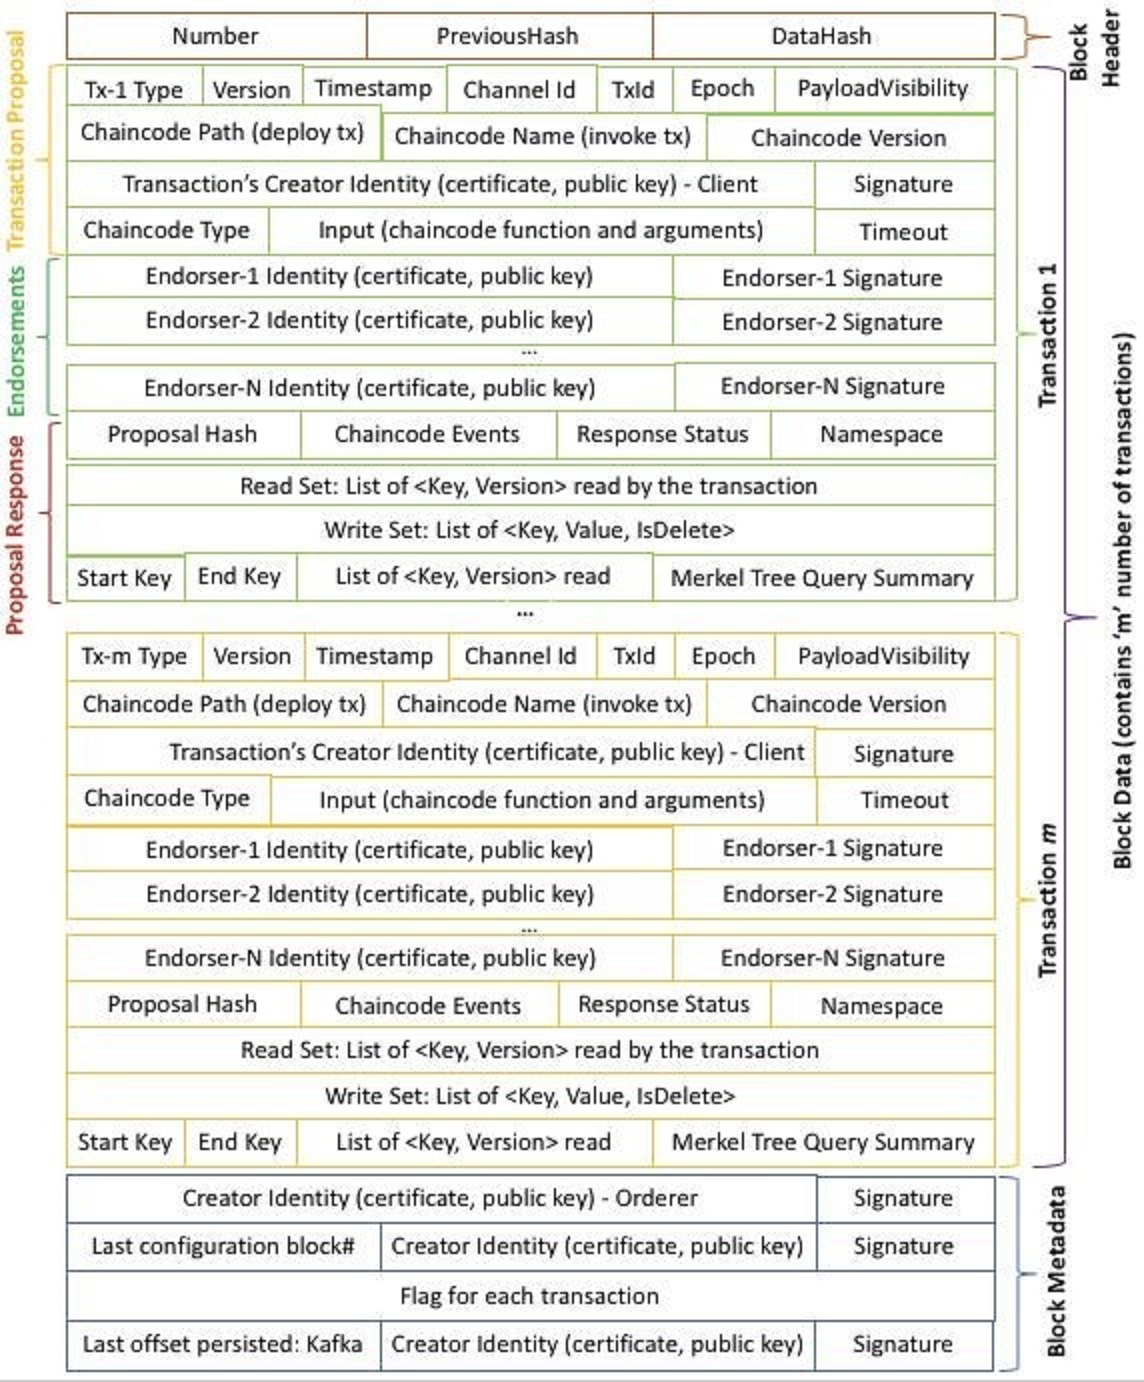
\includegraphics [scale=0.5] {hlf_block_structure}
	\caption{Структура блока Hyperledger Fabric}
	\label{fig:hlf_block_structure}
\end{figure}

\textbf{Сервисная служба (Ordering Service).} Узел сервисной службы (OSN) участвует в консенсусе и составляет блок транзакций, который доставляется узлам по протоколу “сплетни” (gossip protocol). Структура блока в Fabric показана на рисунке \ref{fig:hlf_block_structure}. Сервисная служба является модульной и поддерживает подключаемый механизм консенсуса. По умолчанию последовательное упорядочение (то есть консенсус) достигается с помощью базового кластера Kafka / Zookeeper. OSN публикуют транзакции в темах kafka и используют упорядоченный и неизменный характер записей в темах kafka для создания уникальной упорядоченной последовательности транзакций в блоке. Блок обрезается, когда добавляется максимальное количество новых транзакций с момента последнего среза блока или установленное время ожидания с момента последнего среза блока. Когда какое-либо одно условие удовлетворяется, блок доставляется на равноправные узлы.

\textbf{Клиент (Client).} Клиентское приложение отвечает за составление предложения по транзакции, как показано на рисунке \ref{fig:hlf_tx_route}. Клиент отправляет предложение по транзакции одному или более узлам одновременно для сбора ответов с одобрениями для удовлетворения политики одобрения. Затем он передает транзакцию сервисной службе, которая включит её в блок и доставит всем узлам для проверки и подтверждения. В Fabric ответственность лежит на клиенте, чтобы гарантировать, что транзакция правильно сформирована и удовлетворяет политикам одобрения.
\begin{figure}[ht]
	\centering
	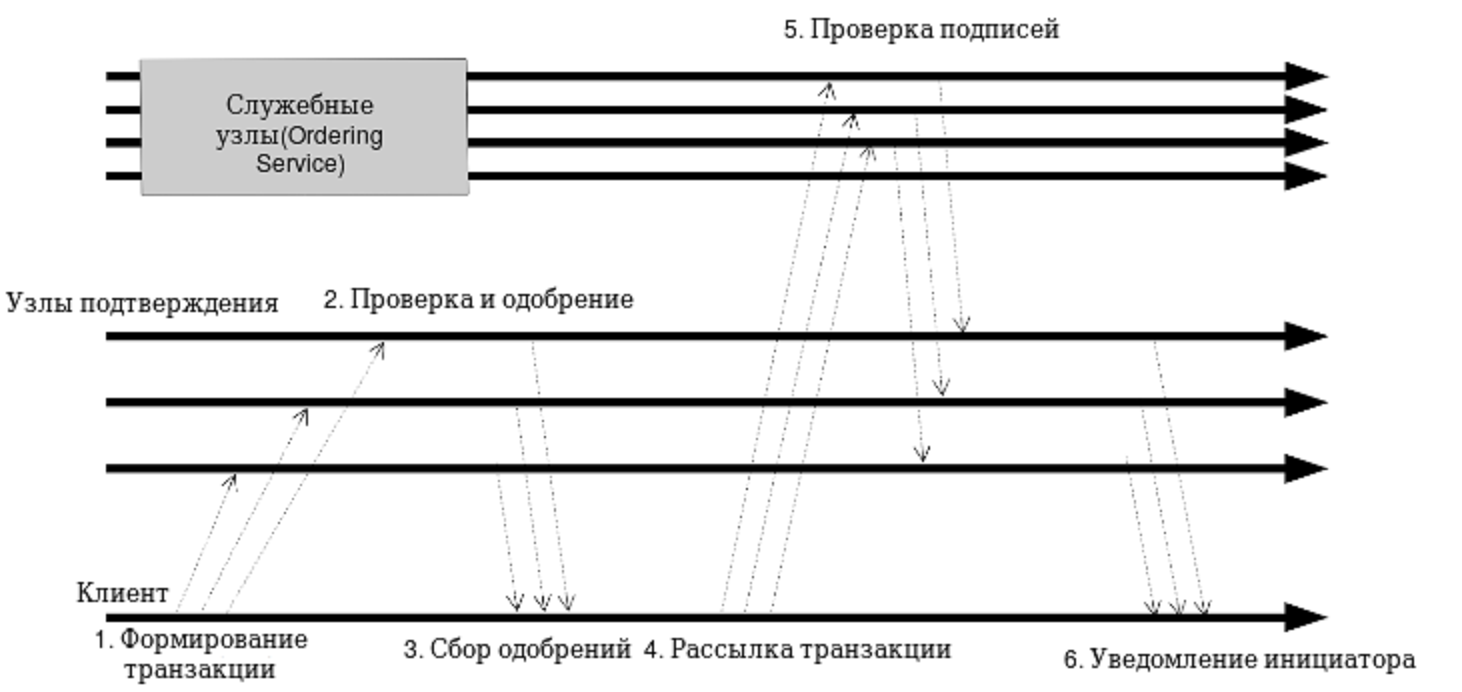
\includegraphics [scale=0.5] {hlf_tx_route}
	\caption{Путь транзакции в Hyperledger Fabric}
	\label{fig:hlf_tx_route}
\end{figure}

\subsubsection{Путь транзакции в Hyperledger Fabric} \label{subsubsec:ch1/sec3/subsec1/subsubsec2}

В отличие от других блокчейн-сетей, в которых используется модель транзакции “order-execute”, в Fabric используется модель “simulate order-validate\& commit”. На рисунке \ref{fig:hlf_tx_route} изображен поток транзакций, который включает в себя 3 этапа:
\begin{itemize}
	\item Фаза одобрения - моделирование транзакции на отдельных участниках и сбор изменений состояния;
	\item Этап	упорядочения	-	упорядочение транзакций по согласованному протоколу;
	\item Этап валидации - валидация с последующей фиксацией в реестре.
\end{itemize}

Прежде чем транзакции могут быть отправлены в Fabric, необходимо загрузить сеть с участвующими организациями, их MSP и идентификаторами для партнеров. Сначала в сети заказчика создается канал с соответствующими MSP организации. Во-вторых, коллеги каждой организации присоединяются к каналу и инициализируют реестр. Наконец, необходимые смарт-контракты устанавливаются на канал.


\textbf{Фаза одобрения (Endorsement Phase).} Клиентское приложение, использующее Fabric SDK создает предложение по транзакции для вызова функций кода, которые, в свою очередь, будут выполнять операции чтения и
/ или записи в состоянии регистра. Предложение подписывается учетными данными клиента, и клиент отправляет его одному или более подтверждающим партнерам одновременно. Политика одобрения для смарт-контракта диктует, каким организациям-партнерам клиент должен отправить предложение для моделирования.

Во-первых, каждый подтверждающий одноранговый узел проверяет, что отправитель уполномочен вызывать транзакции на канале. Во-вторых, одноранговый узел выполняет код, который может получить доступ к текущему состоянию регистра в одноранговом узле. Результаты транзакции включают в себя значение ответа, набор для чтения и набор для записи. Все операции чтения читают текущее состояние регистра, а записи перехватываются и изменяют приватное рабочее пространство транзакции. В-третьих, подтверждающий одноранговый узел вызывает системный код, называемый ESCC, который подписывает этот ответ на транзакцию с идентификатором партнера и отвечает обратно клиенту с ответом на предложение. Наконец, клиент проверяет ответ предложения, чтобы убедиться, что на нем стоит подпись партнера. Клиент собирает достаточное количество ответов на предложения от разных партнеров, проверяет, что одобрения одинаковы. Поскольку каждый узел мог выполнить транзакцию на разной высоте в блокчейне, возможно, что ответ предложения отличается. В таких случаях клиент должен повторно предоставить предложение другим партнерам, чтобы получить достаточные совпадающие ответы.

\textbf{Фаза сервиса (Ordering Phase).} Клиент передает ответы от узлов, осуществляющих одобрение, в виде упакованной транзакции, в которой содержатся идентификаторы и подписи узлов (Endorsers), а также сгенерированные Read Set и Write Set. Read Set - это данные world-state, которые были прочитаны во время симуляции смарт контракта, а Write Set - это те данные, которые подверглись изменению
Узел сервисной службы (Orderer) получает транзакции от разных клиентов для разных каналов и ставит их в очередь для каждого канала. Он создает блоки транзакций для каждого канала, подписывает блок своим ключом и доставляет их партнерам, используя протокол обмена сообщениями.

\textbf{Этап валидации (Validation Phase).} Все одноранговые, как одобряющие, так и фиксирующие узлы на канале, получают блоки из сети. Узел сначала проверяет подпись узла сервиса на блоке. Каждый действительный блок декодируется, и все транзакции в блоке проходят проверку VSCC перед выполнением проверки MVCC.

Проверка	VSCC	оценивает	одобрения	в	транзакции	в		соответствии	с политикой	одобрения,		указанной	для	смарт-контракта.		Если	политика подтверждения не выполняется, то эта транзакция помечается как недействительная. Проверка MVCC. Как следует из названия, проверка Multi-Version Concurrency Control гарантирует, что версии ключей, считанные транзакцией во время фазы подтверждения, совпадают с их текущим состоянием в реестре во время коммита. Это похоже на проверку конфликта чтения-записи, выполняемую для управления параллелизмом, и выполняется последовательно для всех действительных транзакций в блоке (как отмечено проверкой VSCC). Если версии набора для чтения не совпадают, это означает, что предыдущая транзакция изменила прочитанные данные и была (с момента одобрения) успешно принята, транзакция помечается как недействительная. Чтобы убедиться, что фантомных чтений не происходит, для запросов выполняется повторный запрос и сравниваются хэши результатов (которые также сохраняются как часть набора для чтения, полученного во время одобрения).

\textbf{Этап обновления реестра (Ledger Update Phase).} В качестве последнего шага обработки транзакций регистр обновляется путем добавления блока в локальный регистр. StateDB, которая содержит текущее состояние всех ключей, обновляется наборами записей допустимых транзакций (как отмечено валидацией MVCC). Эти обновления для StateDB выполняются атомарно для блока транзакций и применяют обновления, чтобы привести StateDB в актуальное состояние после обработки всех транзакций в блоке.

% BACKAUP END
\section{Триллеммы децентрализованных систем} \label{sec:ch1/sec4}

Главная проблема распределенных архитектур описана в утверждении, общепринято известном как “теорема CAP”. Теорема CAP  утверждает, что в распределенном хранилище данных невозможно гарантировать более двух из трех свойств: согласованность (Consistency), доступность (Availability) и устойчивость к разделению (Partition Tolerance). Распределенное хранилище данных, таким образом, может быть охарактеризовано только двумя свойствами, а именно CA, CP или AP. Схематично данное разделение представлено на рисунке \ref{fig:cap_theoreme}.

\begin{figure}[ht]
	\centering
	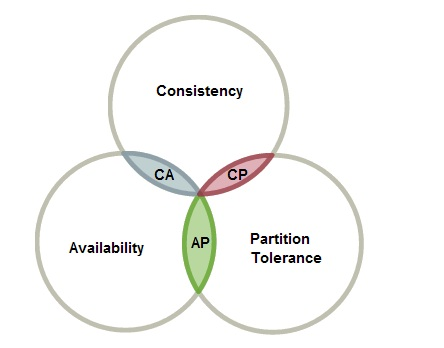
\includegraphics [scale=1.0] {cap-theorem}
	\caption{Теорема CAP}
	\label{fig:cap_theoreme}
\end{figure}

Более конкретно, теорема нацелена на распределенные системы, развернутые через ненадежные сети (сети с ошибками и задержками, такие как Интернет), приводя к разделению компонентов системы. Согласно CAP, в этих средах архитектура системы должна быть ориентирована на баланс между доступностью и последовательность. Например, ACID (атомарность, согласованность, изоляция,
стойкость), обычно предоставляемый RDBMS (реляционной базой данных) гарантирует согласованность на одном узле за счет доступности через несколько узлов (тип CP).

В отличие от этого, Fabric спроектирован так же, как и многие другие блокчейн платформы, как тип AP с возможной согласованностью, также называемой BASE (Basically Available, Soft state, Eventual consistency), при этом такой подход напрямую противопоставляется ACID. Под базовой доступностью подразумевается такой подход к проектированию приложения, чтобы сбой в некоторых узлах приводил к отказу в обслуживании только для незначительной части сессий при сохранении доступности в большинстве случаев. Неустойчивое состояние подразумевает возможность жертвовать долговременным хранением состояния сессий (таких как промежуточные результаты выборок, информация о навигации, контексте), при этом концентрируясь на фиксации только критичных операций. Согласованность в конечном счёте, трактуются как возможность противоречивости данных в некоторых случаях.

В контексте блокчейна, свойства CAP могут быть определены следующим образом:
\begin{itemize}
	\item \textbf{Согласованность:} сеть блокчейн избегает разветвлений цепи.
	\item \textbf{Доступность:} транзакции, представленные клиентами, постоянно записываются в блокчейн и доступны на всех сетевых пирах.
	\item \textbf{Устойчивость к разделению:} сеть блокчейна продолжает работать, несмотря на произвольное количество транзакций или блоков отброшенных (или задерживающихся) в физической сетевой среде между узлами.
\end{itemize}

Fabric реализует свойства CAP следующим образом:
\begin{itemize}
	\item \textbf{Согласованность:} общий порядку транзакций и управление версиями с использованием MVCC.
	\item \textbf{Доступность:} путем размещения копии блокчейна в каждом из пиров.
	\item \textbf{Устойчивость к разделению:} поддерживая работу, несмотря на неисправные узлы (до порогового значения).
\end{itemize}

Из этого следует, что доступность и устойчивость к разделению (свойство AP теоремы) по умолчанию гарантированы в большинстве систем блокчейна. Тем не менее, свойство согласованности обеспечить сложнее.

Fabric достигает согласованности, комбинируя следующие элементы:
\begin{itemize}
	\item Обработка транзакций разбита на последовательность шагов по нескольким компоненты сети.
	\item Клиенты подключаются к каналу связи и отправляют транзакции для одобрения пирами, а только затем к связующим звеньям.
	\item Связующие звенья связывают транзакции в блоки, т.е. порядок транзакций гарантированно согласован по всей сети. Созданные блоки передаются каждому пиру канала. Протокол вещания гарантирует надежную доставку пирам в правильном порядке, а именно, в общем порядке.
	\item При получении блока на узле, равноправный узел использует MVCC для проверки каждой транзакции. MVCC проверка гарантирует согласованность полученного блока и предотвращает атаки, такие как двойные расходы. Тем не менее, это может также привести к устранению других действительных транзакций, которые были отправлены в неправильном порядке. Транзакции помечаются как действительные и недействительные в блокчейне.
	\item Цепь содержит последовательность полностью упорядоченных блоков, где каждый блок содержит последовательность полностью упорядоченных транзакций (действительных или недействительных), что приводит к получению общего порядка по всем транзакциям во всей цепи.
\end{itemize}
 
Теорема САР имеет сходство с трилеммой блокчейна, сформулированной Виталиком Бутерином теоремой о том, что нельзя одновременно достичь идеала по трем параметрам:
\begin{itemize}
	\item Масштабируемость;
	\item Безопасность;
	\item Децентрализация.
\end{itemize}

На рисунке~\ref{fig:trilem-blockchain} цветами отмечены характеристики системы с уклоном в тот или иной параметр:
\begin{itemize}
	\item \textbf{Зеленый:} сбалансированное состояние трех условий;
	\item \textbf{Красный:} сильная безопасность, но ограниченные децентрализация и масштабируемость;
	\item \textbf{Синий:} высокая эффективность, но безопасность и децентрализация ограничены;
	\item \textbf{Черный:} высокая децентрализации, но нет некоторых аспектов масштабируемости и безопасности.
	\item \textbf{Серый:} полная децентрализация, с минимальными или отсутствующими качествами безопасности и масштабируемости.
	\item \textbf{Фиолетовый:} равный баланс между безопасностью и масштабируемостью, отказ от децентрализации.
\end{itemize}

\begin{figure}[ht]
	\centering
	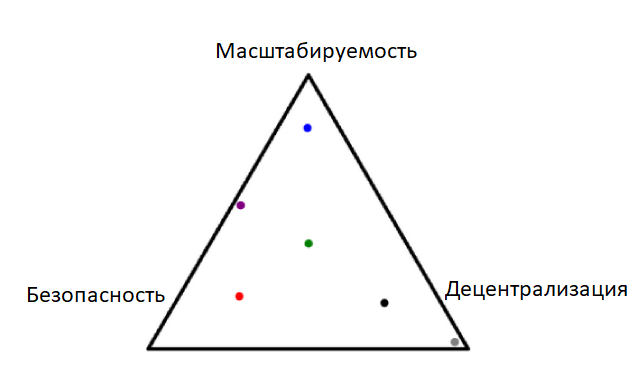
\includegraphics [scale=1.0] {trilem-blockchain}
	\caption{Визуализация трилемммы блокчейна}
	\label{fig:trilem-blockchain}
\end{figure}

Под децентрализацией мы понимаем возможность запускать блокчейн на таких небольших компьютерах, как ноутбуки, сохраняя при этом безопасность даже в случае проведения атаки с превосходящими мощностями. Таким образом поддерживается устойчивость блокчейна к попытке его изменения, одновременно сохраняя возможность быстро и, что немаловажно, одновременно совершать и обрабатывать большое количество (относительно размера сети) транзакций.

В ранних реализациях блокчейна не было уделено должного внимания масштабируемости системы, тогда как в блокчейнах последующих поколения отклоняются от децентрализации в угоду масштабируемости. Не все узлы таких реализаций синхронизируют  свои действия друг с другом, а, например, только некоторое количество самых мощных узлов с высокой пропускной способностью. Так как валидаторов можно сменить путем голосования, сеть всё еще остается децентрализованной. Конечно, 21 компьютер — это не 10 000, как в Биткоине, зато и скорость в среднем достигла 3000 транзакций в секунду.


\section{Постановка задачи} \label{sec:ch1/sec5}
В рамках данной работы требуется реализовать систему электронного документооборота как части инфраструктуры предприятия на примере задачи подписания документов в вузе. Разрабатываемый СЭД должен быть основан на распределенном реестре и иметь клиент в виде мобильного приложения.

Для этого необходимо реализовать следующие задачи:
\begin{enumerate}
	\item Изучить Enterprise-решение Hyperledger Fabric как систему, реализующую технологию распределенных реестров.
	\item Изучить способы построения надежных систем документооборота.
	\item Реализовать бизнес приложение для системы электронного документооборота.
	\item Реализовать интерфейс взаимодействия с бизнес-приложением на основе REST-API.
	\item Реализовать мобильное приложение представляющее возможность взаимодействовать с распределенным реестром посредством графического интерфейса.
\end{enumerate}

Ключевой аспект системы, разработка которой является одной из задач данной работы, - надежность. Этот аспект назван ключевым, так как в области работы с документами высокая защищенность данных является одной из наиболее необходимых характеристик системы. Системы, основанные на блокчейне, по определению имеют хороший уровень безопасности, поэтому в нашем случае цель определяет технологию которую мы используем.           % Глава 1
\chapter{Проектирование программного обеспечения} \label{ch:ch2}
\iffalse % figure sample
\begin{figure}[ht]
	\centering
	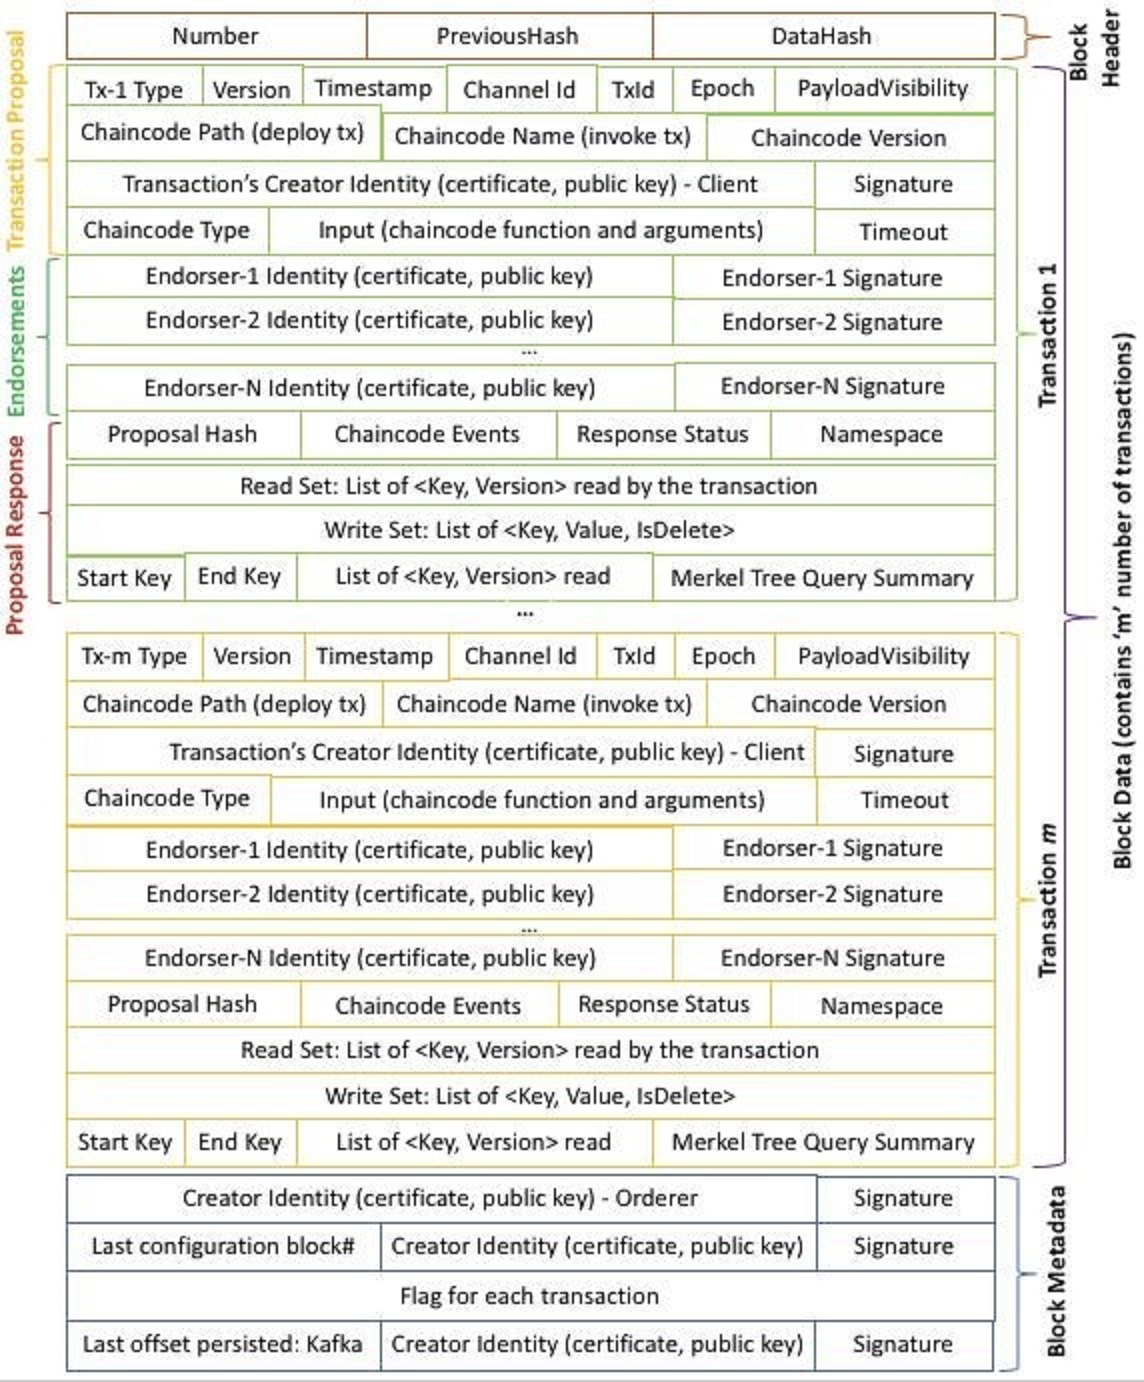
\includegraphics [scale=0.5] {hlf_block_structure}
	\caption{Структура блока Hyperledger Fabric}
	\label{fig:hlf_block_structure}
\end{figure}
\fi
\section{Типичные архитектуры Fabric ориентированных приложений} \label{sec:ch2:sec1}
Приложения взаимодействуют с сетью Hyperledger Fabric посредством SDK по протоколу gRPC как показано на рисунке \ref{fig:apps_use_sdk}. 
Они обращаются к узлам бизнес сети для вызова и/или запроса чейнкода, чтения данных из блокчейна, регистрируют слушателей событий, а так же выполня.т различные административные задачи такие как, запрос и/или изменение конфигурации узлов.
\begin{figure}[ht]
	\centering
	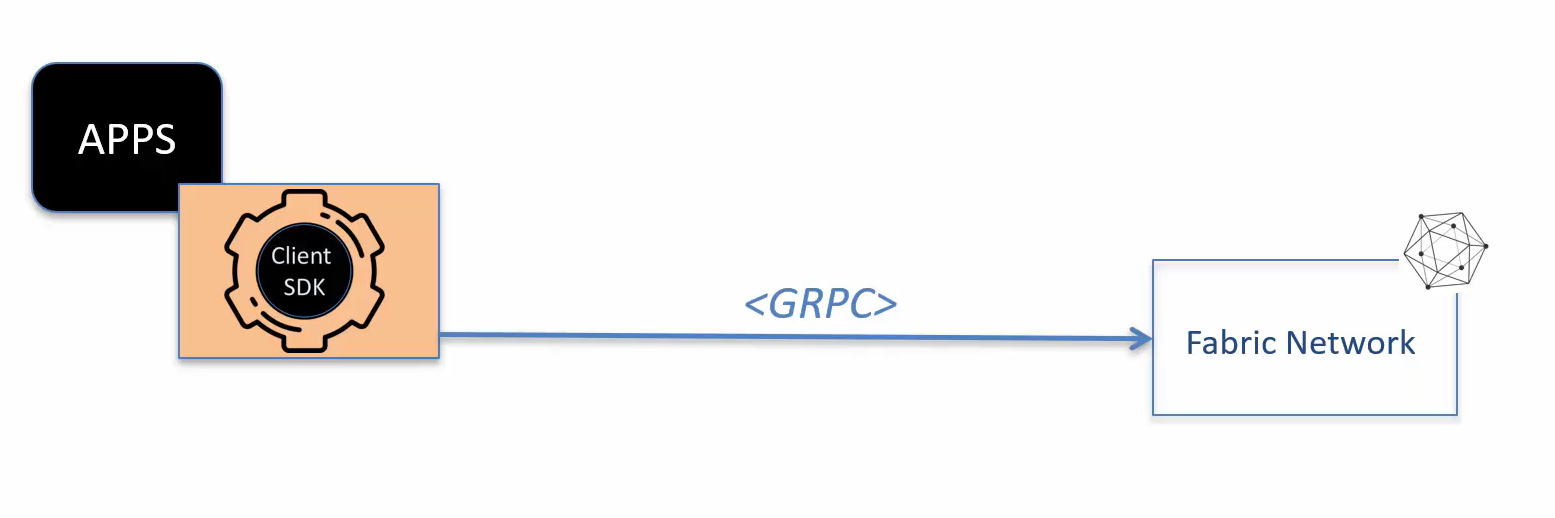
\includegraphics [scale=0.5] {apps_use_sdk}
	\caption{Взаимодействие приложений с Fabric Network}
	\label{fig:apps_use_sdk}
\end{figure}
Как уже упоминалось выше все эти операции осуществляются с помощью Fabric SDK для языков общего назначения. В настоящее время существуют Fabric SDK для языков Java, Go, Python и JavaScript. Так как каждую технологию следует выбирать для тех целей, для которых она подходит лучше всего, то будет справедливым рассмотреть типы Fabric ориентированных приложений. Чаще всего это:
\begin{itemize} 
	\item Графические приложения, позволяющие пользователю выполнять смарт-контракты через графический интерфейс.
	\item Приложения, представляющие отчеты из хранилища данных чейнкода.
	\item Модули интеграции Fabric SDK в уже существующие проекты, для взаимодействия с системами бекенда.
\end{itemize}
При разработки приложения того или иного типа уместно применение соответствующего шаблона архитектуры.
Рассмотрим типичные шаблоны построение Fabric ориентированных приложений.
Настольные приложения - создание и подписание транзакции посходит локально на компьютере пользователя. Такой подход является хорошо защищенным, но имеет недостаток в виде дистрибуции приложения. При внесении правок в приложение, конечный пользователь вынужден в ручную устанавливать обновления на свой компьютер.
\begin{figure}[ht]
	\centering
	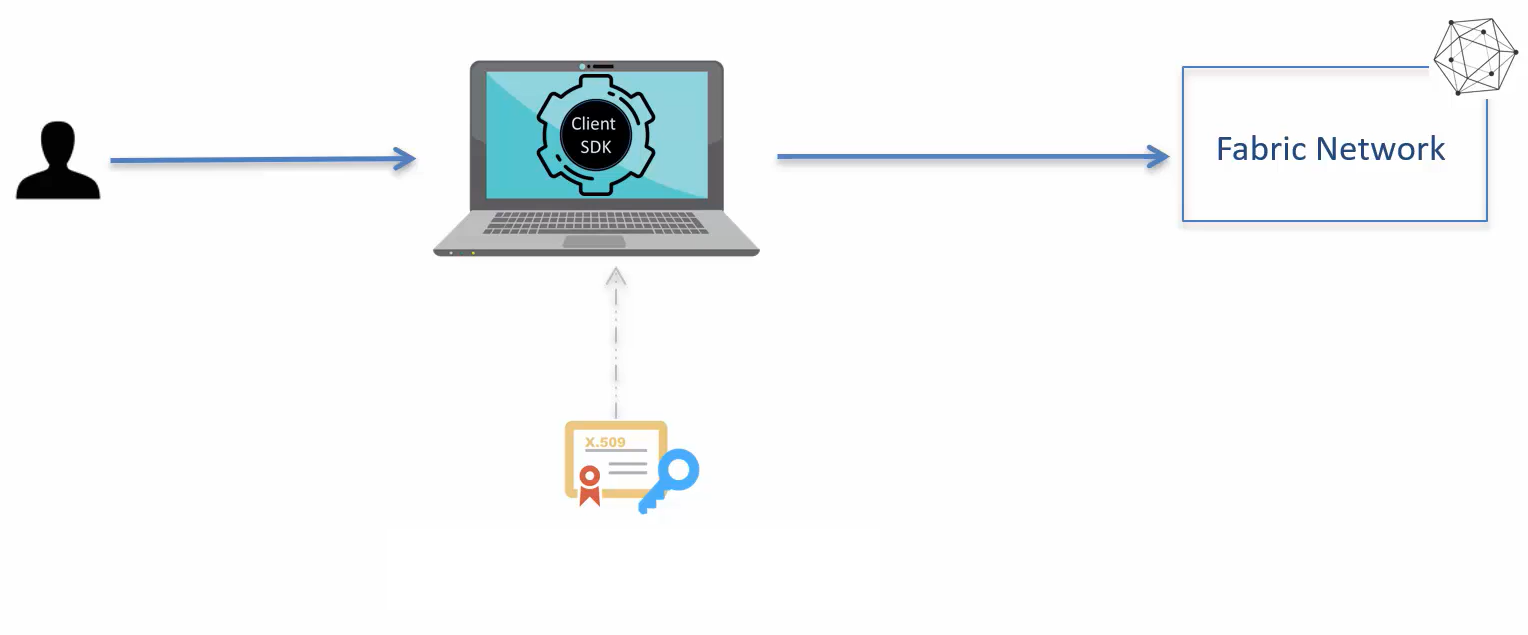
\includegraphics [scale=0.5] {desktop_apps}
	\caption{Настольные приложения, использующие Fabric SDK}
	\label{fig:desktop_apps}
\end{figure}
Обработка транзакций в сети Fabric приводит к возникновению различных событий, которые могут потребляется приложениями. События могут предоставятся клиента посредством некого брокера сообщений (например, Kafka), или же посредством REST-API. При получении определенного события клиентское приложение соответствующим образом обрабатывает его(например, обновляет свои бекенд системы). Так как события инициируются и обрабатываются в режиме реального времени, такой подход широко используется для создания инфопанелей и отчетов в режиме реального времени. Схематично данный шаблон предоставлен на рисунке 
\begin{figure}[ht]
	\centering
	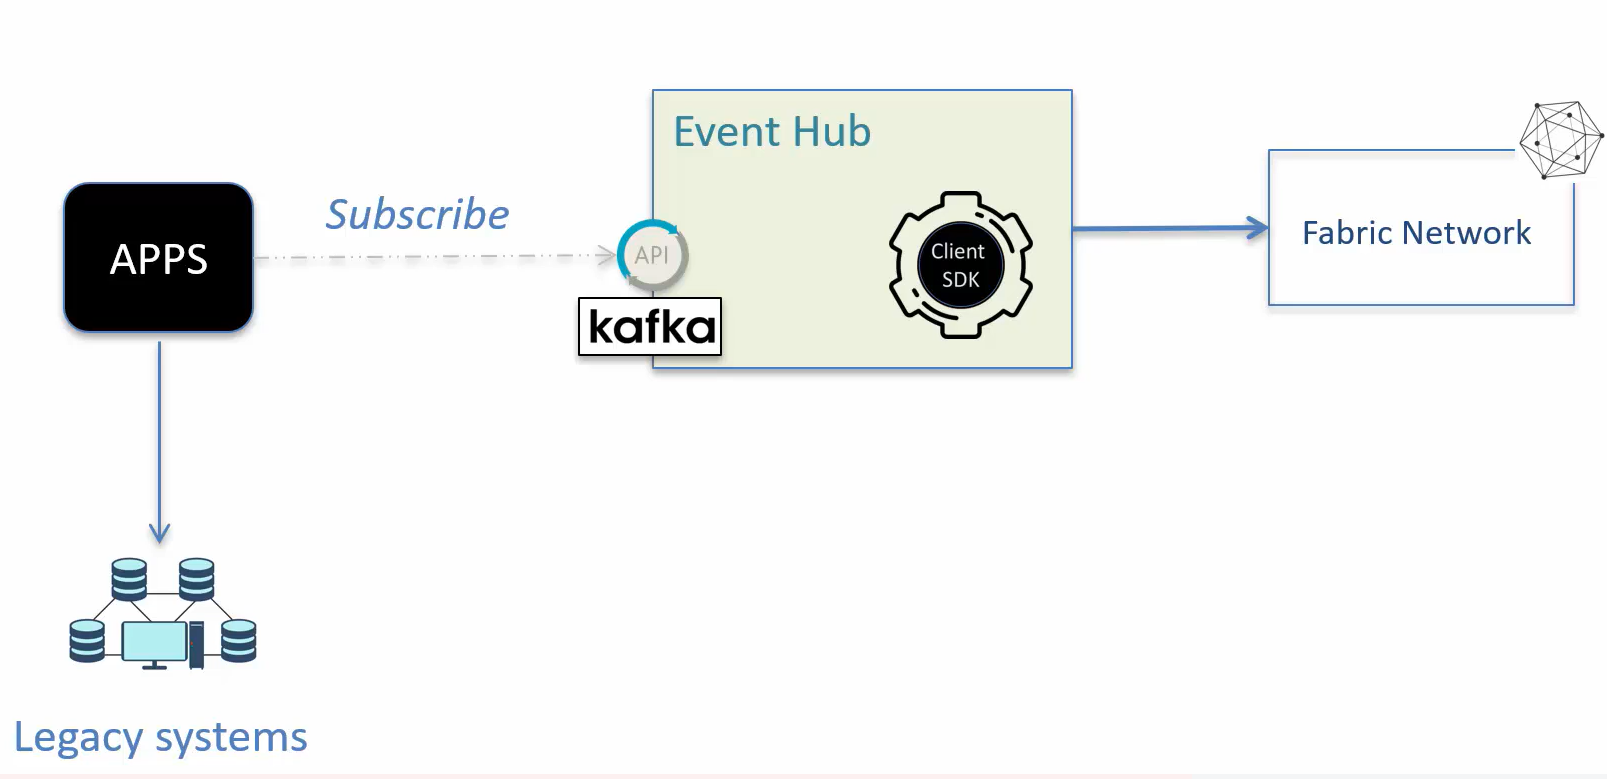
\includegraphics [scale=0.5] {event_hub}
	\caption{Архитектура "Event Hub"}
	\label{fig:event_hub}
\end{figure}
А также Fabric SDK может быть использована для создания различных утилит командной строки. Эти утилиты используется администраторами бизнес сети Hyperledger Fabric для осуществления различных административных задач (Рисунок \ref{fig:admin_cli}).
\begin{figure}[ht]
	\centering
	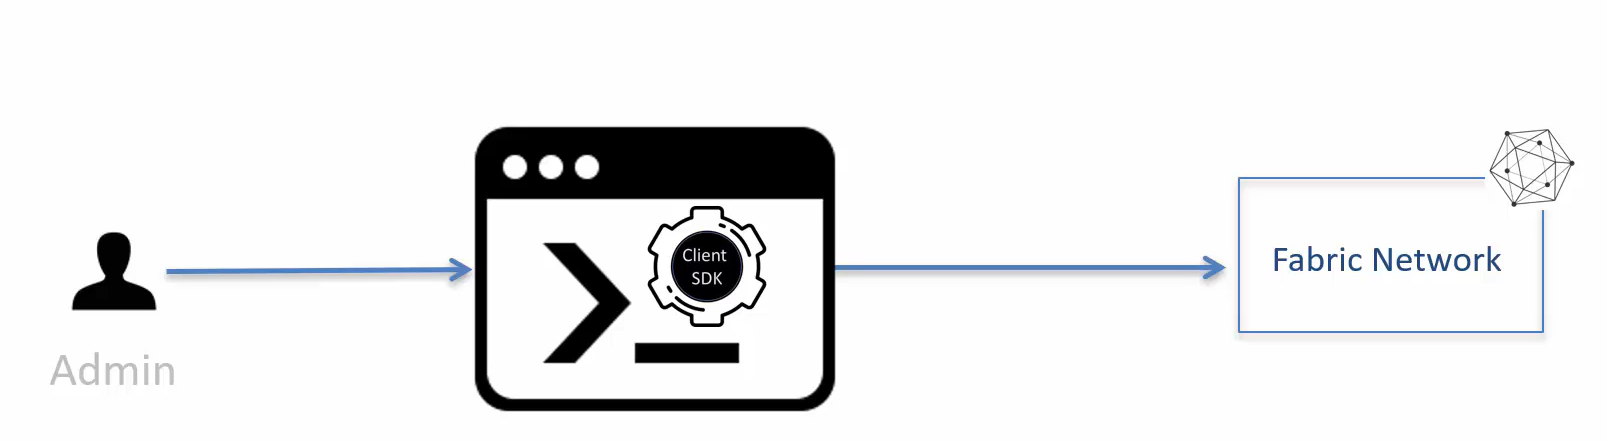
\includegraphics [scale=0.5] {admin_cli}
	\caption{Утилиты командной строки}
	\label{fig:admin_cli}
\end{figure}
Ещё один широк распространенный подход к построению Fabric ориентированных приложений - использование связующего программного обеспечения, ориентированное на обработку сообщений (англ. message-oriented middleware). Это ПО использует Fabric SDK, и обеспечивает связь среды выполнения Fabric с клиентским приложением. Middleware предоставляет API, обращаясь к которому клиентские приложения взаимодействуют с бизнес сетью. При этом тип клиентского приложения может быть любым(настольное, мобильное, веб и д.р.). Cхема такой архитектуры представлена на рисунке
\begin{figure}[ht]
	\centering
	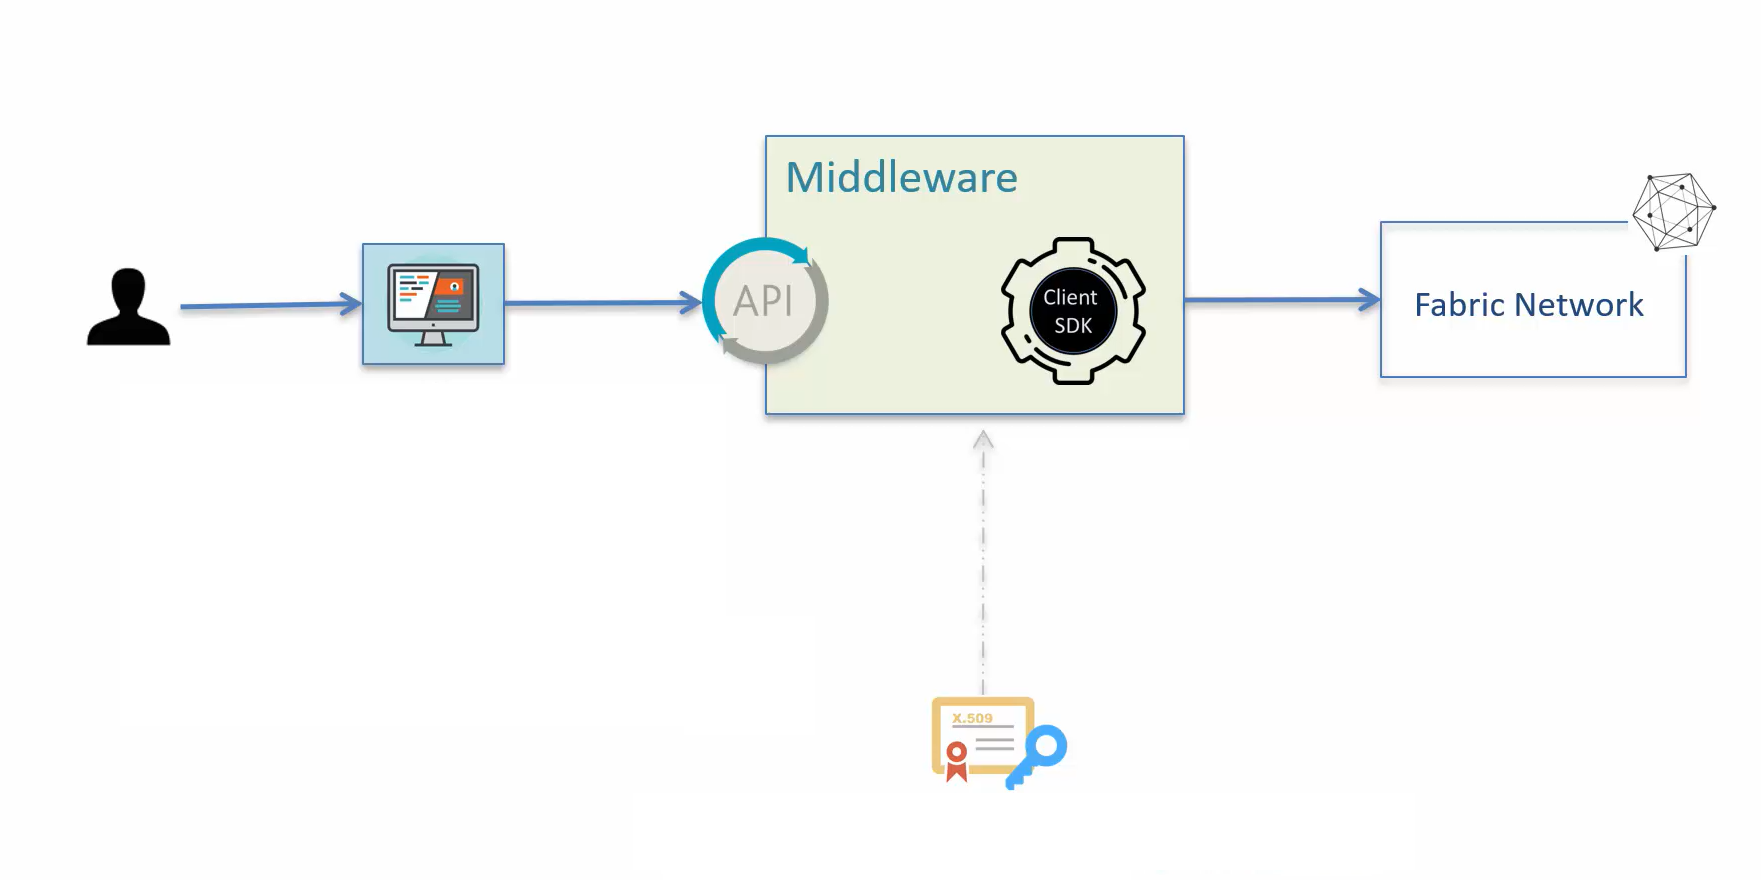
\includegraphics [scale=0.5] {middleware}
	\caption{Архитектура со связующим ПО}
	\label{fig:middleware}
\end{figure}
Но при реализации такого подход возникает ряд вопросов, и первый из них где управлять ключами и сертификатами пользователей? Один из вариантов - управлять ими на стороне middleware. Однако в этом случае пользователи должны доверять хосту middleware, т.к. их приватные ключи оседают на его стороне. Однако в некоторых случаях пользователи могут не доверять организации, осуществляющей хостинг middleware. В таких случаях необходимо закладывать логику работы с приватными ключами и сертификатами на стороне клиентского приложения. Очевидно, что такой подход является более защищенным, однако он так же имеет недостаток в виде увлечения сложности приложения. А также в этом случае нарушается принцип единственной ответственности (SRP). \cite{solid}


	%\section{Обеспечение безопасности REST-сервера} %\label{sec:ch2:sec2}
	%Как миниммум юзать TLS/HTTPs и аутентификацию.

\section{Выбор инструментов и технологий} \label{sec:ch2:sec2}
\subsection{Архитектура} \label{subsec:ch2/sec2/subsec1}
В \ref{sec:ch2:sec1} мы рассмотрели типичные архитектуры  Fabric ориентированных приложений. В данной работе выбор пал на архитектуру со связующим ПО с инкапсуляцией логики работы сертификатами пользователей на стороне связующего ПО. В представленных в работе сценариях отношение между отдельными элементами доверительные, поэтому недостаток данного подхода не создает проблем. К очевидными плюсам данной архитектуры можно, также отнести легкую замену графического клиентского приложения, т.к. ему неизвестно существование бизнес сети, оно работает исключительно со связующим ПО по технологии RPC. \cite{grpc}
На рисунке \ref{fig:sys_architecture} представлена схема архитектуры разработанного приложения.
\begin{figure}[ht]
	\centering
	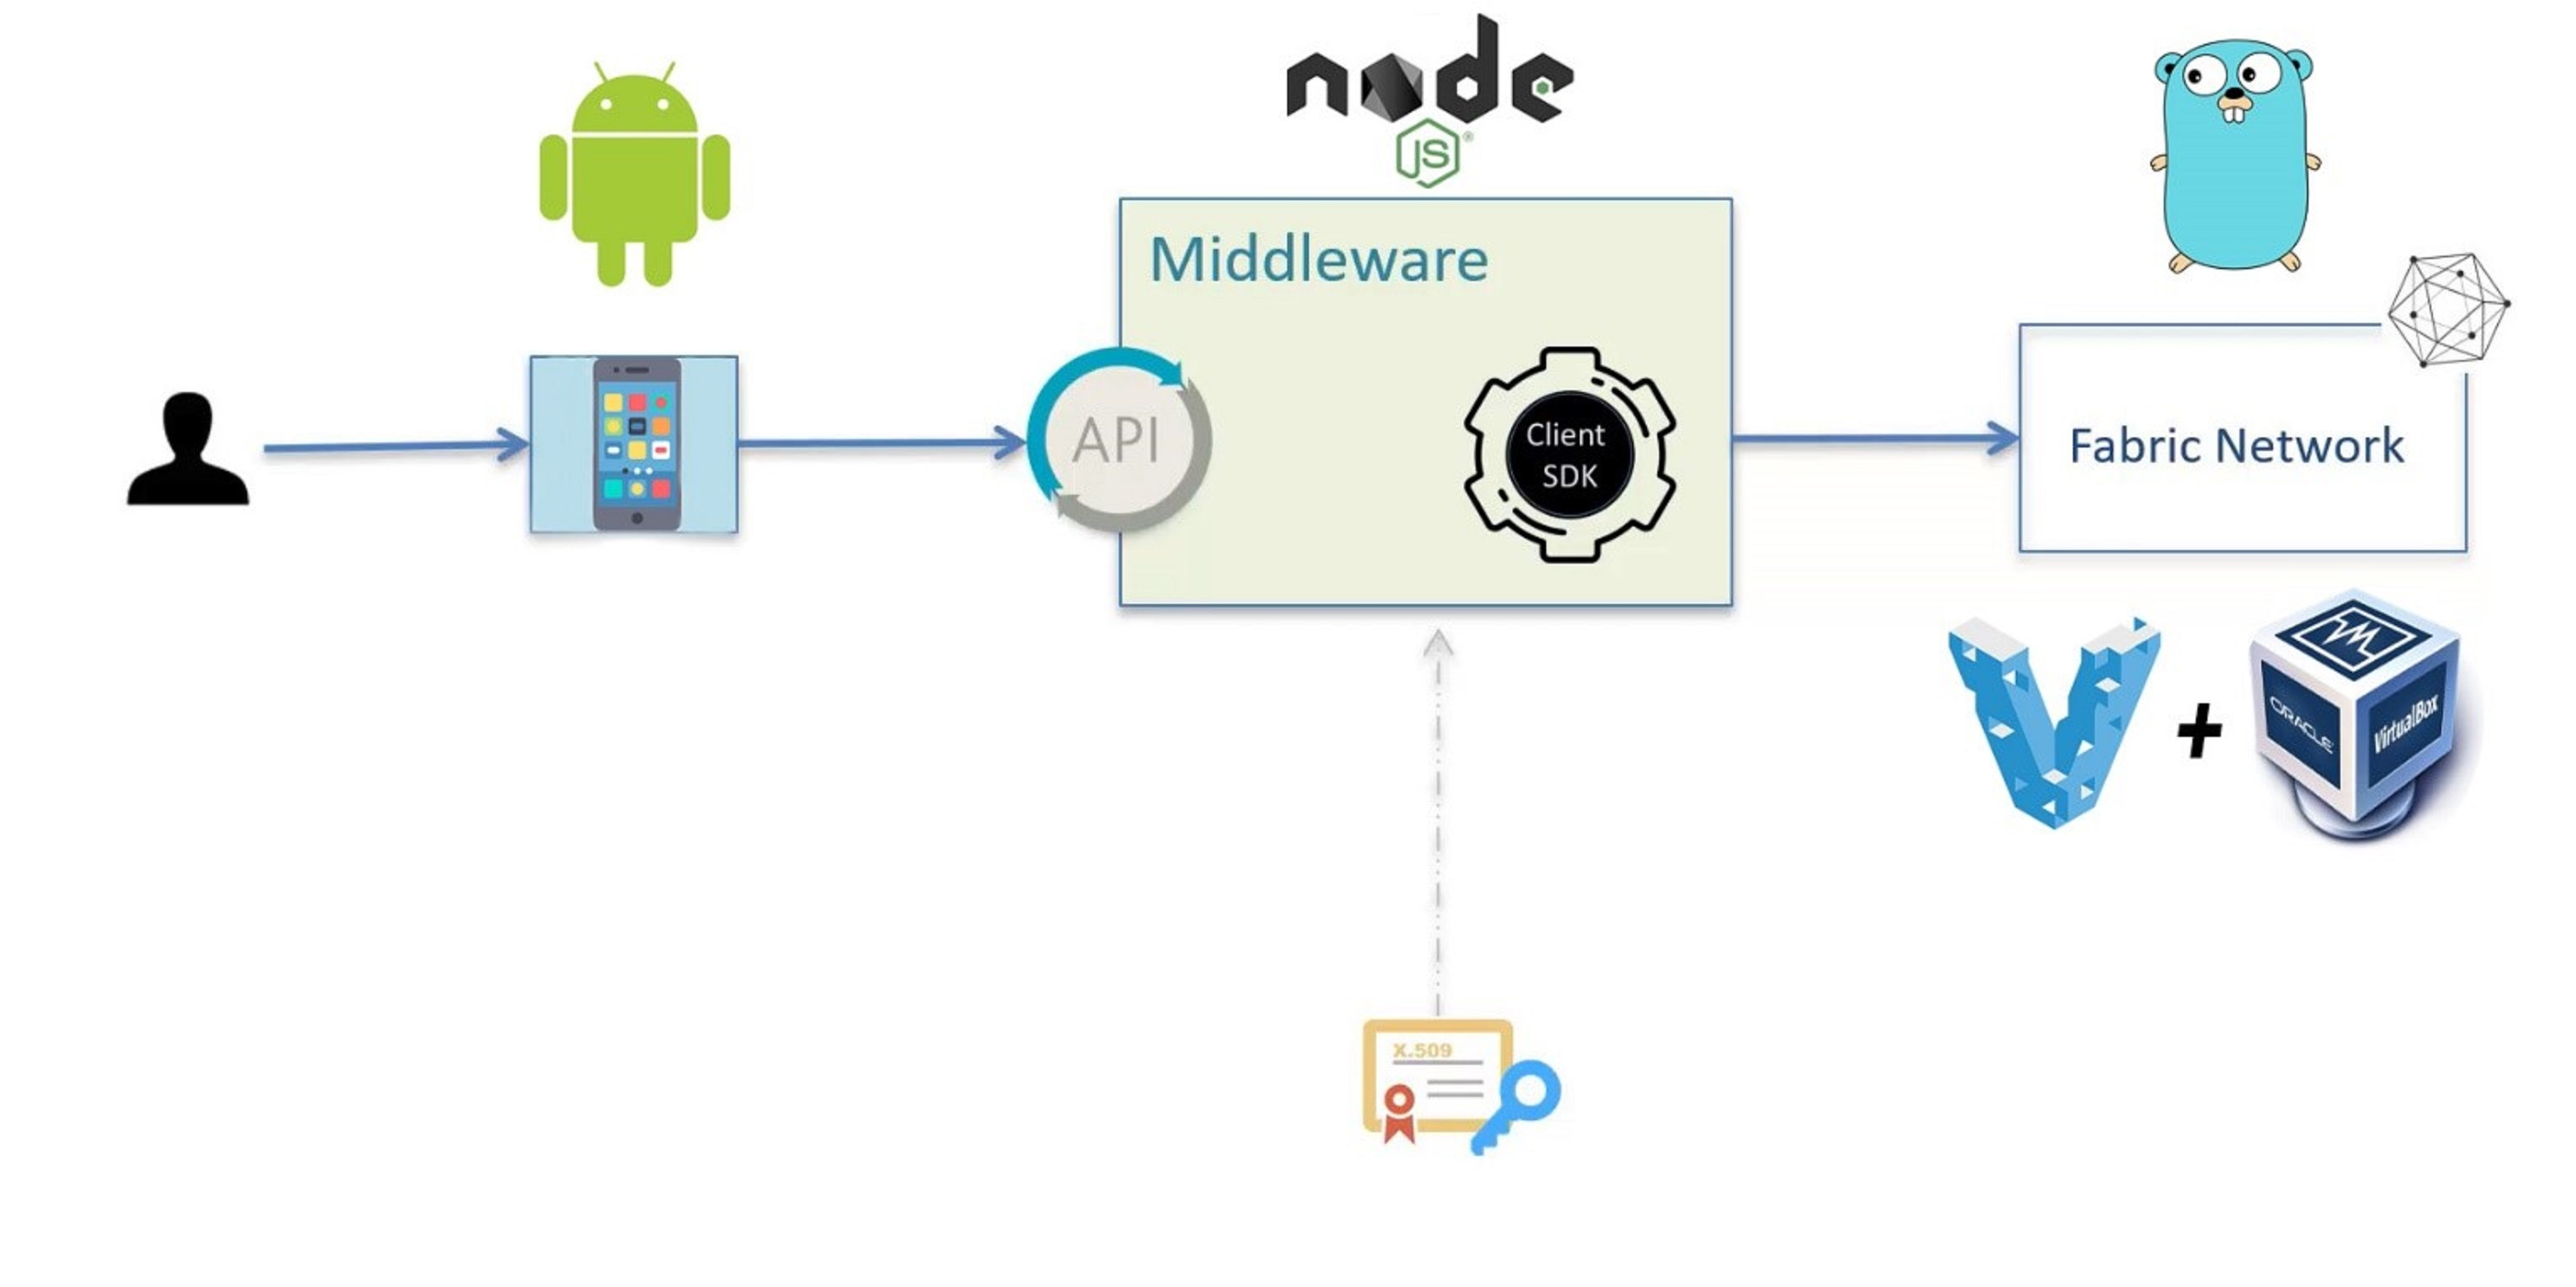
\includegraphics [scale=0.5] {sys_architecture}
	\caption{Архитектура разработанного приложения.}
	\label{fig:sys_architecture}
\end{figure}

\subsection{Смарт контракты} \label{subsec:ch2/sec2/subsec2}

 Есть СДК на нескольких языках, у нас на языке Go почему? ПОТОМУЧТО
 
\subsection{REST-сервер} \label{subsec:ch2/sec2/subsec3}
Для обеспечения связи клиентского приложение со связующим ПО в качестве методологии RPC был выбран REST (Representational State Transfer — передача состояния представления)\cite{restful} Философия этого подхода заключается в том, что приложения моделируются как набор ресурсов, с которыми клиенты могут взаимодействовать (считывать данные, обновлять, удалять и т.д.). В наше время построение приложений с помощью архитектурного стиля REST вкупе с HTTP и JSON\cite{js-json} стало фактическим стандартом для создания микросервисов.
Как уже упоминалось в \ref{sec:ch2:sec1}, Fabric SDK существует для нескольких языков программирования общего назначения, среди которых присутствует JavaScript \cite{pure-js}. 
TODO: Node js\cite{node-js}, npm, express

\subsection{Клиентское приложение}
 \label{subsec:ch2/sec2/subsec3}
 
Т.К. мобильное приложение, а самый распространенная система Андроид то конечно же джава
\iffalse
	Современные приложения редко работают в изоляции. Большинство из них общаются друг с другом по сети и координируют свои действия, обмениваясь сообщениями. Таким образом, современная программная система представляет собой набор распределенных приложений, которые работают на разных участках сети и взаимодействуют с помощью различных коммуникационных протоколов. Например, интернет-магазин может состоять из нескольких распределенных компонентов, таких как система управления заказами, каталог, база данных и т. д. Для реализации бизнес-возможностей подобного интернет-магазина необходимо наладить связь между этими компонентам.
	
	С появлением микросервисной и облачно-ориентированной архитектур традиционные приложения, обладающие разными бизнес-возможностями, подверглись разделению на более мелкие, автономные и бизнес-ориентированные сущности, известные как микро- сервисы. И эти микросервисы должны связываться друг с другом по сети, используя методики межпроцессного (межсервисного, межпрограммного) взаимодействия (inter-process communication, IPC). Существует несколько методик для осуществления межсервисного взаимодествия такие как SOAP, REST, RPC и другие. В данной работе выбор пал на методику REST, так как в наше время построение приложений с помощью архитектурного стиля REST вкупе с HTTP и JSON стало фактическим стандартом для создания микросервисов.  На рисунке \ref{fig:sys_architecture} показана архитектура разработанной системы, где Fabric Network и Middleware рассматриваются как отдельные микросервисы, взаимодействующие друг с другом. Все виды взаимодействий инициируются клиентом.
\fi
           % Глава 2
\chapter{Реализация программного обеспечения} \label{ch:ch3}
\section{Топология blockchain сети} \label{sec:ch3:sec1}
Для развертки сети для разработки используются утилиты командной строки, входящие в дистрибутив Hyperledger Fabric. Большинство из них читают некоторую конфигурацию и запускают соответствующее ПО в контейнерах, образуя узлы сети. Топология сети для разработки представлена на рисунке \ref{fig:network-topology}. Она состоит из 2 обычных узлов и 1 узла сервисной службы. Обычные узлы  владеют своей собственной базой данных Coachdb, хранящей локальную копию блокчейна.

\begin{figure}[ht]
	\centering
	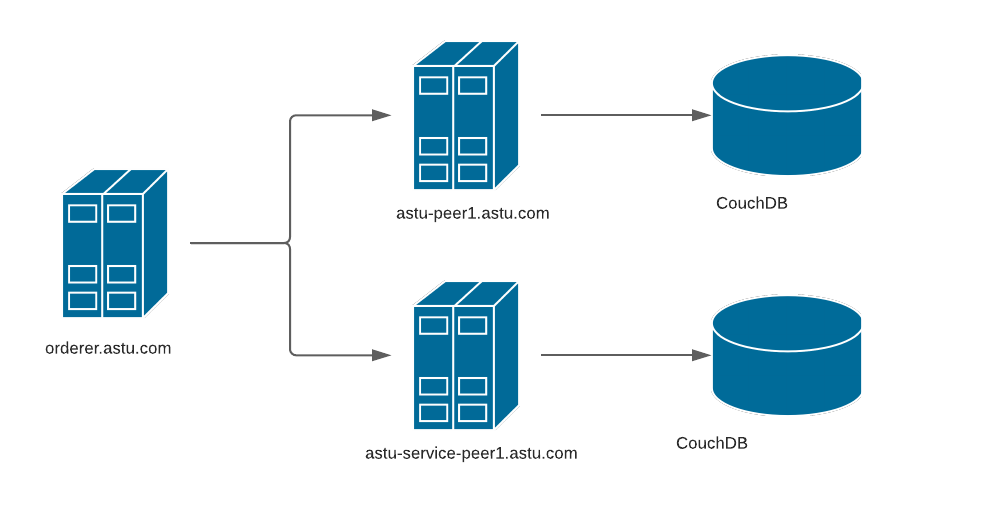
\includegraphics [scale=1.0] {network-topology}
	\caption{Топология сети Fabric, участвовавшая в разработке.}
	\label{fig:network-topology}
\end{figure}

Также существуют конфигурации для подключения к удаленной среде Fabric. В них описывается структура сети, такие элементы, как каналы, узлы, огранизации и т.д. Предназначение этих конфигураций заключается в описании существующей сети Fabric SDK для успешной её работы. Пример конфигурации используемой сервером для подключения к сети, предназначенной для разработки и отладки смарт контрактов представлен на рисунке \ref{fig:dev-network-connection}.

\begin{figure}[H]
	\centering
	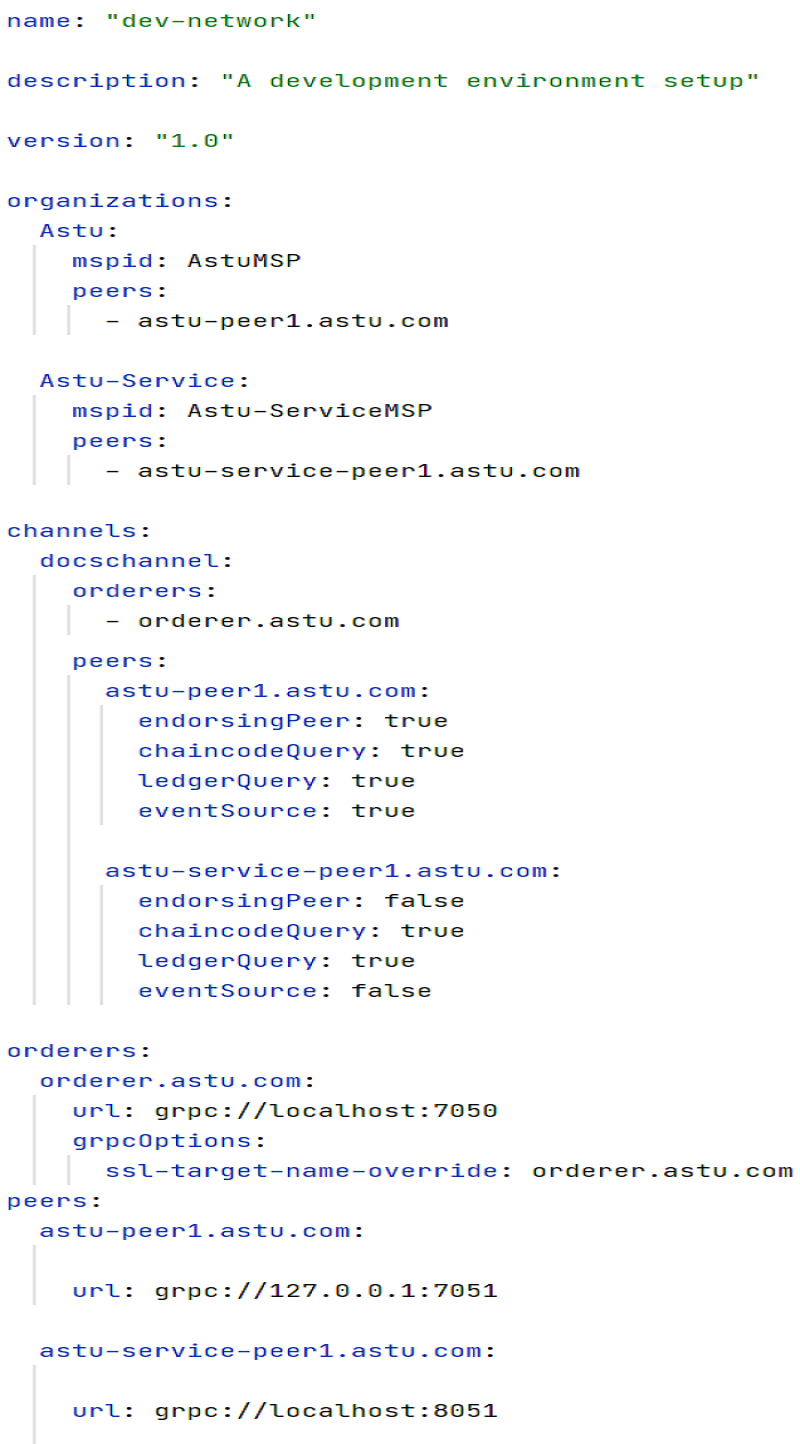
\includegraphics [scale=0.8] {dev-network-connection}
	\caption{Конфигурация подключения к сети Fabric.}
	\label{fig:dev-network-connection}
\end{figure}

\section{Серверная часть} \label{sec:ch3:sec2}

Серверная часть документооборота написана на платформе Node.js с использованием языка JavaScript. Благодаря этой платформе скриптовый язык  JavaScript можно использовать в качестве универсального языка программирования. На рисунке \ref{fig:server-architecture} представлена архитектура серверной части.

\begin{figure}[ht]
	\centering
	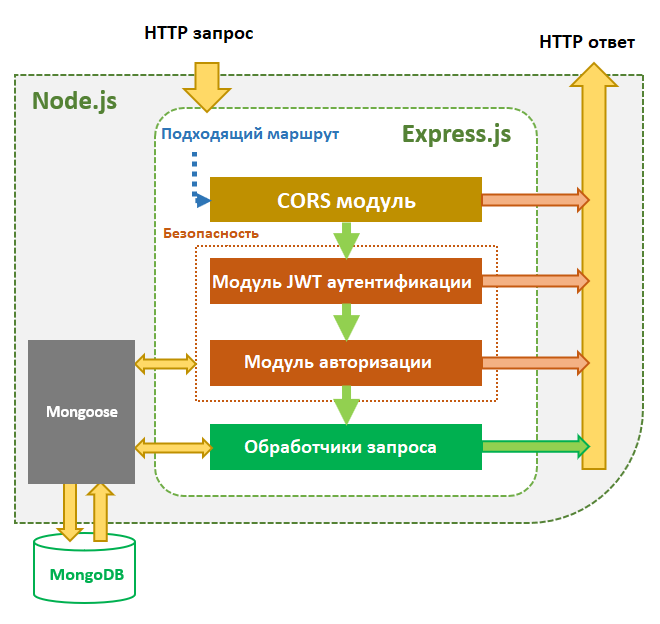
\includegraphics [scale=1.0] {node-js-rus}
	\caption{Архитектура серверной части.}
	\label{fig:server-architecture}
\end{figure}

Сервер предоставляет внешние API, которые могут быть вызваны клиентскими приложениями. Логику API реализуют контроллеры из рисунка \ref{fig:server-architecture}.  

Логически API поделены на 3 группы:
\begin{itemize}
	\item \textbf{Аутентификации и авторизации (АА)} - \textit{/api/auth/**}  - используются для регистрации и авторизации участников документооборота;
	\item \textbf{Сервиса} - \textit{/api/service/**} - используются для представления клиентам информации о структуре возможных документов;
	\item \textbf{Смарт контрактов} - \textit{/api/chaincode/**} - используются для обращение к среде выполнения Fabric с целью исполнения смарт контрактов посредством Fabric SDK.
\end{itemize}

\subsection{Поддержка документов разных типов} \label{subsec:ch3/sec1/subsec1}

Почти любой документ должен соответствовать некоторым стандартам и положениям. Из этого вытекает, то, что структура некоторых документов будет повторяться в зависимости от его типа. Для того чтобы пользователи разработанной системы не были вынуждены производить рутинное написание одних и тех же текстовых содержаний документа (отличающимися лишь некоторыми данными), система документооборота должна поддерживать типизацию документов, которая заключается в хранении атрибутов документа и динамической генерации текстовой составляющей документа. Реализован данный механизм следующим образом: в файловой системе сервера хранятся конфигурации формы для ввода атрибутов текста в формате json, которые подвергается разбору со стороны клиентского приложения и используются им для динамического построения форм ввода атрибутов документов. Пример такой конфигурации для документов типа General представлен в листинге \ref{lst:form-config-general}.

\begin{lstlisting}[caption={Json-конфигурация формы по извлечению аттрибутов документа типа General},label={lst:form-config-general},language=JavaScript]
[
{
	"_id": "title_hint",
	"text": "Название документа",
	"type": 1
},
{
	"_id": "title",
	"is_required": true,
	"hint": "Название документа",
	"type": 2
},
{
	"_id": "content_hint",
	"text": "Текст документа",
	"type": 1
},
{
	"_id": "content",
	"is_required": true,
	"max_length": 7,
	"hint": "Текст документа",
	"type": 12
},
{
	"_id": "signs",
	"hint": "Выберите подписи",
	"text": "Подписи",
	"list": [
	
	],
	"type": 11
},
{
	"_id": "submit",
	"text": "Ок",
	"type": 10
}
]
\end{lstlisting}

Как видно из листинга \ref{lst:form-config-general}, конфигурация формы представляет из себя json массив объектов, служащих для описания элементов интерфейса формы, посредством которой происходит ввод атрибутов документа. Среди атрибутов есть как не уникальные (такие, например, как название и список подписантов) как и уникальные для некоторого типа (например, список студентов и тип практики, если речь идет о приказе о направлении на практику). В листинге \ref{lst:form-config-general} уникальным для своего типа является атрибут content. Он представляет из себя текст документа, который может быть абсолютно любым, данный тип существует для создания неизвестных до некоторого момента типов документов, либо с еще не зафиксированной структурой. Впоследствии такой документ можно будет типизировать в разработанной системе без особых усилий со стороны разработчика. Необходимо будет добавить конфигурацию формы, разработав структуру его атрибутов, и шаблон текстовой составляющей документа. Шаблон представляет из себя текстовый файл с внедренными в него участками JavaScript кода, оперирующего атрибутами документа. При запросе документа на сервере производится замена всех участков кода на значения выполненных выражений. Пример такого шаблона приведен на рисунке \ref{fig:doc-template-practice-permission}.
\begin{figure}[H]
	\centering
	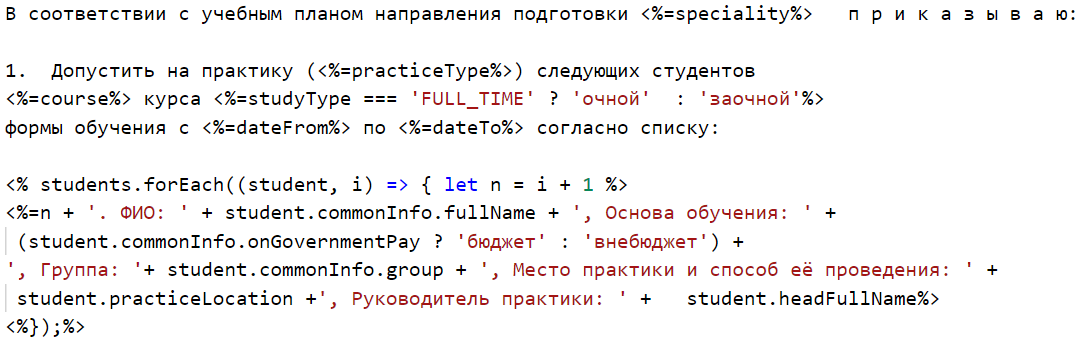
\includegraphics [scale=0.9] {doc-template-practice-permission}
	\caption{Шаблон текстовой составляющей документа типа PracticePermission}
	\label{fig:doc-template-practice-permission}
\end{figure}

Также стоит отметить, что при реализованном устройстве представления текстового содержимого документа, один и тот же документ может быть предоставлен пользователю по разному, для этого достаточно поменять (или изменить) шаблон типа документа. А также, разделение сущности документа на представление и хранимые атрибуты делает удобным восприятие документов различными системами, помимо разработанного клиентского приложения. К таким системам можно отнести дашборды и обозреватели документооборота, которые могут быть интегрированы с разработанным СЭД.
 
\subsection{Описание методов веб-API} \label{subsec:ch3/sec1/subsec2}

В таблице~\ref{tab:apis} представлены маршруты внешних АПИ серверной части приложения, сгруппированные по назначению, как упоминалось в \ref{sec:ch3:sec1}.
\begin{longtable} {| p{8.3cm} | p{8.35cm}l |}
	\caption{Список API серверной части}
	\label{tab:apis}\\
	\hline
	\centering Наименование &  \centering Описание & \\
	\hline
	\multicolumn{2}{|c}{\textbf{API сервиса}} & \\
	\hline
	\endfirsthead
	\caption*{Продолжение таблицы \ref{tab:apis}}\\
	\hline
	\centering Наименование &  \centering Описание & \\
	\hline
	\endhead
	\hline
	\endfoot
	/api/service/getFormConfig (POST) & Получение конфигурации формы для документа определенного типа. &\\
	\hline
	/api/service/getDocTypes (POST) & Получение поддерживаемых типов документов &\\
	\hline
	\multicolumn{2}{|c}{\textbf{API аутентификации и авторизации}} & \\
	\hline
	/api/auth/signIn (POST) & Вход в систему участника документооброта по логину и паролю. &\\
	\hline
	\multicolumn{2}{|c}{\textbf{API смарт контрактов}} & \\
	\hline
	/api/chaincode/newDoc (POST) & Создание нового документа в системе документооброта. &\\
	\hline
	/api/chaincode/getDocs (POST) &Получение списка документов для некоторой группы пользователей &\\
	\hline
	/api/chaincode/changeDoc (POST) & Изменение состояния (одобрение, отклонение, редактирование) существующего документа &\\
\end{longtable}

На рисунках \ref{fig:api-first}-\ref{fig:api-last} приведены диаграммы, описывающие API из таблицы \ref{tab:apis}.

\begin{figure}[H]
	\centering
	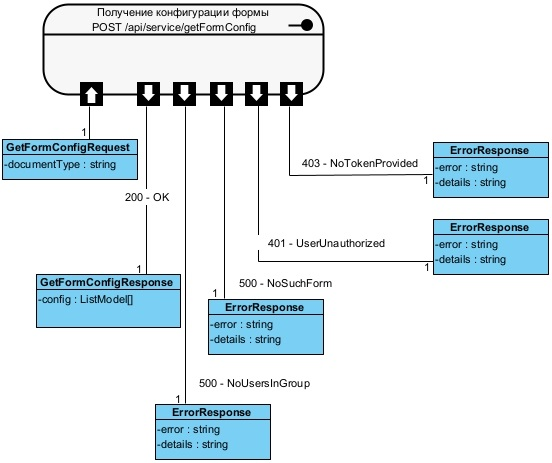
\includegraphics [scale=1.0] {api-getFormConfig}
	\caption{Диаграмма /api/service/getFormConfig.}
	\label{fig:api-first}
\end{figure}

\begin{figure}[H]
	\centering
	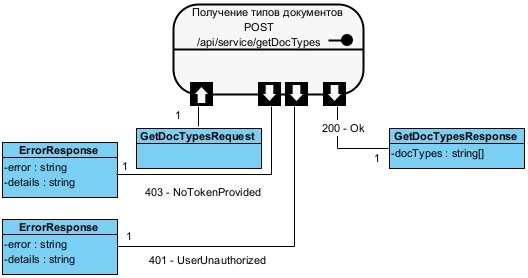
\includegraphics [scale=1.0] {api-getDocTypes}
	\caption{Диаграмма /api/service/getDocTypes.}
	\label{fig:api-getDocTypes}
\end{figure}

\begin{figure}[H]
	\centering
	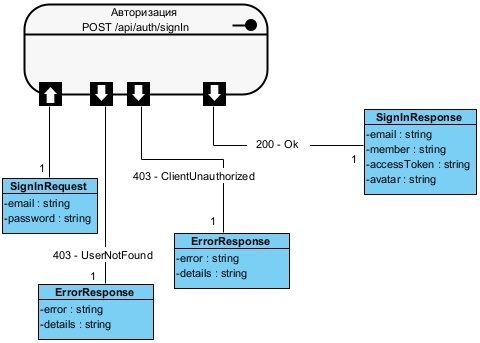
\includegraphics [scale=1.0] {api-signIn}
	\caption{Диаграмма /api/service/getFormConfig.}
	\label{fig:api-signIn}
\end{figure}

\begin{figure}[H]
	\centering
	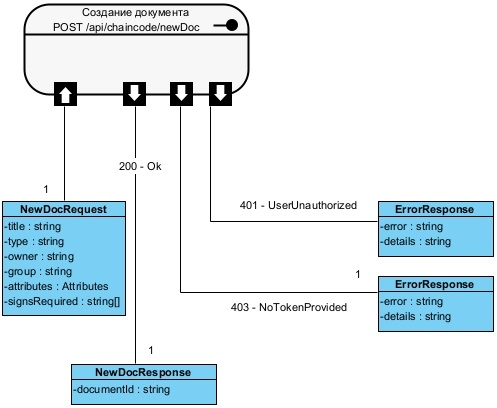
\includegraphics [scale=1.0] {api-newDoc}
	\caption{Диаграмма /api/service/getFormConfig.}
	\label{fig:api-newDoc}
\end{figure}

\begin{figure}[H]
	\centering
	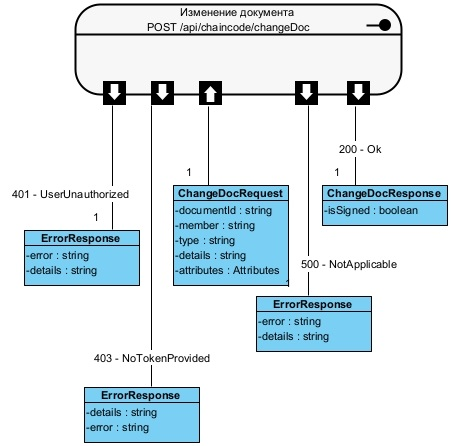
\includegraphics [scale=1.0] {api-changeDoc}
	\caption{Диаграмма /api/service/getFormConfig.}
	\label{fig:api-changeDoc}
\end{figure}

\begin{figure}[H]
	\centering
	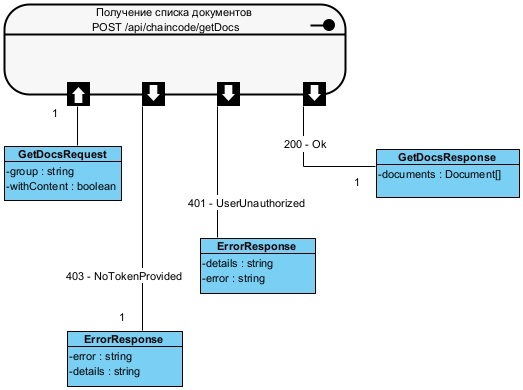
\includegraphics [scale=1.0] {api-getDocs}
	\caption{Диаграмма /api/chaincode/getDocs.}
	\label{fig:api-last}
\end{figure}

\section{Клиентская часть} \label{sec:ch3:sec3}

При реализации клиентского приложения использовался шаблон проектирования архитектуры мобильных приложений MVVVM (Model-View-ViewModel) \cite{anrdoid}.

\begin{figure}[ht]
	\centering
	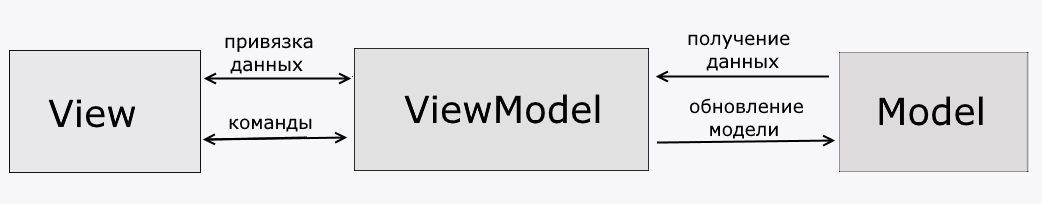
\includegraphics [scale=0.4] {mvvm}
	\caption{Архитектура MVVM.}
	\label{fig:mvvm}
\end{figure}

Такой подход к проектированию архитектуры позволяет разделить представление данных от их модели, что облегчает разработку приложения. А также он позволяет эффективно работать со "связыванием данных", осуществляющее двусторонние связывание данных с визуальными элементами интерфейса. Эта механика, в свою очередь, основана на шаблоне проектирования "Наблюдатель", т.е. при изменение состояние какого либо объекта происходит вызов функций обратного вызова подписчиков. В нашем случае интерфейс и данные являются подписчиками и наблюдателями друг друга.

\subsection{Диаграммы классов} \label{subsec:ch3/sec2/subsec2}
На рисунке \ref{fig:MiddlewareClientNoPackage} изображена диаграмма классов модуля-потребителя API. На рисунке \ref{fig:UiNoPackageRotated} изображена диаграмма классов, отвечающих за работу графического интерфейса.
\begin{figure}[H]
	\centering
	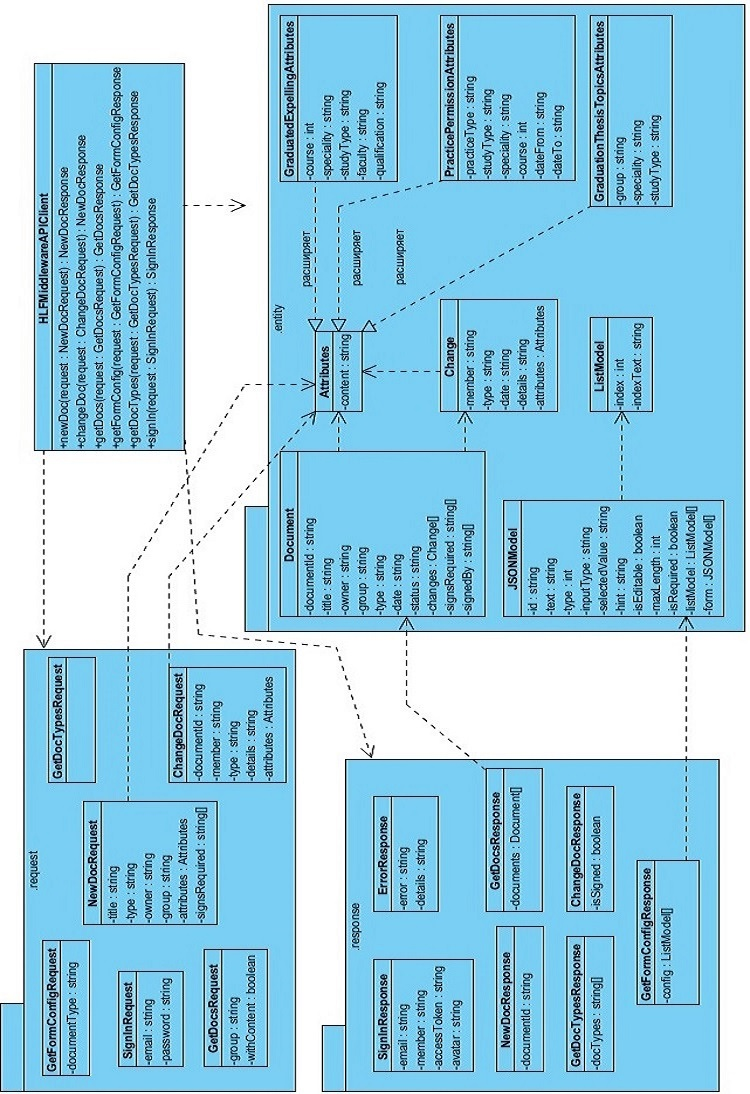
\includegraphics [scale=1.0] {MiddlewareClientNoPackageRotated}
	\caption{Диаграмма классов потребителя API связующего ПО.}
	\label{fig:MiddlewareClientNoPackage}
\end{figure}

\begin{figure}[H]
	\centering
	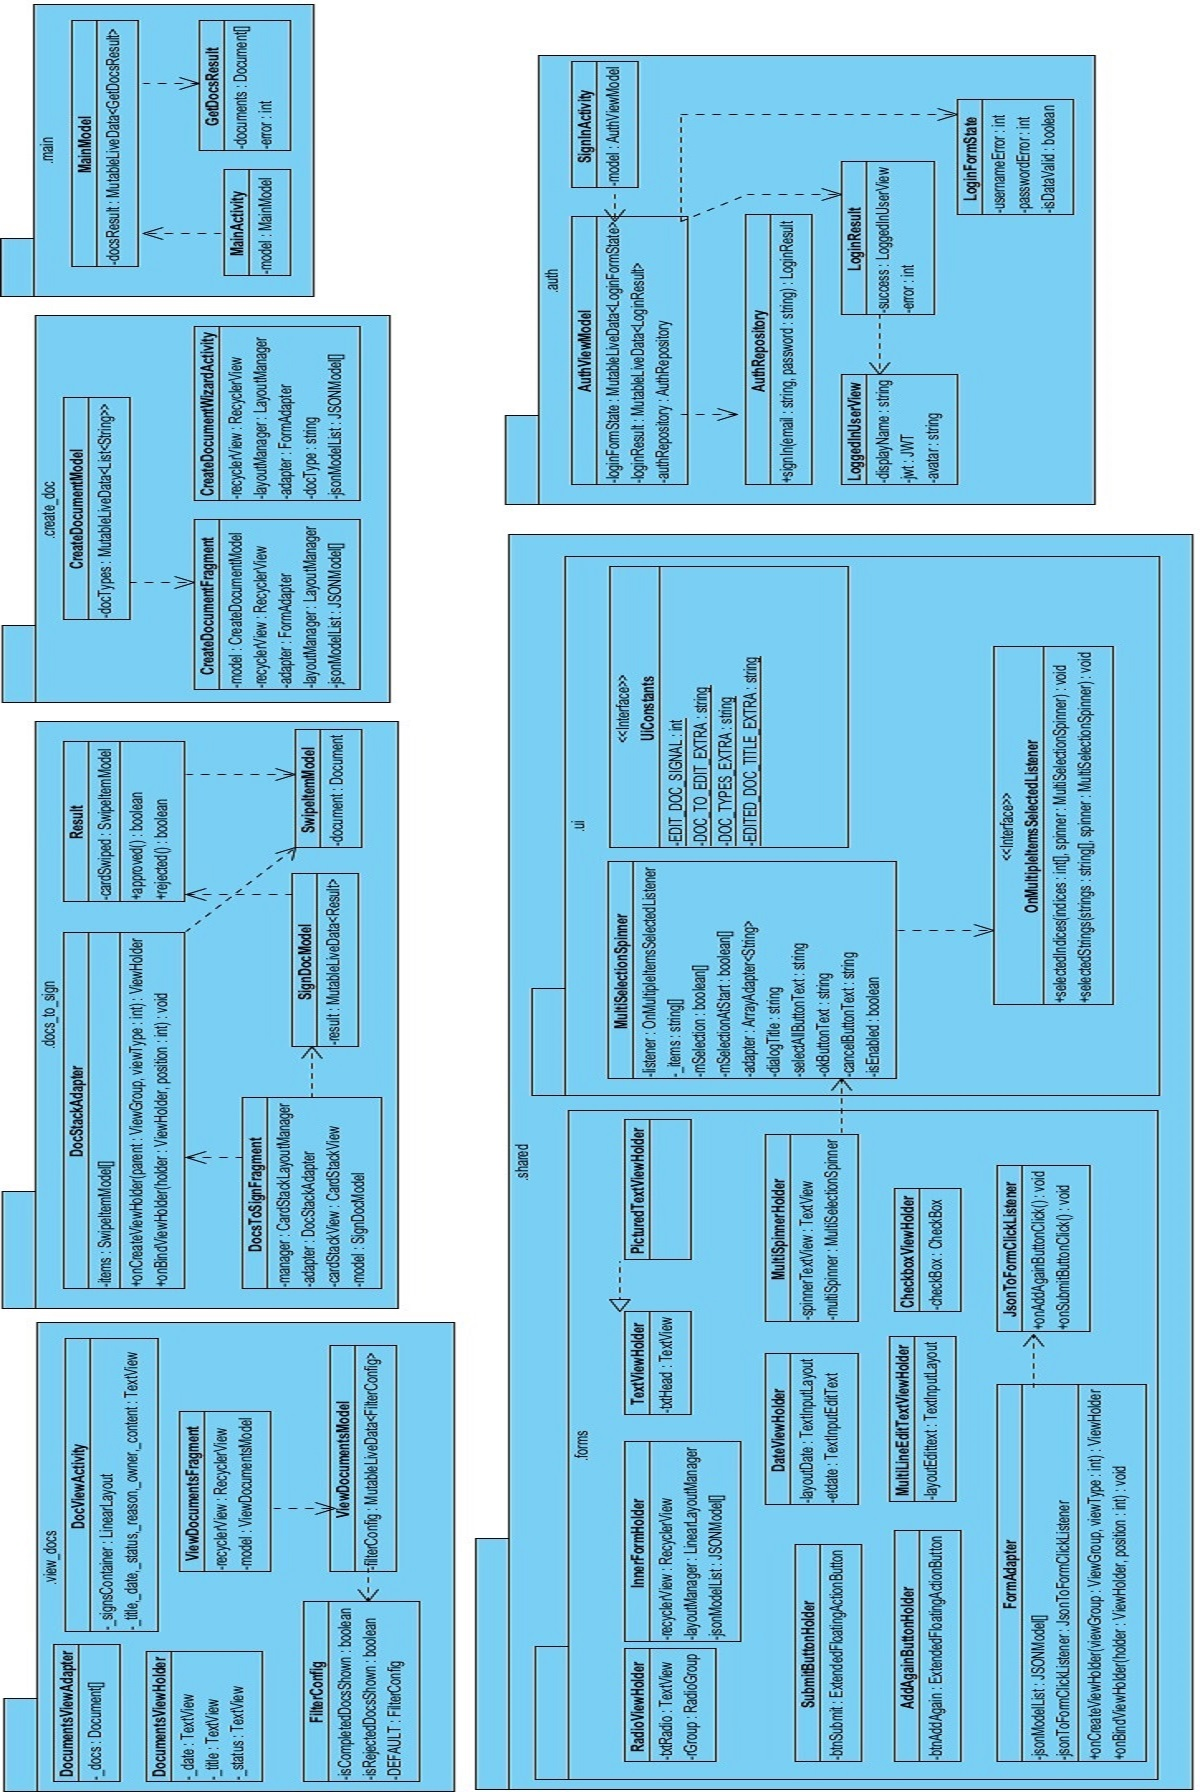
\includegraphics [scale=0.65] {UiNoPackageRotated}
	\caption{Диаграмма классов пользовательского графического интерфейса.}
	\label{fig:UiNoPackageRotated}
\end{figure}


\subsection{Пользовательский интерфейс} \label{subsec:ch3/sec2/subsec3}
Описанным в \ref{subsec:ch2/sec3/subsec4/subsubsec1} сценариям сопутствует использование графического интерфейса программы показанного на рисунках \ref{fig:ui-first} - \ref{fig:ui-last}

\begin{figure}[ht]
	\centering
	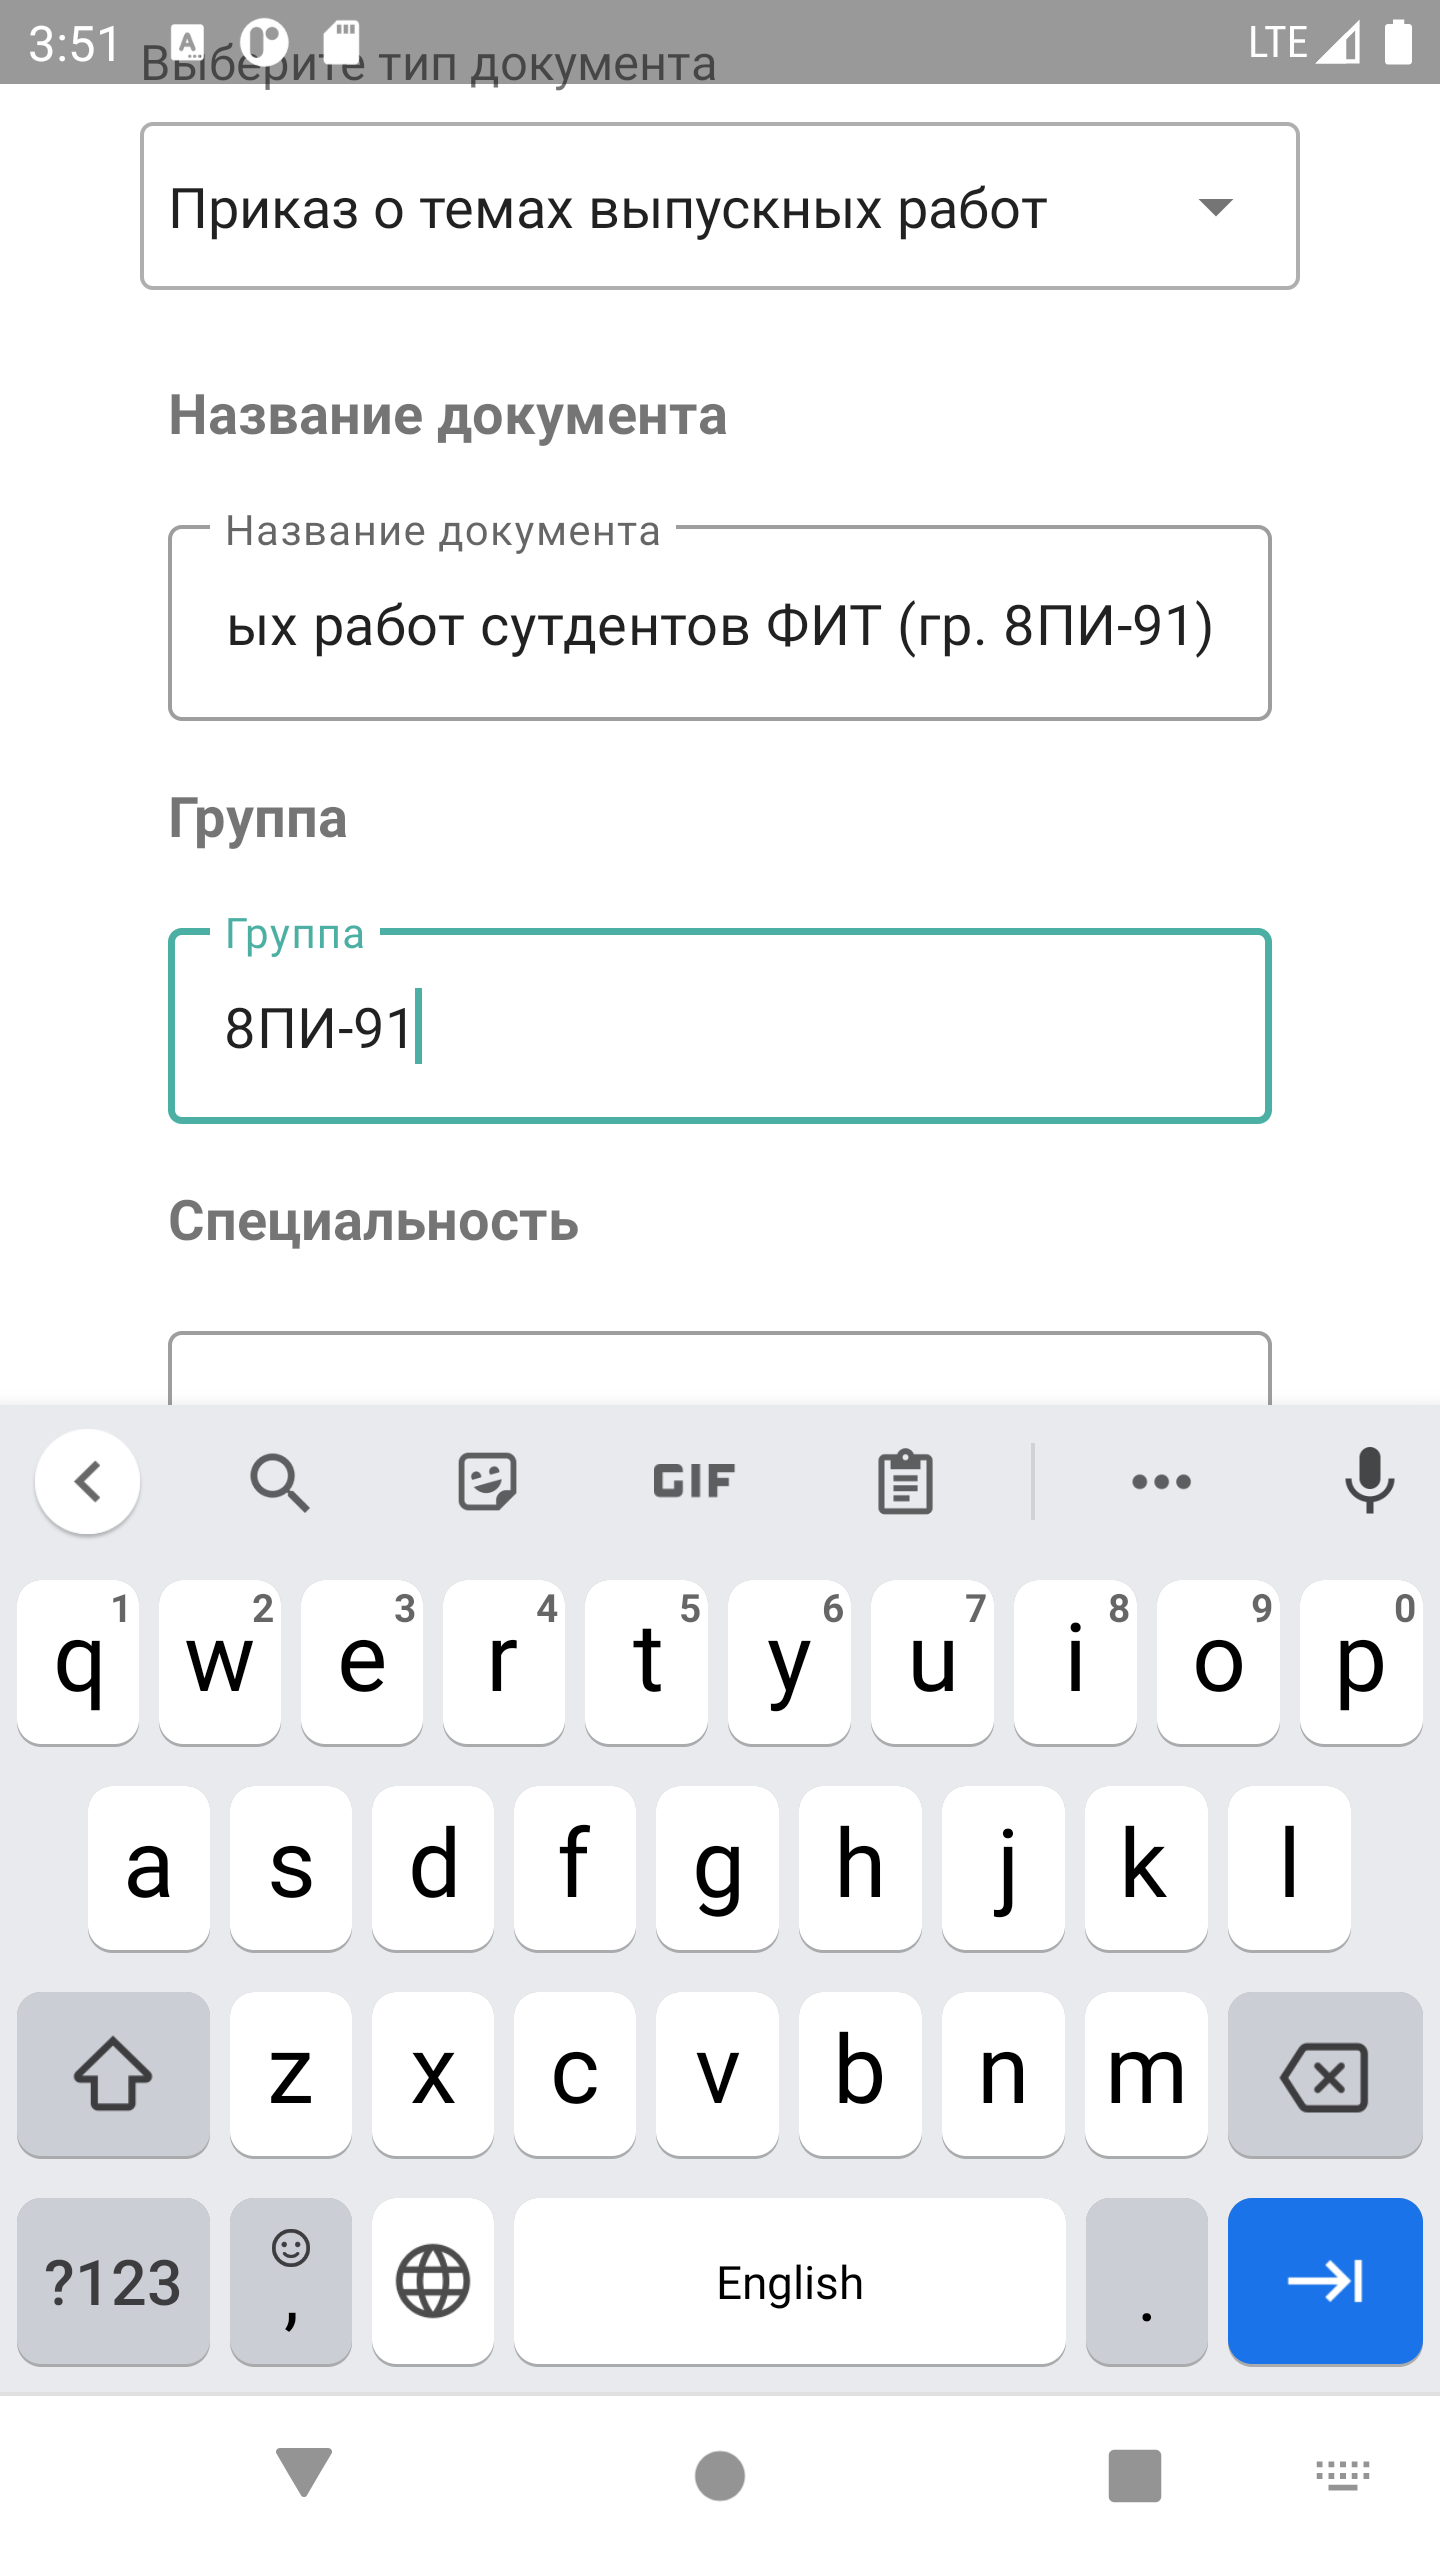
\includegraphics [scale=0.2] {doc-creating1}
	\caption{Создание документа типа "Приказ о темах выпускных работ".}
	\label{fig:ui-first}
\end{figure}

\begin{figure}[ht]
	\centering
	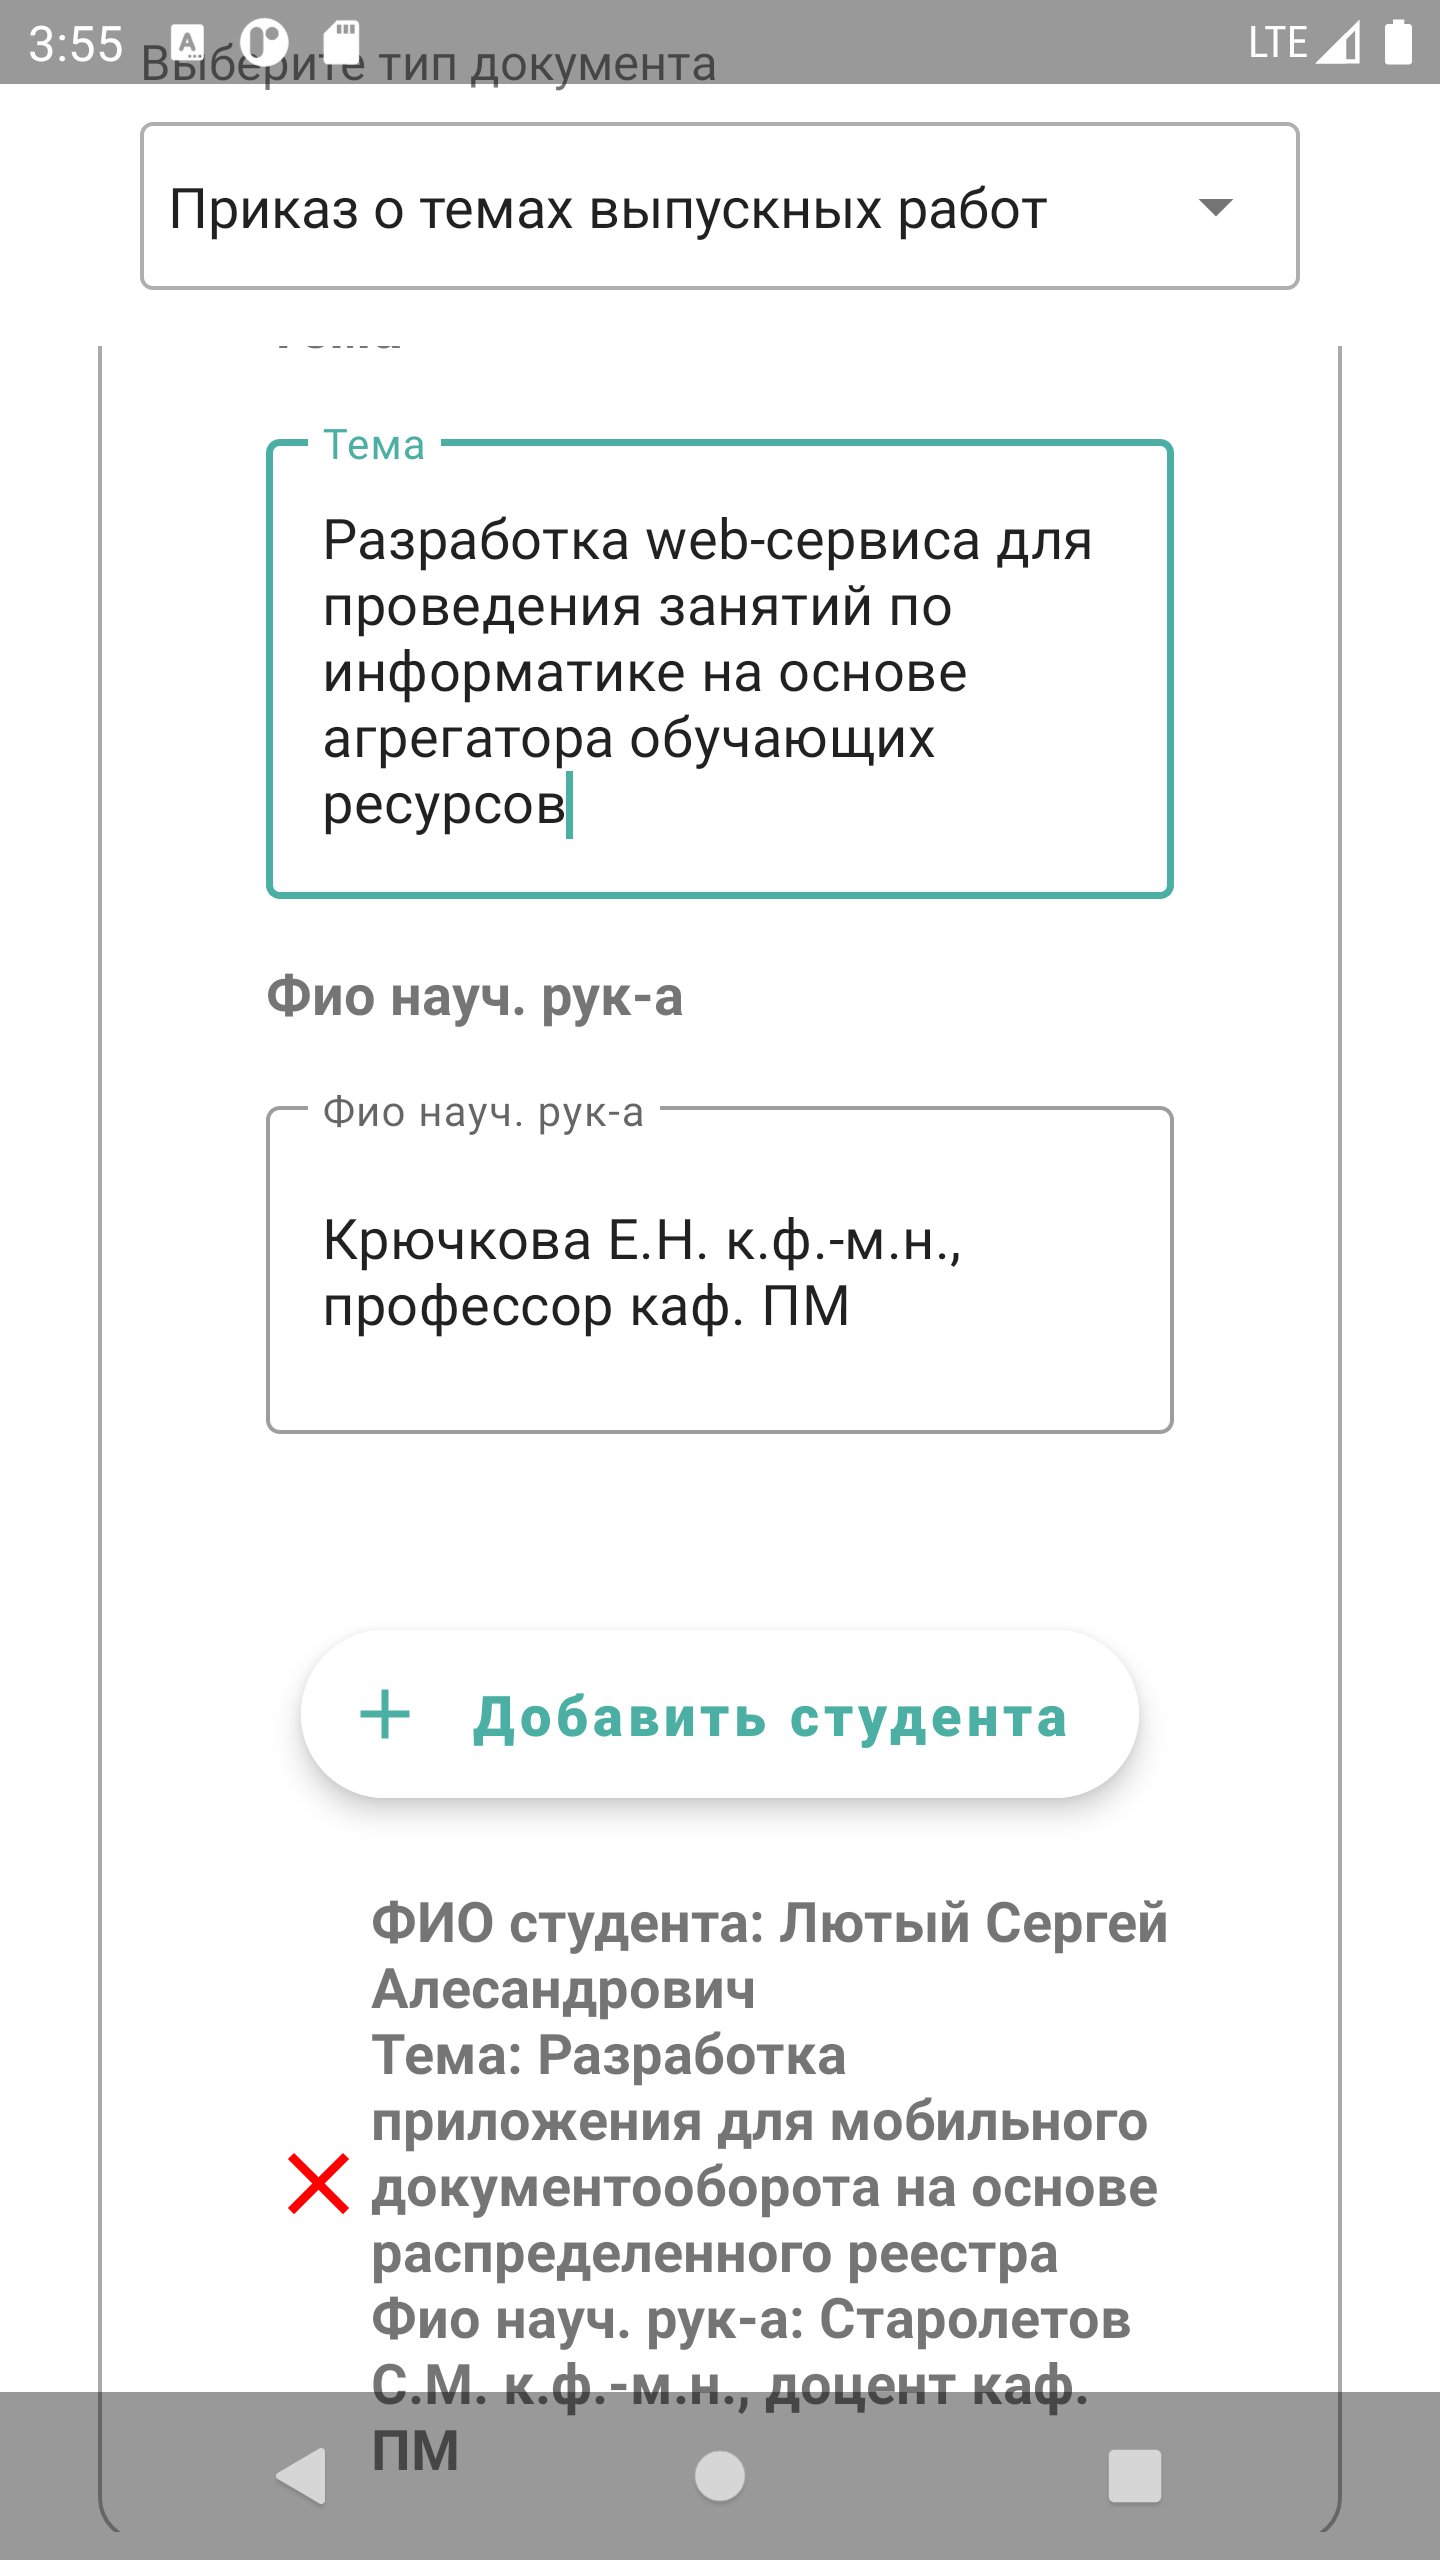
\includegraphics [scale=0.2] {doc-creating2}
	\caption{Добавление данных о студентах в создаваемый документ.}
	\label{fig:doc-creating2}
\end{figure}

\begin{figure}[ht]
	\centering
	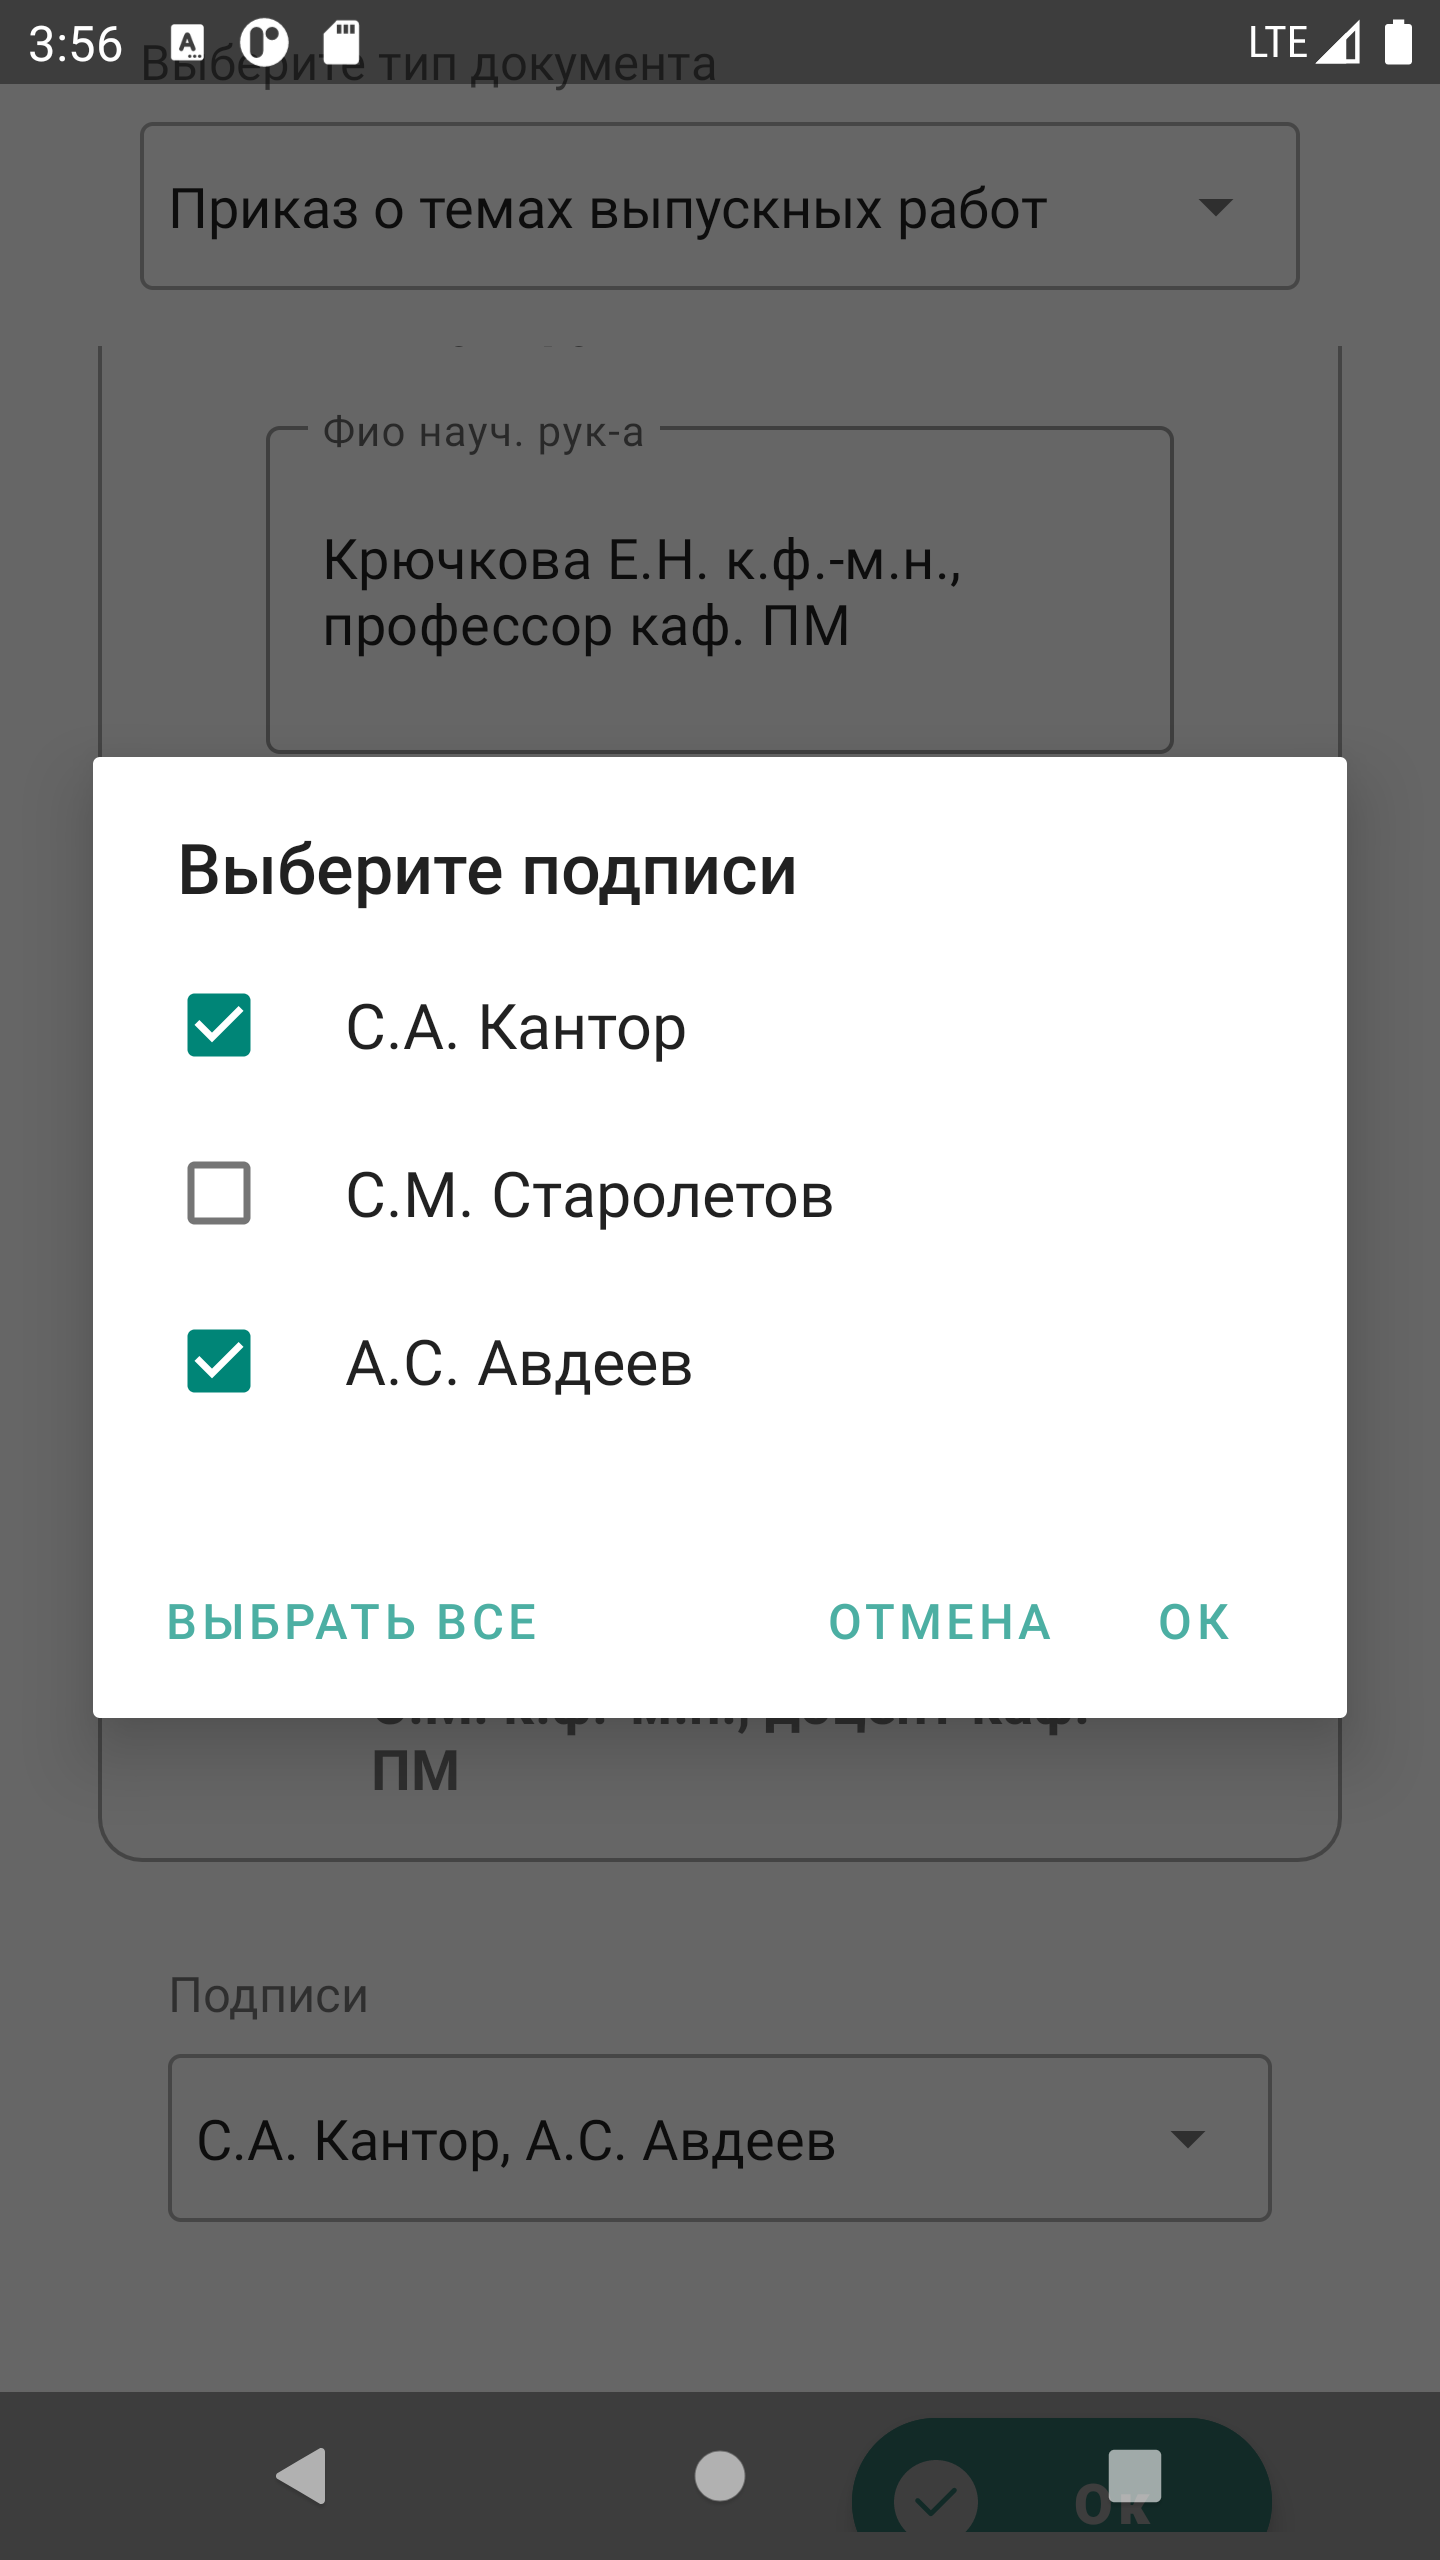
\includegraphics [scale=0.2] {doc-creating3}
	\caption{Указание необходимых подписантов.}
	\label{fig:doc-creating3}
\end{figure}

\begin{figure}[ht]
	\centering
	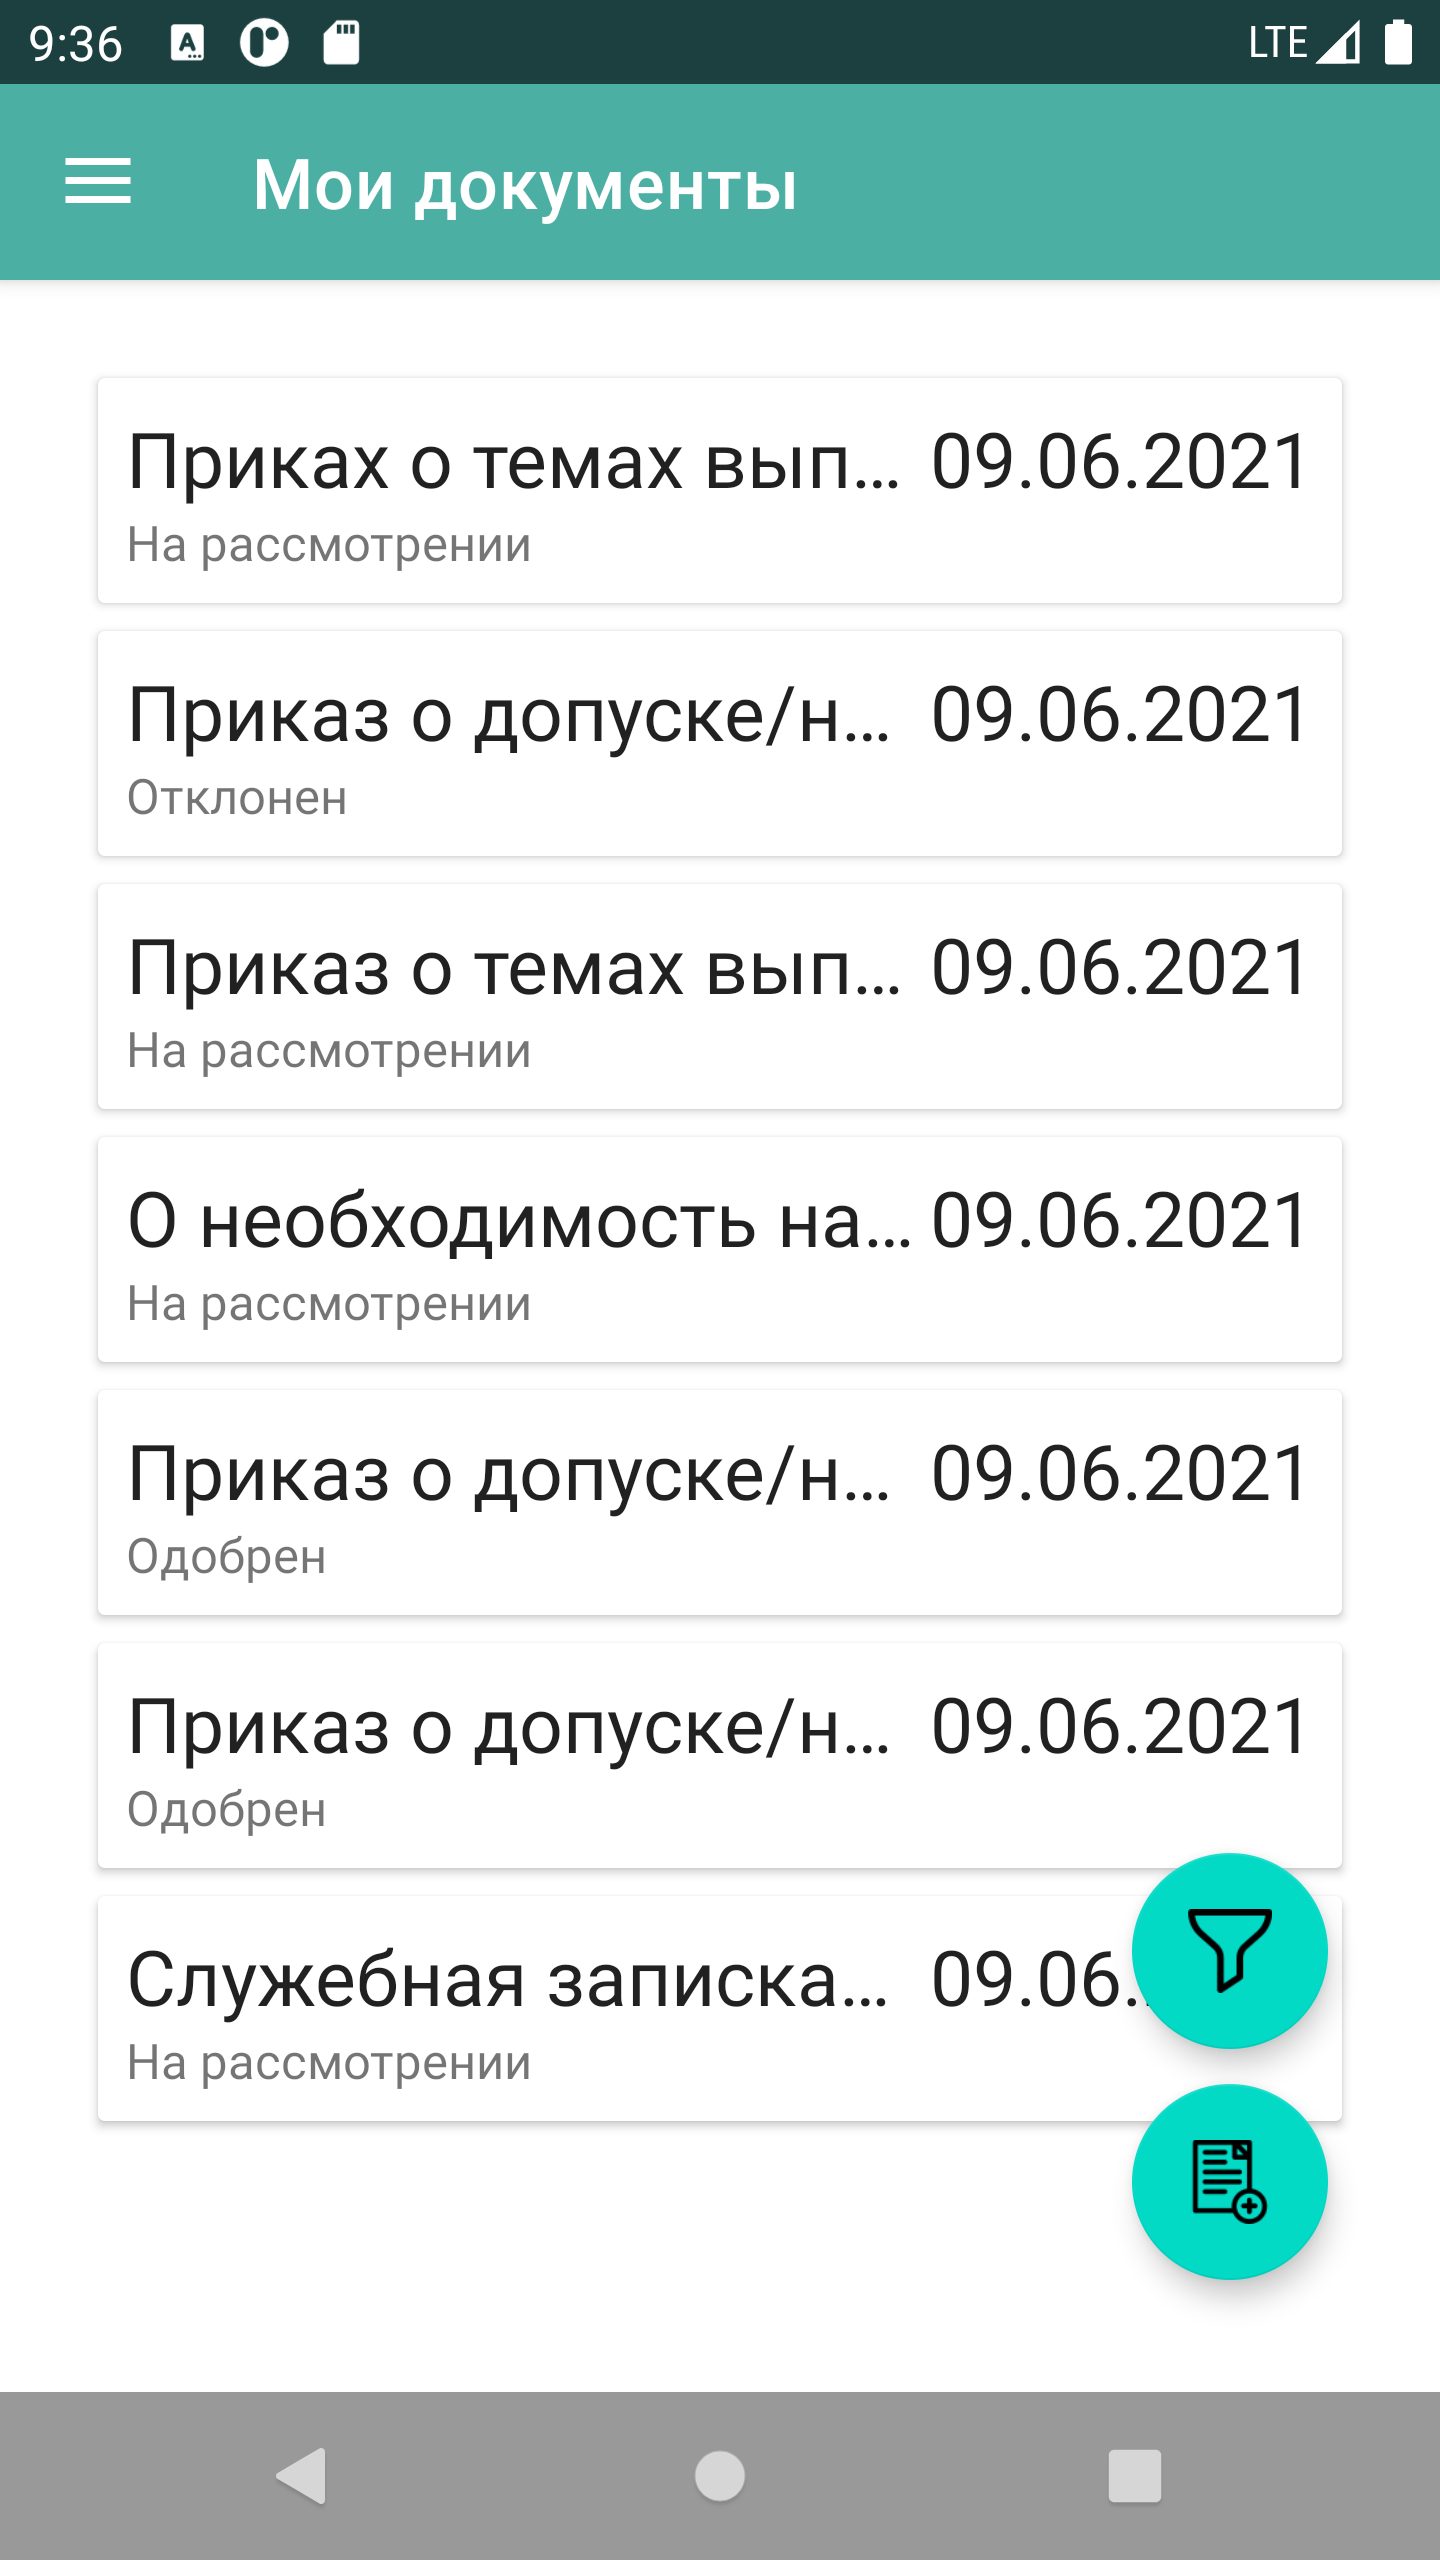
\includegraphics [scale=0.2] {before-filters}
	\caption{Список документов.}
	\label{fig:before-filters}
\end{figure}

\begin{figure}[ht]
	\centering
	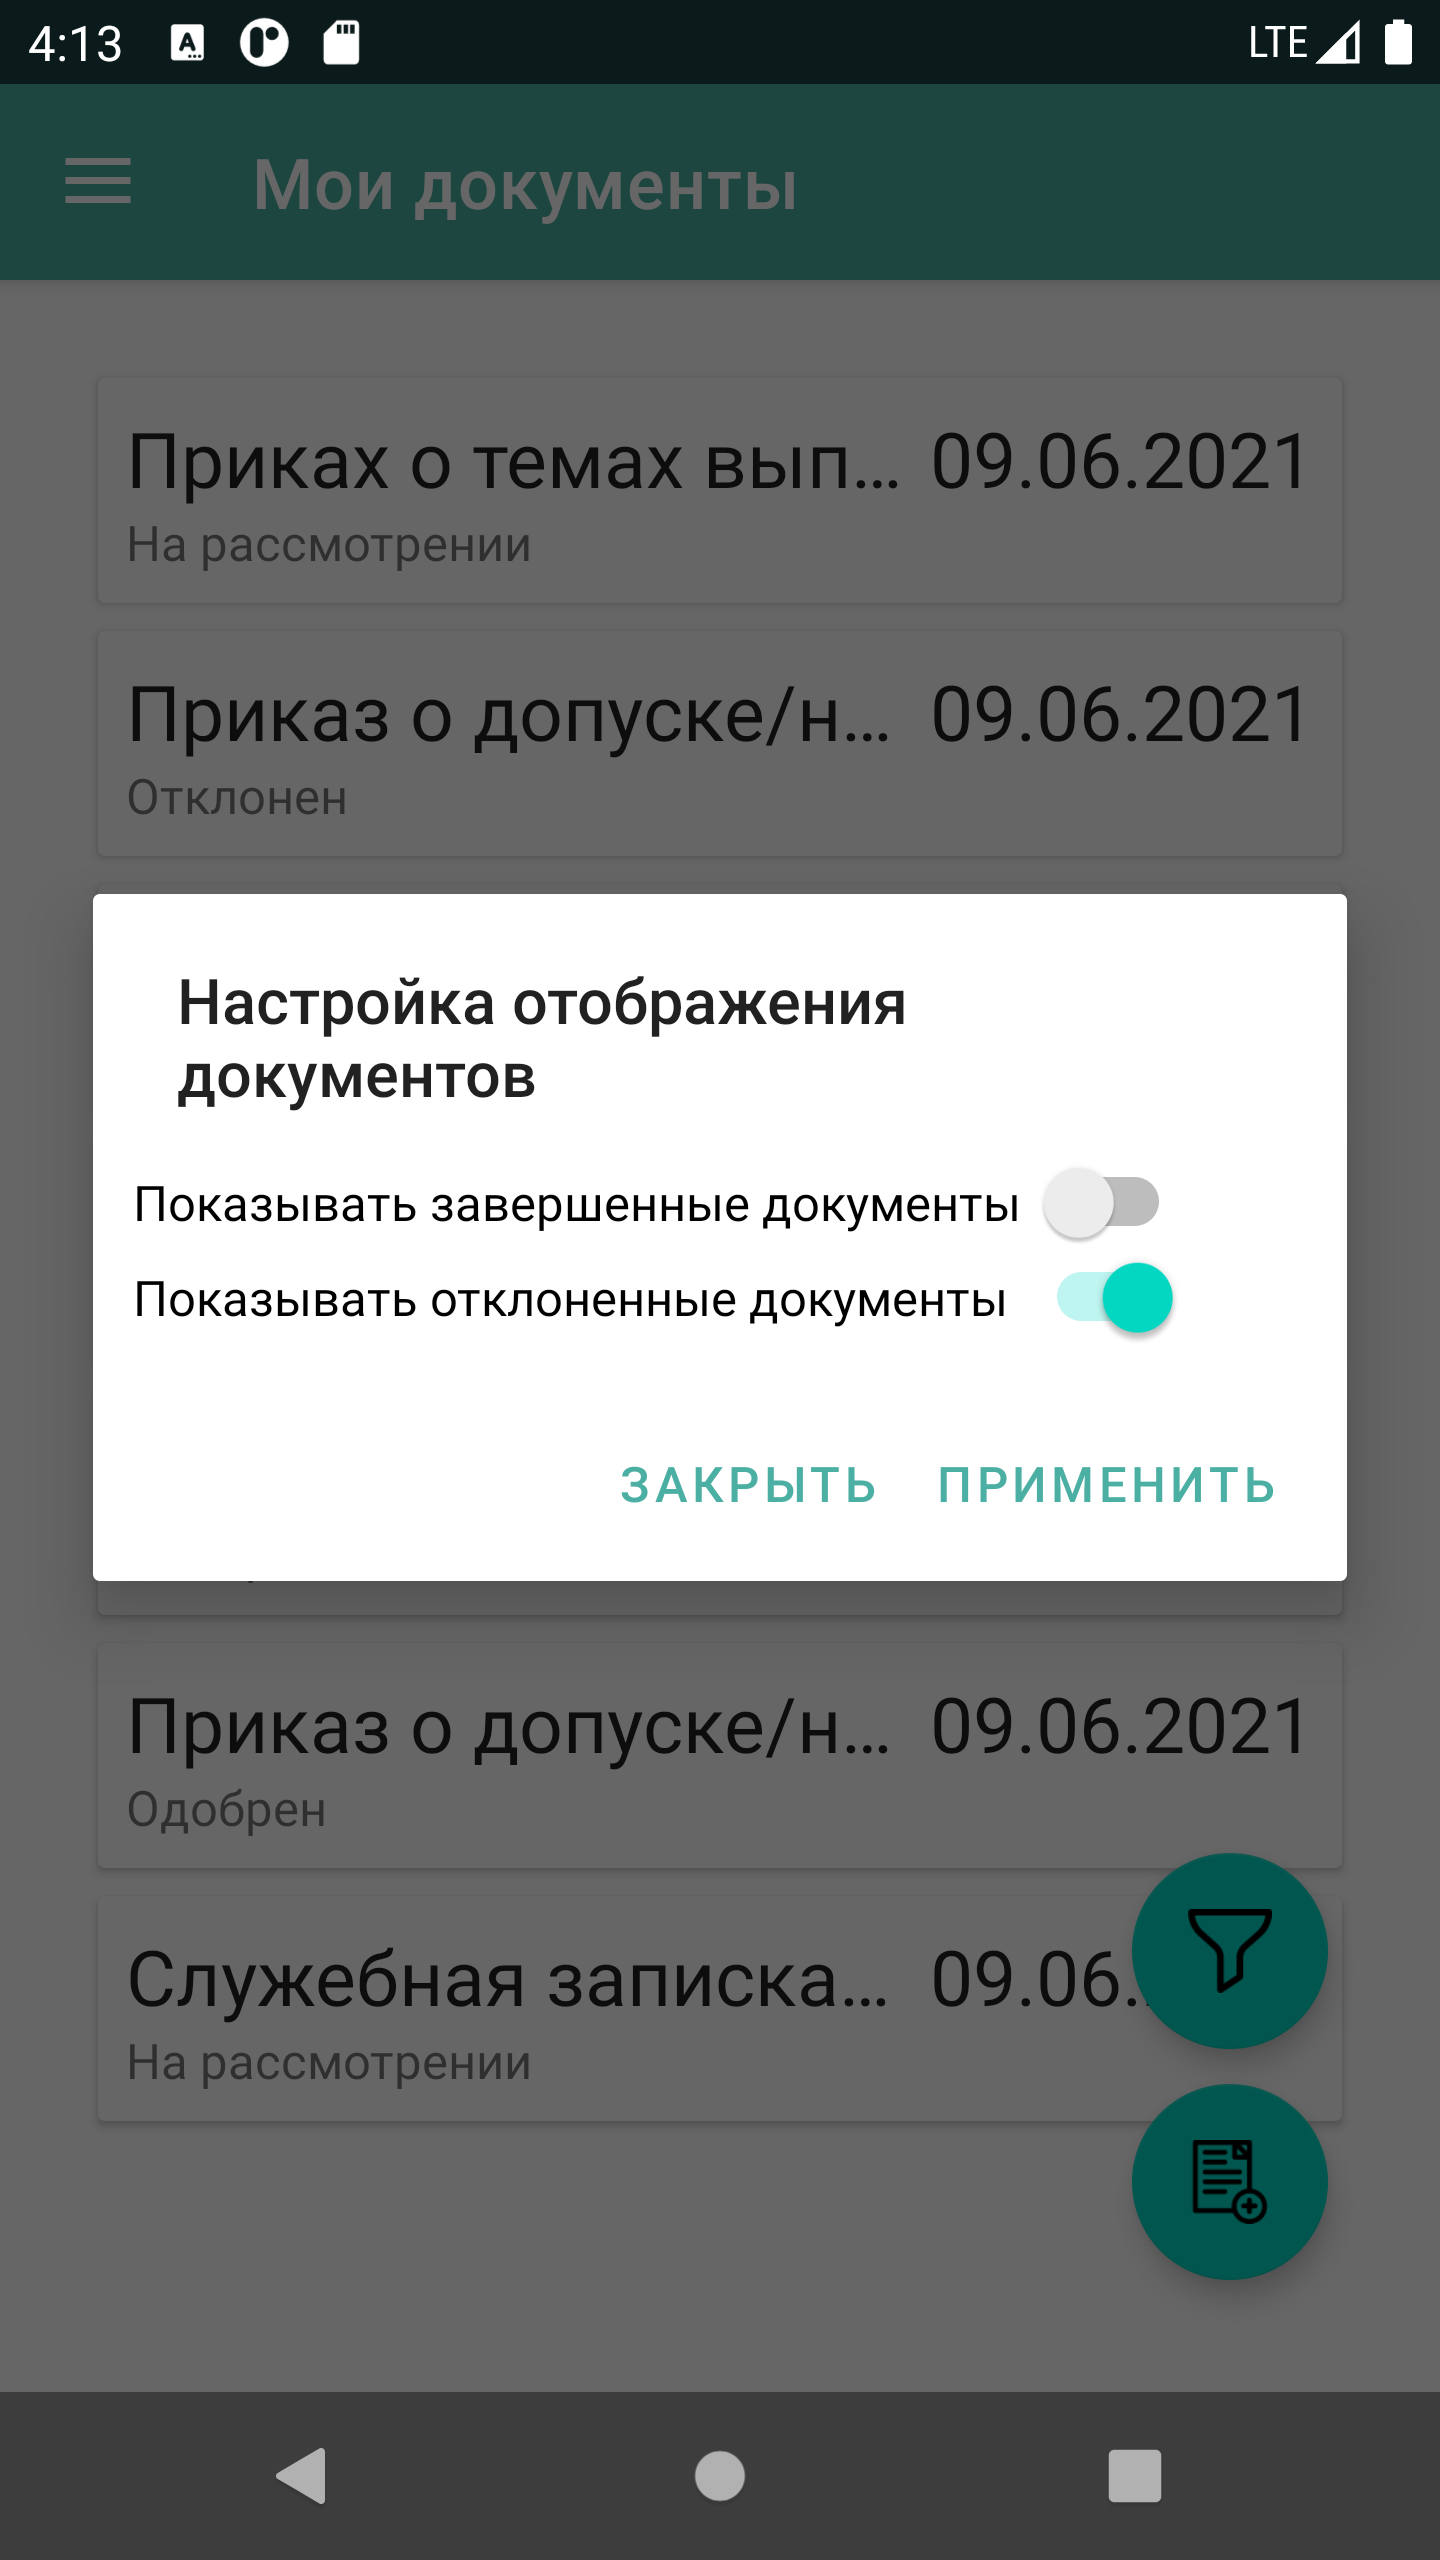
\includegraphics [scale=0.2] {filters}
	\caption{Настройка отображения списка документов.}
	\label{fig:filters}
\end{figure}

\begin{figure}[ht]
	\centering
	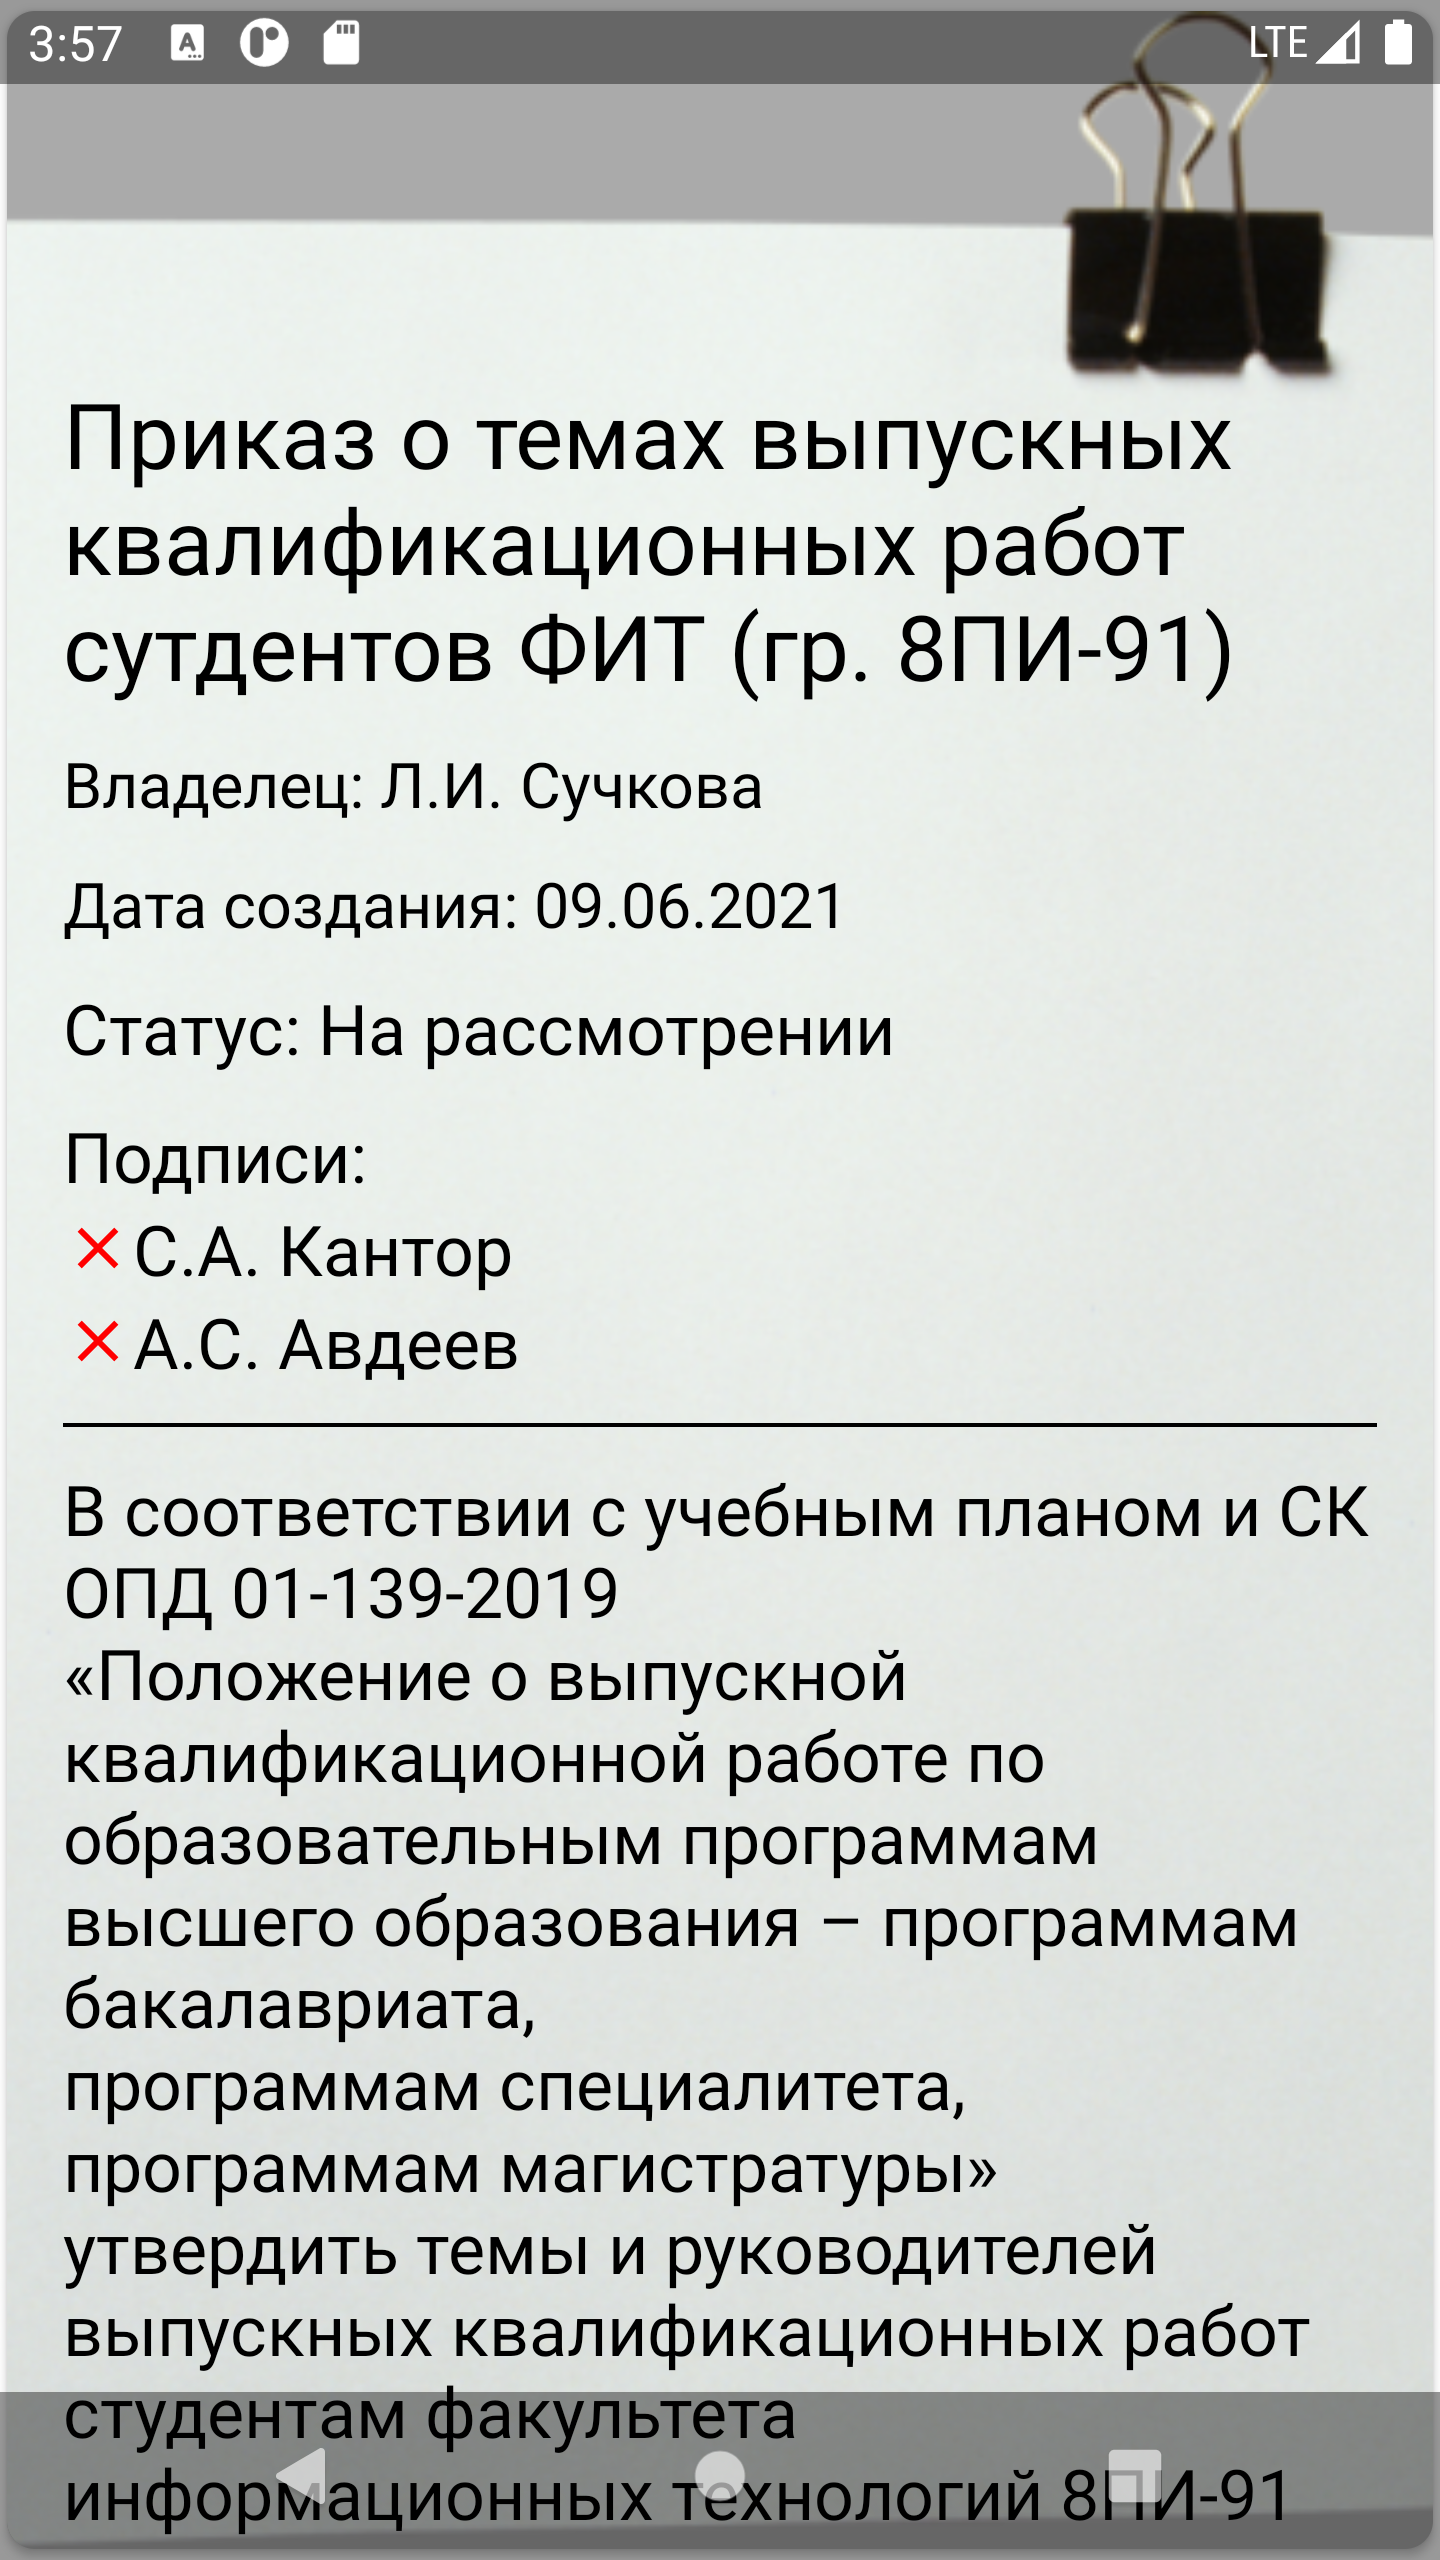
\includegraphics [scale=0.2] {doc-view}
	\caption{Просмотр деталей отдельного документа.}
	\label{fig:doc-view}
\end{figure}

\begin{figure}[ht]
	\centering
	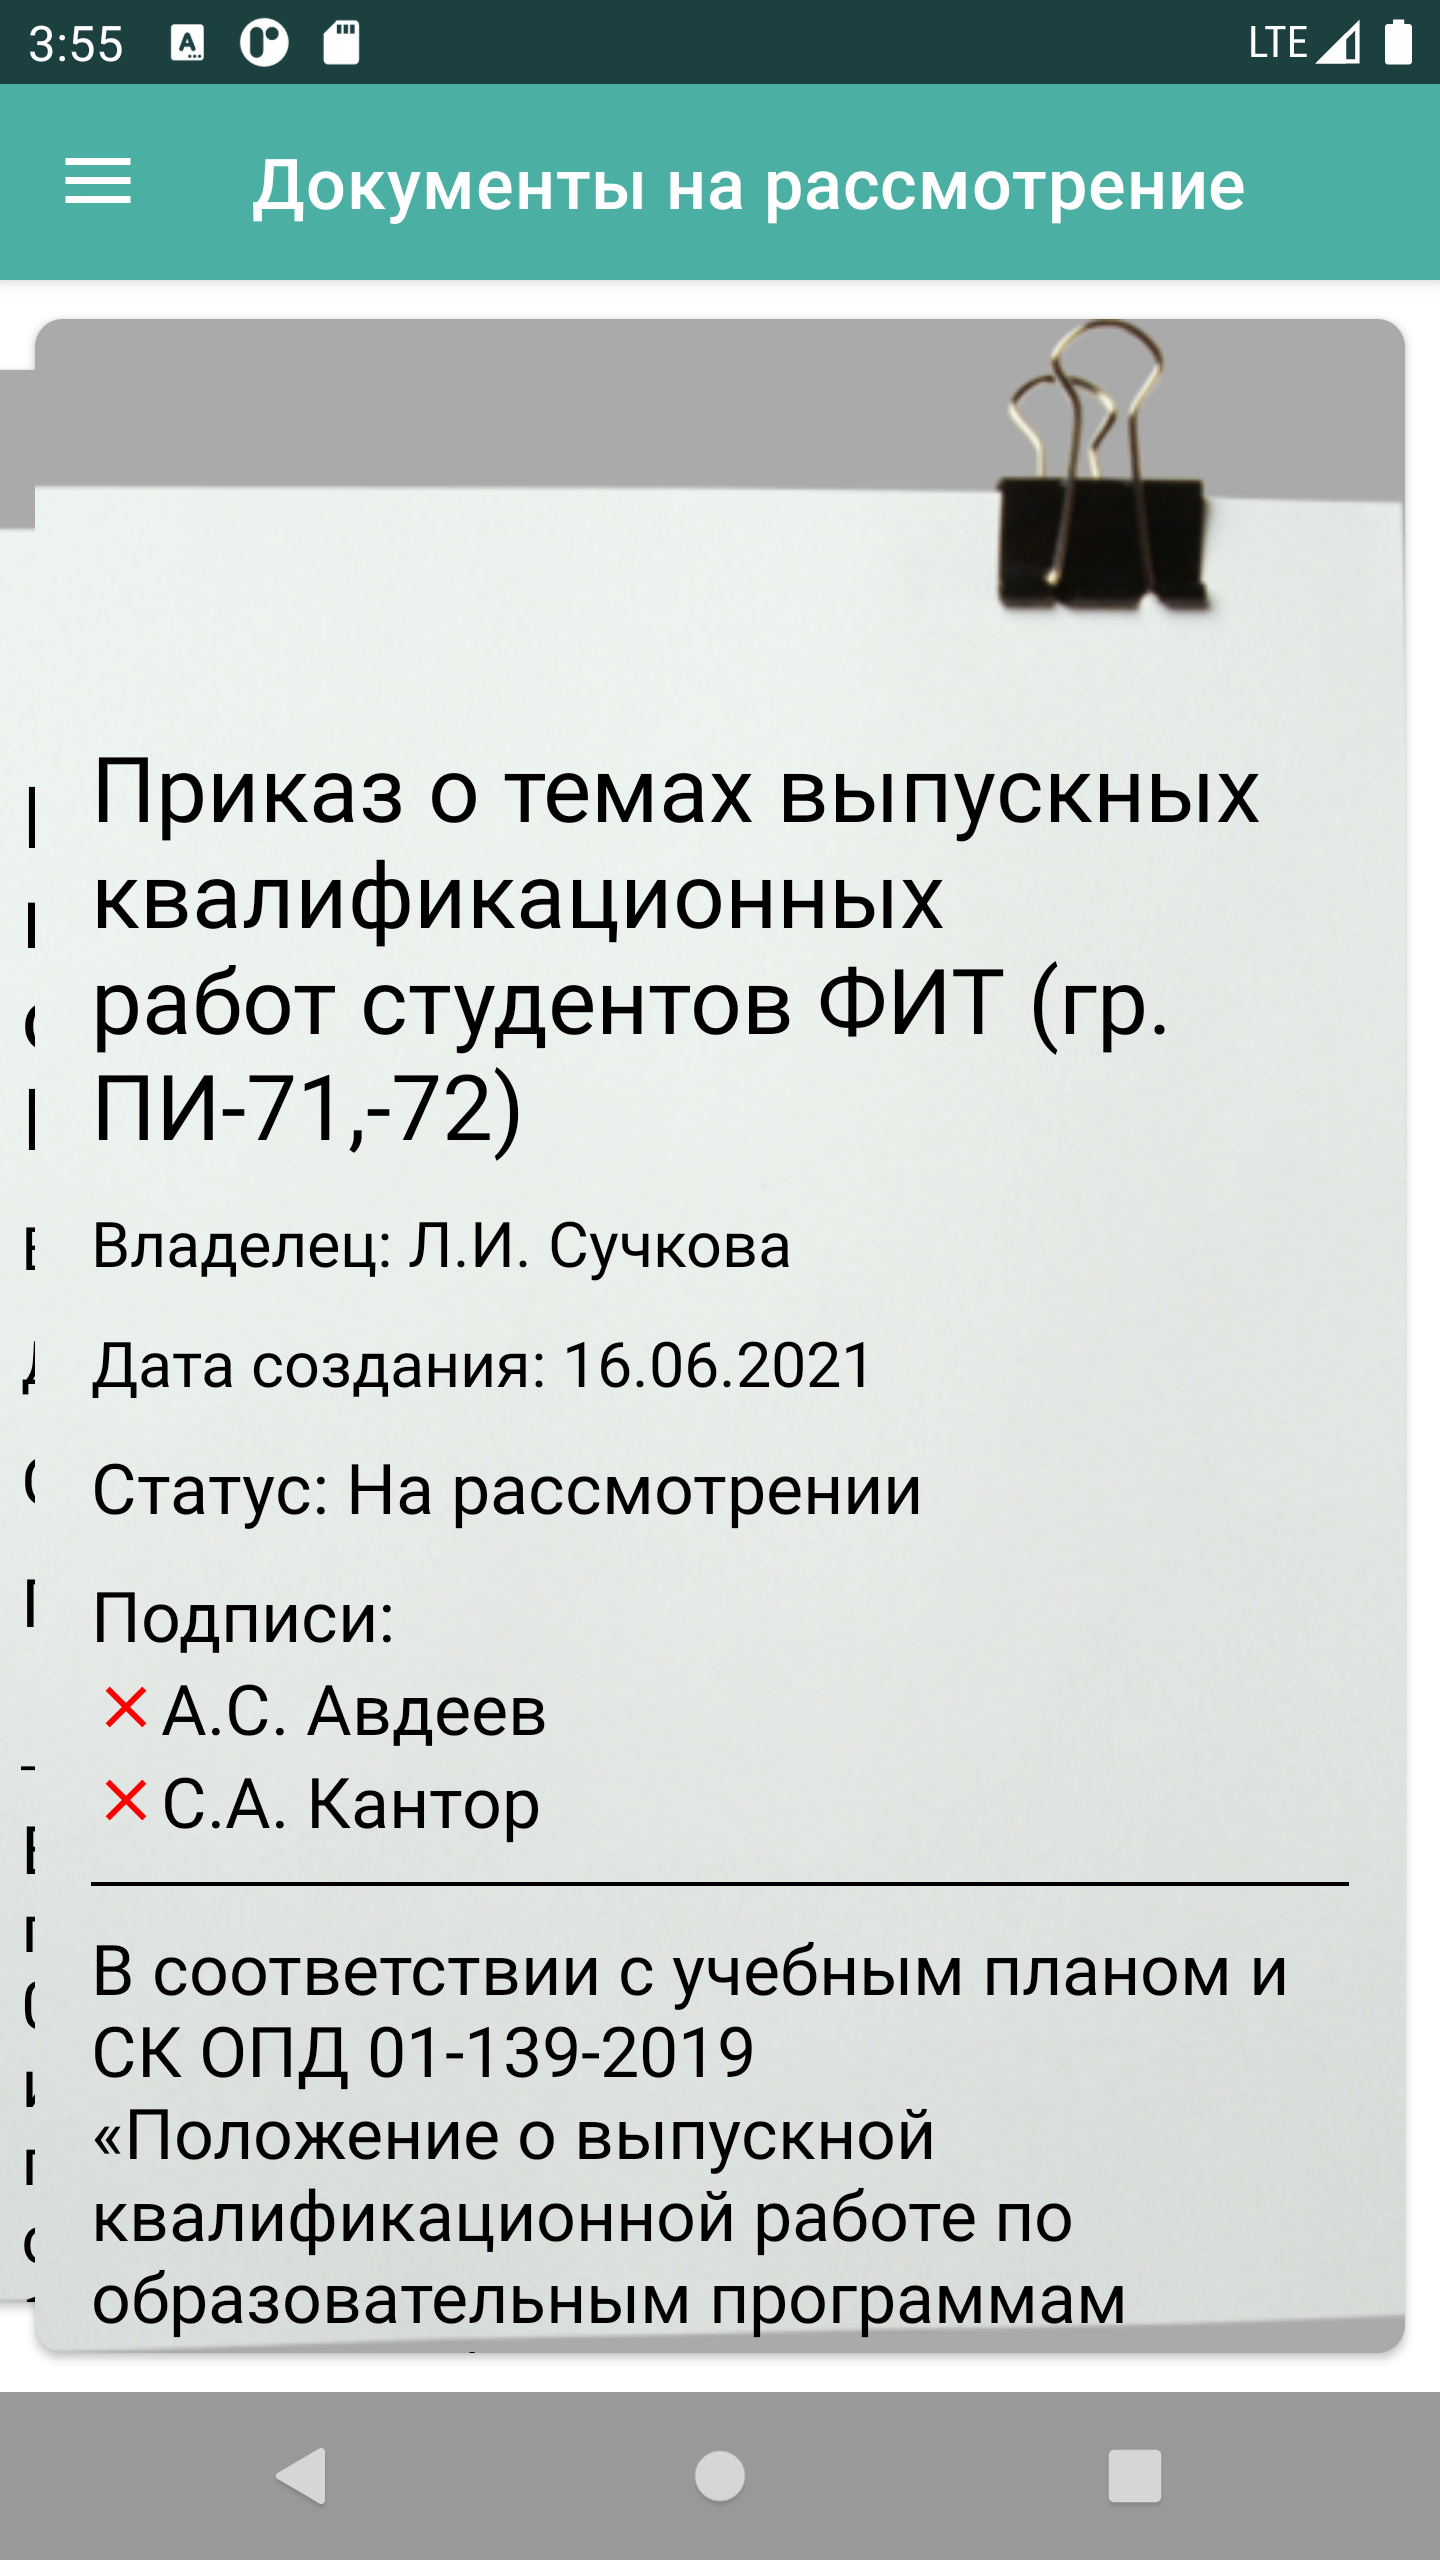
\includegraphics [scale=0.2] {doc-stack}
	\caption{Стопка документов на рассмотрение.}
	\label{fig:doc-stack}
\end{figure}

\begin{figure}[ht]
	\centering
	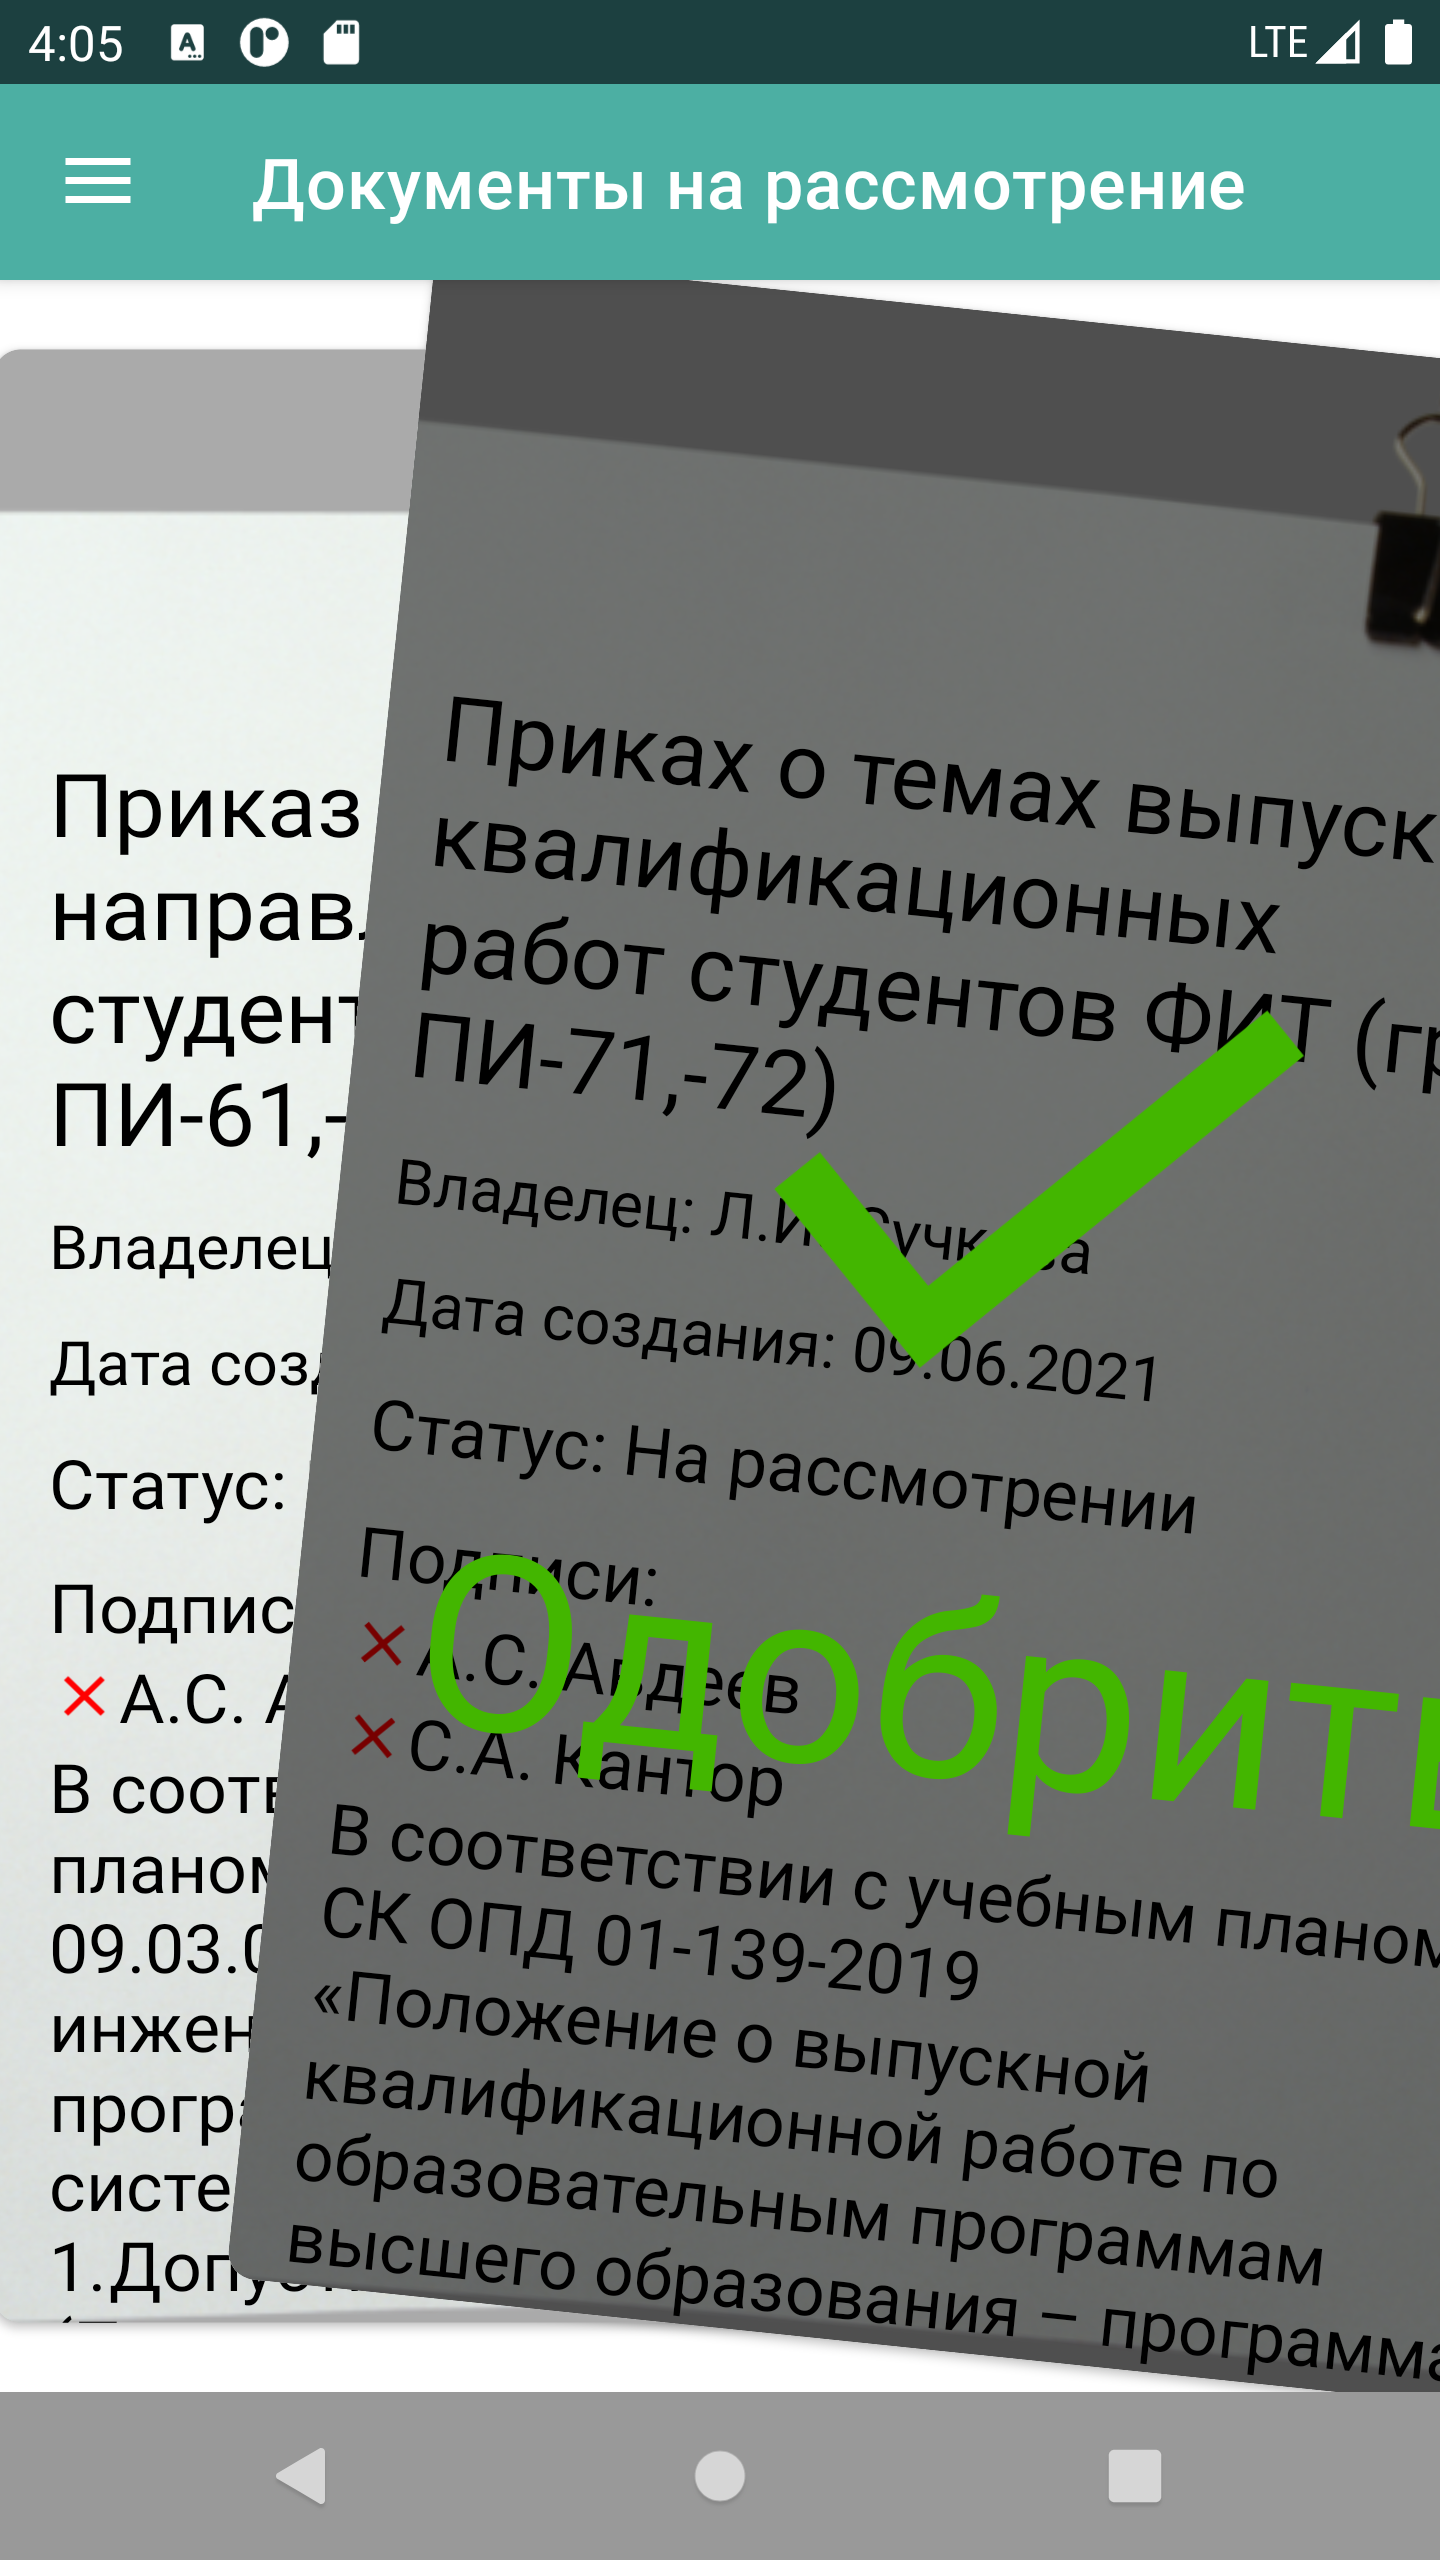
\includegraphics [scale=0.2] {approve}
	\caption{Одобрение (подписывание) документа.}
	\label{fig:approve}
\end{figure}

\begin{figure}[ht]
	\centering
	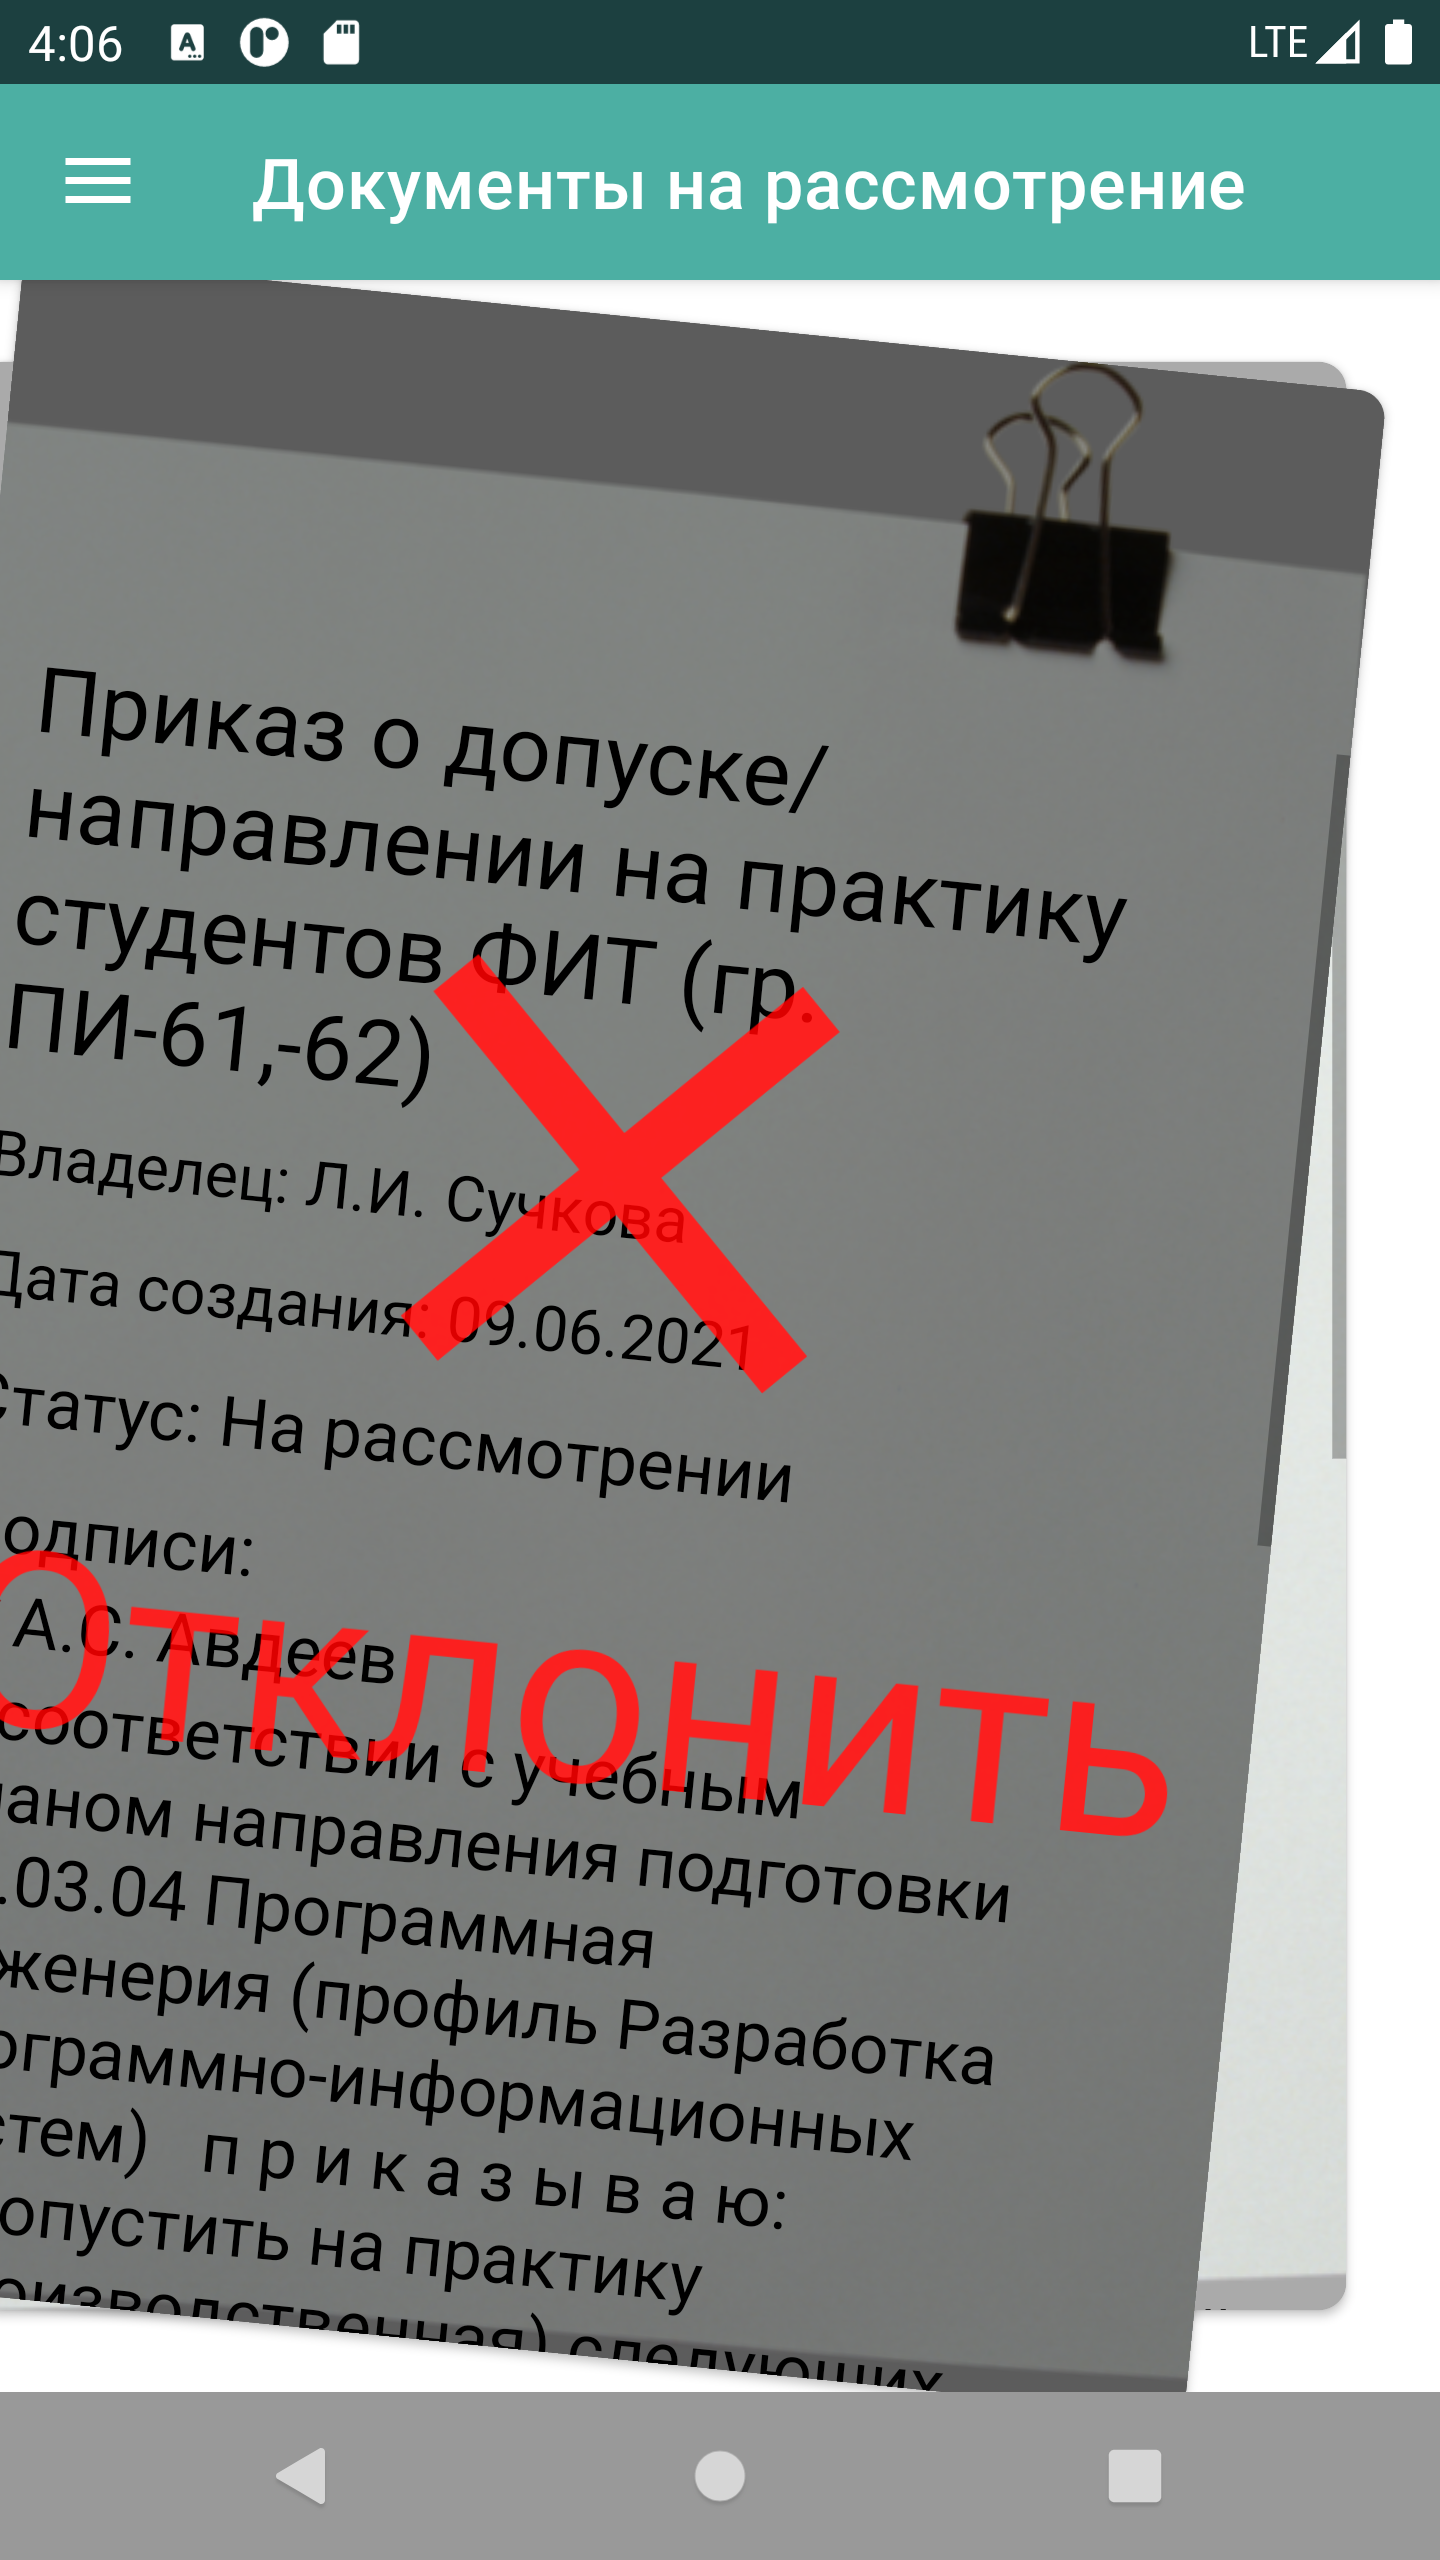
\includegraphics [scale=0.2] {reject}
	\caption{Отклонение документа.}
	\label{fig:reject}
\end{figure}

\begin{figure}[ht]
	\centering
	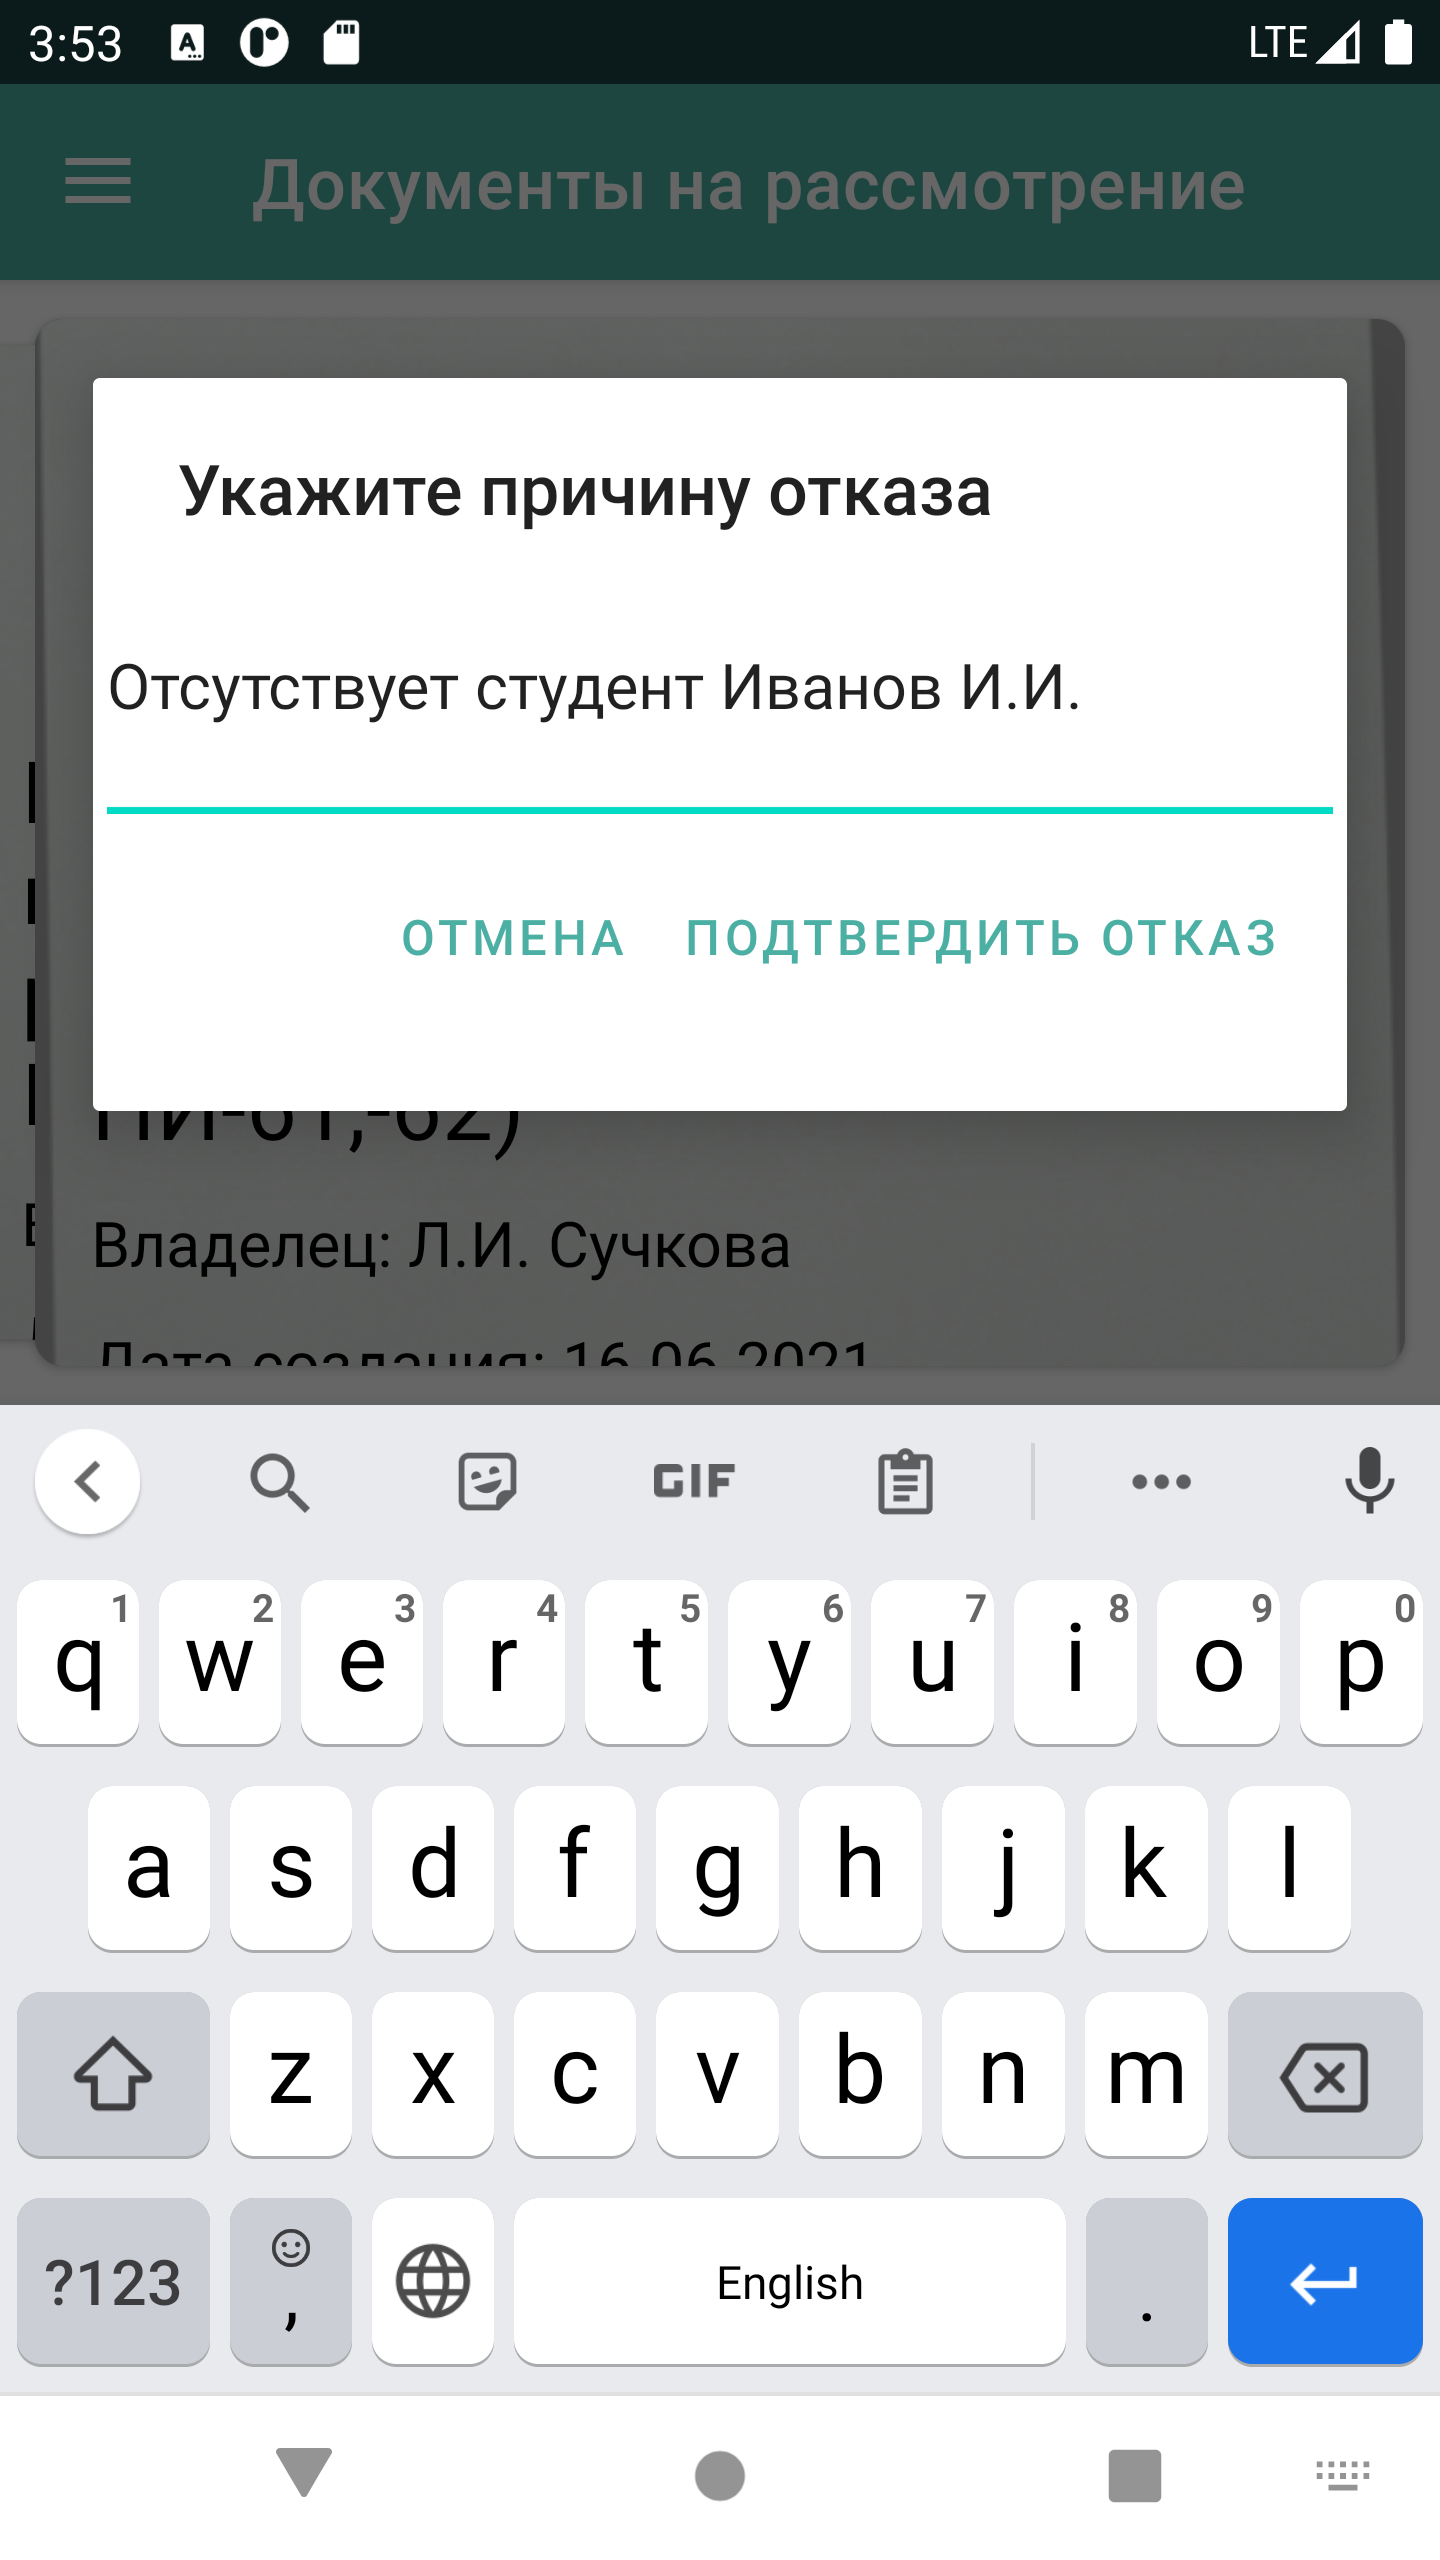
\includegraphics [scale=0.2] {reason-for-reject}
	\caption{Указание причины отказа в качестве комментария.}
	\label{fig:ui-last}
\end{figure}           % <== Глава 3
\chapter*{\centerline{Заключение}}                     % Заголовок
\addcontentsline{toc}{chapter}{Заключение}  % Добавляем его в оглавление

%% Согласно ГОСТ Р 7.0.11-2011:
%% 5.3.3 В заключении диссертации излагают итоги выполненного исследования, рекомендации, перспективы дальнейшей разработки темы.
%% 9.2.3 В заключении автореферата диссертации излагают итоги данного исследования, рекомендации и перспективы дальнейшей разработки темы.
%% Поэтому имеет смысл сделать эту часть общей и загрузить из одного файла в автореферат и в диссертацию:

В процессе работы был реализован децентрализованный мобильный документооборот для вуза. Разработанная система отвечает всем функциональным требованиям, которые были к ней выдвинуты. 

А именно: она позволят создавать и хранить в блокчейне как общие, так и специфические для некоторого типа атрибуты документов. К общим можно отнести название, текст документа и список подписантов, участвующих в жизненном цикле документа. А к специфическим можно отнести факультет, группу и т.д. в случае приказа об отчислении в связи окончанием обучения. Также система позволяет пользователям просматривать список документов в рассмотрении которых они участвуют. Функционал мобильного приложения позволяет настроить отображение списка документов. Такие операции как редактирование, подписание, отклонение, комментирование выполняются пользователями в мобильном приложении с задействованием интерактивности мобильной платформы, а именно инициация данных действий осуществляется "смахиванием" документа с представленной пользователю стопки документа. В системе достигнута возможность легкого расширения диапазона шаблонных документов, путем не требующих особых усилий действий разработчика. 
Так же обеспечена последовательность подписи - пользователь, очередь которого одобрить или отклонить по какой либо причине еще не подошла не имеет физической возможности этого сделать. Он может только отслеживать изменение его состояния. Кроме того в разработанном СЭД достигнут достаточный уровень безопасности, за счет того что он основан на технологии блокчейн. Это максимально затрудняет нежелательно изменение состояния хранимых документов.


Тезисы работы были представлены на конференции "Наука и молодежь 2021" в секции "Информационные технологии".
      % <== Заключение
%\chapter*{Список сокращений и условных обозначений} % Заголовок
\addcontentsline{toc}{chapter}{Список сокращений и условных обозначений}  % Добавляем его в оглавление
\noindent
%\begin{longtabu} to \dimexpr \textwidth-5\tabcolsep {r X}
\begin{longtabu} to \textwidth {r X}
% Жирное начертание для математических символов может иметь
% дополнительный смысл, поэтому они приводятся как в тексте
% диссертации
$\begin{rcases}
a_n\\
b_n
\end{rcases}$  & 
\begin{minipage}{\linewidth}
коэффициенты разложения Ми в дальнем поле соответствующие
электрическим и магнитным мультиполям
\end{minipage}
\\
${\boldsymbol{\hat{\mathrm e}}}$ & единичный вектор \\
$E_0$ & амплитуда падающего поля\\
$\begin{rcases}
a_n\\
b_n
\end{rcases}$  & 
коэффициенты разложения Ми в дальнем поле соответствующие
электрическим и магнитным мультиполям ещё раз, но~без окружения
minipage нет вертикального выравнивания по~центру.
\\
$j$ & тип функции Бесселя\\
$k$ & волновой вектор падающей волны\\

$\begin{rcases}
a_n\\
b_n
\end{rcases}$  & 
\begin{minipage}{\linewidth}
\vspace{0.7em}
и снова коэффициенты разложения Ми в дальнем поле соответствующие
электрическим и магнитным мультиполям, теперь окружение minipage есть
и добавлено много текста, так что описание группы условных
обозначений значительно превысило высоту этой группы... Для отбивки
пришлось добавить дополнительные отступы.
\vspace{0.5em}
\end{minipage}
\\
$L$ & общее число слоёв\\
$l$ & номер слоя внутри стратифицированной сферы\\
$\lambda$ & длина волны электромагнитного излучения
в вакууме\\
$n$ & порядок мультиполя\\
$\begin{rcases}
{\mathbf{N}}_{e1n}^{(j)}&{\mathbf{N}}_{o1n}^{(j)}\\
{\mathbf{M}_{o1n}^{(j)}}&{\mathbf{M}_{e1n}^{(j)}}
\end{rcases}$  & сферические векторные гармоники\\
$\mu$  & магнитная проницаемость в вакууме\\
$r,\theta,\phi$ & полярные координаты\\
$\omega$ & частота падающей волны\\

\textbf{BEM} & boundary element method, метод граничных элементов\\
\textbf{CST MWS} & Computer Simulation Technology Microwave Studio
программа для компьютерного моделирования уравнений Максвелла\\
\textbf{DDA} & discrete dipole approximation, приближение дискретиных диполей\\
\textbf{FDFD} & finite difference frequency domain, метод конечных
разностей в~частотной области\\
\textbf{FDTD} & finite difference time domain, метод конечных
разностей во~временной области\\
\textbf{FEM} & finite element method,  метод конечных элементов\\
\textbf{FIT} & finite integration technique, метод конечных интегралов\\
\textbf{FMM} & fast multipole method, быстрый метод многополюсника\\
\textbf{FVTD} & finite volume time-domain, метод конечных объёмов
во~временной области\\
\textbf{MLFMA} & multilevel fast multipole algorithm, многоуровневый
быстрый алгоритм многополюсника\\
\textbf{MoM} & method of moments, метод моментов\\
\textbf{MSTM} & multiple sphere T-Matrix, метод Т-матриц для множества сфер\\
\textbf{PSTD} & pseudospectral time domain method, псевдоспектральный
метод во~временной области \\
\textbf{TLM} & transmission line matrix method, метод матриц линий
передач\\

\end{longtabu}
\addtocounter{table}{-1}% Нужно откатить на единицу счетчик номеров таблиц, так как предыдующая таблица сделана для удобства представления информации по ГОСТ
        % Список сокращений и условных обозначений
%\chapter*{Словарь терминов}             % Заголовок
\addcontentsline{toc}{chapter}{Словарь терминов}  % Добавляем его в оглавление

\textbf{TeX} : Cистема компьютерной вёрстки, разработанная американским профессором информатики Дональдом Кнутом

\textbf{панграмма} : Короткий текст, использующий все или почти все буквы алфавита
      % Словарь терминов
\clearpage                                  % В том числе гарантирует, что список литературы в оглавлении будет с правильным номером страницы
%\hypersetup{ urlcolor=black }               % Ссылки делаем чёрными
%\providecommand*{\BibDash}{}                % В стилях ugost2008 отключаем использование тире как разделителя
\urlstyle{rm}                               % ссылки URL обычным шрифтом
\ifdefmacro{\microtypesetup}{\microtypesetup{protrusion=false}}{} % не рекомендуется применять пакет микротипографики к автоматически генерируемому списку литературы
\insertbibliofull                           % Подключаем Bib-базы
\ifdefmacro{\microtypesetup}{\microtypesetup{protrusion=true}}{}
\urlstyle{tt}                               % возвращаем установки шрифта ссылок URL
%\hypersetup{ urlcolor={urlcolor} }          % Восстанавливаем цвет ссылок      % <== Список литературы 
%\clearpage
\ifdefmacro{\microtypesetup}{\microtypesetup{protrusion=false}}{} % не рекомендуется применять пакет микротипографики к автоматически генерируемым спискам
\listoffigures  % Список изображений

%%% Список таблиц %%%
% (ГОСТ Р 7.0.11-2011, 5.3.10)
\clearpage
\listoftables   % Список таблиц
\ifdefmacro{\microtypesetup}{\microtypesetup{protrusion=true}}{}
\newpage           % Списки таблиц и изображений (иллюстративный материал)

%%% Настройки для приложений
\appendix
% Оформление заголовков приложений ближе к ГОСТ:
\setlength{\midchapskip}{20pt}
\renewcommand*{\afterchapternum}{\par\nobreak\vskip \midchapskip}
\renewcommand\thechapter{\Asbuk{chapter}} % Чтобы приложения русскими буквами нумеровались
\chapterstyle{thesisgostchapname}
\renewcommand*{\cftchaptername}{\chaptername\space}

\renewcommand{\hdngalign}{\centering}                % по центру
\renewcommand{\hdngaligni}{}% по центру
\setlength{\otstuplen}{0pt}

\setsecheadstyle{\basegostsectionfont}
\includepdf[page=-,addtotoc={
	1,chapter,1,Задание на выполнение ВКР,AppendixA
}]{appendixA.pdf}


\chapter{Исходный код} \label{app:B}

\section{Исходный код сервера}\label{app:B1}

\section{Исходный код смарт контрактов}\label{app:B2}

\section{Исходный код мобильного приложения}\label{app:B3}

        % <== Приложения

\end{document}
